%%%%%%%%%%%%%%%%%%%%%%% file template.tex %%%%%%%%%%%%%%%%%%%%%%%%%
%
% This is a general template file for the LaTeX package SVJour3
% for Springer journals.          Springer Heidelberg 2010/09/16
%
% Copy it to a new file with a new name and use it as the basis
% for your article. Delete % signs as needed.
%
% This template includes a few options for different layouts and
% content for various journals. Please consult a previous issue of
% your journal as needed.
%
%%%%%%%%%%%%%%%%%%%%%%%%%%%%%%%%%%%%%%%%%%%%%%%%%%%%%%%%%%%%%%%%%%%
%
% First comes an example EPS file -- just ignore it and
% proceed on the \documentclass line
% your LaTeX will extract the file if required
%\begin{filecontents*}{example.eps}
%!PS-Adobe-3.0 EPSF-3.0
%%BoundingBox: 19 19 221 221
%%CreationDate: Mon Sep 29 1997
%%Creator: programmed by hand (JK)
%%EndComments
%gsave
%newpath
%  20 20 moveto
%  20 220 lineto
%  220 220 lineto
%  220 20 lineto
%closepath
%2 setlinewidth
%gsave
%  .4 setgray fill
%grestore
%stroke
%grestore
%\end{filecontents*}
%
\RequirePackage{fix-cm}
%
%\documentclass{svjour3}                     % onecolumn (standard format)
\documentclass[smallcondensed]{svjour3}     % onecolumn (ditto)
%\documentclass[smallextended]{svjour3}       % onecolumn (second format)
%\documentclass[twocolumn]{svjour3}          % twocolumn
%
\smartqed  % flush right qed marks, e.g. at end of proof
%
\usepackage{graphicx}
\usepackage{lipsum}
\usepackage{amsfonts}
\usepackage{bm}
\usepackage{epstopdf}
\usepackage{algorithmic}
\usepackage[]{algorithm}
\usepackage{subfigure}
\usepackage{url}
%\usepackage{breakurl}
\usepackage{array,tabularx}
\usepackage{multicol}  %% for two columns. NEVER REMOVE!!
\usepackage{amsmath}
\usepackage{color}
\usepackage{float}
%
% \usepackage{mathptmx}      % use Times fonts if available on your TeX system
%
% insert here the call for the packages your document requires
%\usepackage{latexsym}
% etc.
%
% please place your own definitions here and don't use \def but
% \newcommand{}{}
%
\newcommand{\creflastconjunction}{, and~}

\def\bbZ{\mathbb{Z}}
\def\bbR{\mathbb{R}}
\def\bbK{\mathbb{K}}
\def\bbQ{\mathbb{Q}}
\def\calL{{\mathcal{L}}}
\def\calZ{{\mathcal{Z}}}
\def\calH{{\mathcal{H}}}

\def\bu{{\bm u}}
\def\bx{{\bm x}}
\def\by{{\bm y}}
\def\bz{{\bm z}}
\def\bq{{\bm q}}
\def\bp{{\bm p}}
\def\ba{{\bm a}}
\def\bb{{\bm b}}
\def\bc{{\bm c}}
\def\bd{{\bm d}}
\def\bk{{\bm k}}
\def\bj{{\bm j}}
\def\bn{{\bm n}}
\def\bh{{\bm h}}
\def\bB{{\bm B}}
\def\bA{{\bm A}}
\def\bJ{{\bm J}}
\def\bP{{\bm P}}
\def\bw{{\bm\omega}}
\def\bK{{\bm K}}
\def\bfm{{\bm m}}
\def\hf{{\hat{f}}}
\def\hphi{{\hat{\phi}}}
\def\hvarphi{{\hat{\varphi}}}
\def\vphi{{\vec{\phi}}}
\def\vvarphi{{\vec{\varphi}}}

\DeclareMathOperator*{\argmin}{\mathrm{argmin}}
\DeclareMathOperator*{\argmax}{\mathrm{argmax}}

% Insert the name of "your journal" with
% \journalname{myjournal}
%
\begin{document}
	
	\title{A finite-step convergent method for unconstrained optimization
		\thanks{The work was supported in part by National Natural Science Foundation
		of China (11971410, 11771368), 
	Project for Hunan National Applied Mathematics Center of Hunan
	Provincial Science and Technology Department (2020ZYT003),
		Key Project of Education
Department of Hunan Province of China (19A500).}}
	
	%\subtitle{Do you have a subtitle?\\ If so, write it here}
	
	%\titlerunning{Short form of title}        % if too long for running head
	
	\author{Yunqing Huang \and  Kai Jiang%etc.
	}
	
	%\authorrunning{Short form of author list} % if too long for running head
	
	\institute{	Yunqing Huang (Corresponding author)\at
		\email{huangyq@xtu.edu.cn}
		      %  \\
		%             \emph{Present address:} of F. Author  %  if needed
		\and
	  Kai Jiang\at
	  \email{kaijiang@xtu.edu.cn}
		\and
		Hunan Key Laboratory for Computation and Simulation in Science and Engineering, School of Mathematics and Computational
		Science, Xiangtan University, Xiangtan, Hunan,
		411105, P. R. China
	}
	
	%\date{Received: date / Accepted: date}
	% The correct dates will be entered by the editor
	


\maketitle
% REQUIRED
\begin{abstract}
In our previous work [Adv. Appl. Math. Mech., 2017, 9: 307-323], we proposed a
novel optimization algorithm, the hill-climbing method with a stick (HiCS), to
address the unconstrained optimization. Numerical results have been demonstrated
many satisfactory properties, such as finite-step convergence, the capacity of
obtaining the global minimizer. However, there exist two unsolved issues:
convergent analysis and application to high dimensional problems.  In this
paper, we give a rigorous theory to guarantee the finite-step convergence
property by introducing a new definition of the suspected extreme point.
Meanwhile, an economic sampling strategy based on the regular simplex is
developed to treat high dimensional optimization. Finally, the efficiency of the
improved HiCS method is demonstrated by several high dimensional examples and
compared with standard derivative-free methods.

\keywords{
Hill-climbing method with a stick \and Finite-step convergence \and
Suspected extreme point \and Simplex \and
High-dimensional unconstrained optimization}
\end{abstract}

\section{Introduction}
\label{sec:intro}

The optimization approaches can be divided into broadly two
classes, directional search and
model-based\,\cite{sun2006optimization} \cite{nocedal2006numerical}
\cite{conn2009introduction}.
Directional search algorithms first determine the search
direction and then the step length along the search
direction. Model-based approaches construct and utilize a related simple
model to approximate the original problem in a trust region to
guide the search process. 
Inspired by the behavior of the blind for climbing hill, we
proposed a new approach, the hill-climbing method with a stick
(HiCS), to treat unconstrained optimization problems in
our previous work\,\cite{huang2017hill}.
The main idea of the HiCS, at each search step, is comparing
function values on a surface surrounding the current iterator.
It requires the comparison of function values, and
does not need the search direction or construct a surrogate
model in a trust region.
Numerical results have been demonstrated that the HiCS has many 
satisfactory properties, including being easy to implement,
a unique parameter to be modulated, and having capacity
for finding the local and global maximum. 
However, there are two unsolved problems in the
previous work which include rigorous theoretical explanation and
the treatment of high-dimensional optimization.
In this paper, we will give the convergence analysis and related
properties of this algorithm by introducing a new concept. 
Meanwhile, a new strategy will be proposed to sample the search
surface to address high dimension optimization problems.

%
%Derivative-free optimization is an area of long history and
%current rapid growth, fueled by a growing number of applications
%that range from science problems to medical problems to
%engineering design and facility location problems. 
%In general, derivative-free optimization  does not use derivative
%information to find optimal solution. 
%
%The derivative-free optimization algorithms can mainly be
%classified as direct and model-based.  Direct algorithms usually
%determine search directions by evaluating the
%function $f$ directly, whereas model-based algorithms construct
%and utilize a surrogate model of $f$ to guide the search process.
%A detailed review about this kind of approaches was presented by
%Rios and Sahinidis\,\cite{rios2013derivative}.
%Recently developed methods based trust-region using
%interpolation model belong to model-based methods\,\cite{powell2000uobyqa,
%powell2002trust, wu2009heuristic, zhang2014sobolev}. 
%In practical implementation, heuristic algorithms, such as
%simulated annealing, genetic algorithm\,\cite{michalewicz2004how}, 
%have been also developed to solve derivative-free optimization.
%Here we focus our attention on the direct search algorithms.
%
%In our previous work\,\cite{huang2017hill}, we proposed a
%derivative-free optimization method, i.e., hill-climbing method
%with a stick (HiCS), to treat unconstrained optimization problems. 
%The main idea of the algorithm, at each iteration, is
%comparing function values on a surface surrounding the current point,
%rather than a neighbourhood of current node. 
%It has many good properties, such as easily to implement,
%a unique parameter required to be modulated, and having capacity
%for find local and global maxima. However, it still lacks rigorous
%theoretical explanation. 
%In this paper, we will give the convergence analysis and related
%properties of this algorithm. 
%Meanwhile, a new strategy will be proposed to sample the search
%surface to deal with high dimension optimization problems.

In the following, we will briefly introduce the HiCS algorithm and
prove its finite-step convergence in Sec.\,\ref{sec:algorithm}. 
The algorithm implementation is presented in Sec.\,\ref{sec:implement}.
In particular, the new sampling strategy using the regular simplex is
also given in this section.
The numerical experiments including high dimensional optimization
problems are showcased in Sec.\,\ref{sec:experiment}. 
Finally the conclusion and discussions are given in Sec.\,\ref{sec:conclusion}.

\section{Algorithm description and convergence analysis}
\label{sec:algorithm}

Before going further, a short introduction of the
HiCS method is necessary.
We consider an unconstrained optimization problem 
\begin{align}
	\min_{x\in\Omega\subset\mathbb{R}^d} f(x),
	\label{}
\end{align}
where the objective function $f(x):\bbR^d\rightarrow \bbR$.
Let $\rho$ be the search radius, $O(x_k, \rho)=\{x:
\|x-x_k \|=\rho\}$ be the search surface at the
$k$-th iteration with radius $\rho$. $\|\cdot \|$ is the common
norm in $\bbR^d$ space.  $U(x_k, \rho)$ is the neighbourhood of
$x_k$ with radius of $\rho$.  To illustrate the algorithm
more accurately, an useful concept of the suspected extreme point is
introduced.
\begin{definition}	
	For a given objective function $f(x)$ and a positive constant 
	$\rho>0$, $\tilde{x}$ is a suspected extreme point if
	$f(\tilde x)<f(x)$ or $f(\tilde x)>f(x)$, for each $x \in O(\tilde{x},\rho)$.
	If $f(\tilde x) < f(x)$ for all $x\in O(\tilde{x},\rho)$,
	$\tilde{x}$ is the suspected minimum point (SMP).
\end{definition}
Obviously, $\tilde{x}$ is a SMP if $\tilde{x}$ is a minimizer in
the neighborhood of $U(\tilde{x}, \rho)$. The opposite is not always true.
%Obviously, the suspected maximum point can be defined in a similar way.
%    Assume that $f(x)$ is continuous differentiable, $\rho < 1$,
%    and $|\nabla f(\tilde x)| > C\rho$, $C$ is related to the
%    Hessian matrix of $f$ on $\tilde{x}$,
%    then SMP $\tilde{x}$ is a minimizer in $U(\tilde{x}, \rho)$. 
%\end{proposition}
%\begin{proof}
%    We can apply Taylor expansion to $f(x)$ to the first order on $\tilde x$
%    \begin{align*}
%        f(x)=f(\tilde x) + \nabla f(\tilde x)(x-\tilde{x}) + C( (x-\tilde{x} )^2),
%    \end{align*}
%    If $\tilde x$ is a local minimizer in $U(\tilde{x},\rho)$,
%    then $f(x)<f(\tilde x)$, i.e., $\nabla f(\tilde
%    x)(x-\tilde{x}) + C \rho^2<0$. It will be satisfied if 
%    \begin{align*}
%        -|\nabla f(\tilde x)|\rho + C\rho^2 < 0.
%    \end{align*}
%    From assumption, the proposition is proven.
%\end{proof}
With these notations, the HiCS algorithm can be presented
as the Algorithm \ref{alg:HiCS}.
\begin{algorithm}[H]
	\caption{Hill-Climbing method with a stick (HiCS)}
	\label{alg:HiCS}
\begin{algorithmic}[1]
	\STATE \textbf{Initialization:} Choose $x_0$ and $\rho$.
	\STATE \textbf{For} $k=0,1,2,\dots$
	\STATE \hspace{0.5cm} 
	Find $\bar{x}=\argmin\limits_{y\in O(x_k,~ \rho)} f(y)$.
			\\
	\STATE \hspace{0.5cm} If $f(\bar x)<f(x_k)$, then set $x_{k+1}= \bar{x}$.
		  \\
	\STATE \hspace{0.5cm} Otherwise, declare that 
		   a SMP is found, and end the iteration.
\end{algorithmic}
\end{algorithm}
It is evident that the approximation error of the HiCS algorithm
can be measured by the distance between the SMP and a minimum.
When the HiCS converges, the approximation error is smaller than the search radius
$\rho$.
From our experience, the HiCS approach usually terminates in 
finite steps. It is a satisfactory property. In what follows, we will
prove the finite-step convergence with some mild conditions.

\begin{theorem}[Finite-step convergence]
	\label{thm:fsc}
	Suppose that objective function $f(x)$ is continuous and the
	search domain $\Omega$ is a compact set.
	If there are not two SMPs $x_*$ and $x^*$ satisfying 
	$\|x_*-x^*\|=\rho$ and $f(x^*)=f(x_*)=\alpha$.
	Then Algorithm \ref{alg:HiCS} converges in finite steps.
\end{theorem}
\begin{proof}
	Assume that the HiCS method generates an infinite pair sequence
	$\{x_n, f(x_n)\}_{x=0}^{\infty}$. From these assumptions,
	it is obvious $f(x)$ is bounded. The decreasing sequence
	$\{f(x_n)\}_{n=0}^\infty$ converges, and the bounded
	$\{x_n\}_{n=0}^\infty$ has a convergent subsequence 
	$\{x_{n_k}\}_{k=0}^\infty$. Assume that $f(x_n)\rightarrow
	\alpha$ and $x_{n_k}\rightarrow x^*$. Obviously $x^*$ is a SMP.
	
	In accordance with the subsequence
	$\{x_{n_k}\}_{k=0}^\infty$, we can always choose an another
	bounded subsequence $\{x_{n_k -1}\}_{k=0}^\infty \subset
	\{x_n\}$ satisfying $\|x_{n_k - 1}-x_{n_k}\|=\rho$. 
	Due to the boundedness of iteration
	sequence, $\{x_{n_k-1}\}_{k=0}^\infty$ has a convergent
	subsequence $\{x_{n_{m}}\}_{m=0}^\infty$. Let $x_{n_m}
	\rightarrow x_*$ when $m\rightarrow \infty$. $x_*$ is also a SMP.
	From the $\{x_{n_m}\}$, we can find a subsequence
	$\{x_{n_{m}+1}\}\subset \{x_{n_k}\}$ which satisfies
	$\|x_{n_m}-x_{n_{m}+1}\|=\rho$, and $x_{n_{m}+1}\rightarrow x^*$
	($m\rightarrow \infty$).
	Obviously, $\|x^*-x_*\|=\rho$, and $f(x^*)=f(x_*)=\alpha$ 
	which clearly contradicts the assumption.
\end{proof}

\section{Algorithm implementation}
\label{sec:implement}

As mentioned above, the HiCS algorithm can converge in  
finite steps with mild assumptions for a given search radius $\rho$.
In numerical implementation, the search surface $O(x_k,\rho)$ in
each iteration shall be discretized.
Without a priori information of the objective function,
the discretization principles for $O(x_k,\rho)$
should include symmetric and uniform distribution, and as few
discretization points as possible.
%The sampling strategy can not
%only capture the SMP, but also treat high-dimensional
%optimization problems. The principle of sampling strategy
%is to obtain as more information of objection function as few
%sampling points. 
Our previous results have demonstrated that the uniformly distributed
discretization method based on the spherical coordinate
can be used to find the SMP\,\cite{huang2017hill}. 
The generated discretization points are as large as $2m^{d-1}$ in
each iteration, $m$ is the number of refinement, $d$ is the dimensions of
optimization problems. It restricts the
application to high-dimensional problems. 
To overcome this limitation, it needs to develop a new
strategy to discretize $O(x_k,\rho)$ with less discretization points
but still satisfying these properties.
A reasonable requirement for discretization points should be
linear or quasi-linear growth as the problem's dimension increases.
In this work, we will use the regular simplex and its rotations to
discretize the search surface $O(x_k,\rho)$. 
The computational complexity grows linearly as the
dimension of optimization problems increases.

The $d$-dimension regular simplex is a congruent polytope of
$\mathbb{R}^d$ with a set of points $\{a_1,\dots,a_d,a_{d+1}\}$,
and all pairwise distances $1$.
Its Cartesian coordinates can be obtained from the following two properties:
\begin{enumerate}
	\item For a regular simplex, the distances of its vertices 
		$\{a_1,\dots,a_d,a_{d+1}\}$ to its center are equal.
	\item The angle subtended by any two vertices of the 
		$d$-dimension simplex through its center is
		$\arccos(-1/d)$.
\end{enumerate}
In particular, the above two properties can be implemented
through the Algorithm \ref{alg:simplex}.
\begin{algorithm}
	\caption{Generate $d$-D regular simplex coordinates} 
	\label{alg:simplex}
\begin{algorithmic}
	\STATE Given a $d\times(d+1)$-order zero matrix $x(1:d,1:d+1)$
	\STATE Let $x(:,1) = (1,0,\dots,0)$
	\FOR {$i=2:1:d$}
	\STATE $x(i,i)=\sqrt{1-\sum_{k=1}^{i-1} [x(k, i)]^{2}}$
		\FOR {$j=i+1:1:d+1$}
		\STATE $x(i,j)
		=-\frac{1}{x(i,i)}\Big[\frac{1}{d}+x(1:i-1, i)^T \cdot
		x(1:i-1, j\,)\Big]$
		\ENDFOR
	\ENDFOR
	\STATE Output the column vectors, and let $a_j=x(:,j)$,
	$j=1,2,\dots,d+1$ 
\end{algorithmic}
\end{algorithm}

If the HiCS method does not find a better state at the initial given regular
simplex, more points can be added to discretize $O(x_k, \rho)$ by 
rotating regular simplex.
For a given rotation angle
$\theta=(\theta_1,\theta_2,\dots,\theta_{d})$, the
rotation matrix $\bm Q$ is given as 
\begin{equation}
\begin{aligned}
	{\bm Q} = 
	 \prod_{i=2}^{d-1} &
\bordermatrix{
  &  &       &  & 		   & i &		   &  &  & \cr
  & 1&       &  & 		   & \vdots  & 		   &  &  &  \cr
  &  & \ddots&  & 		   & \vdots  & 		   &  &  &  \cr
  &  &       & 1&          & \vdots  & 		   &  &  &  \cr
  &  &       &  & \cos \theta_i & 0 & -\sin \theta_i &  &  &  \cr
  &  &       &  &   0	 & 1 &     0     &  &  & \cr 
  &  &       &  & \sin \theta_i & 0 &  \cos \theta_i &  &  &  \cr
  &  &       &  &          &   &           & 1 & &  \cr
  &  &       &  &          &   &           &  & \ddots &   \cr
  &  &       &  &          &   &           &  &  & 1 
}
\\
	& \begin{pmatrix}
  \cos \theta_1 & -\sin \theta_1 & 0 &  		&   \\
  \sin \theta_1 & \cos \theta_1  & 0 & 	 	& 	\\
  	0	   &      0    & 1 & 		&   \\
  		   & 		   &   & \ddots &   \\
  		   & 		   &   &   		& 1 
	\end{pmatrix}
	\begin{pmatrix}
  1 &  &  &  		&   \\
    & \ddots  &  & 	 	& 	\\
    &    & 1 & 	0	& 0  \\
    &    & 0 & \cos\theta_d & -\sin\theta_d  \\
    & 	 & 0 &  \sin\theta_d & \cos\theta_d 
	\end{pmatrix}.
\end{aligned}
	\label{}
\end{equation}
Then vertices of new simplex are
\begin{align}
	a_j = \bm{Q}a_j + x_k, \quad j = 1,\dots, d+1.
	\label{}
\end{align}
\begin{figure}[!htbp]
	\centering
	\subfigure[2D regular simplexes]{
%      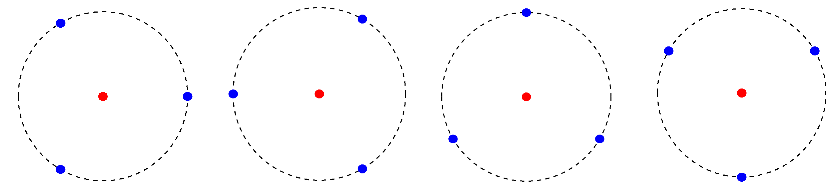
\includegraphics[scale=0.3]{../figures/2Dsketch.png}
		  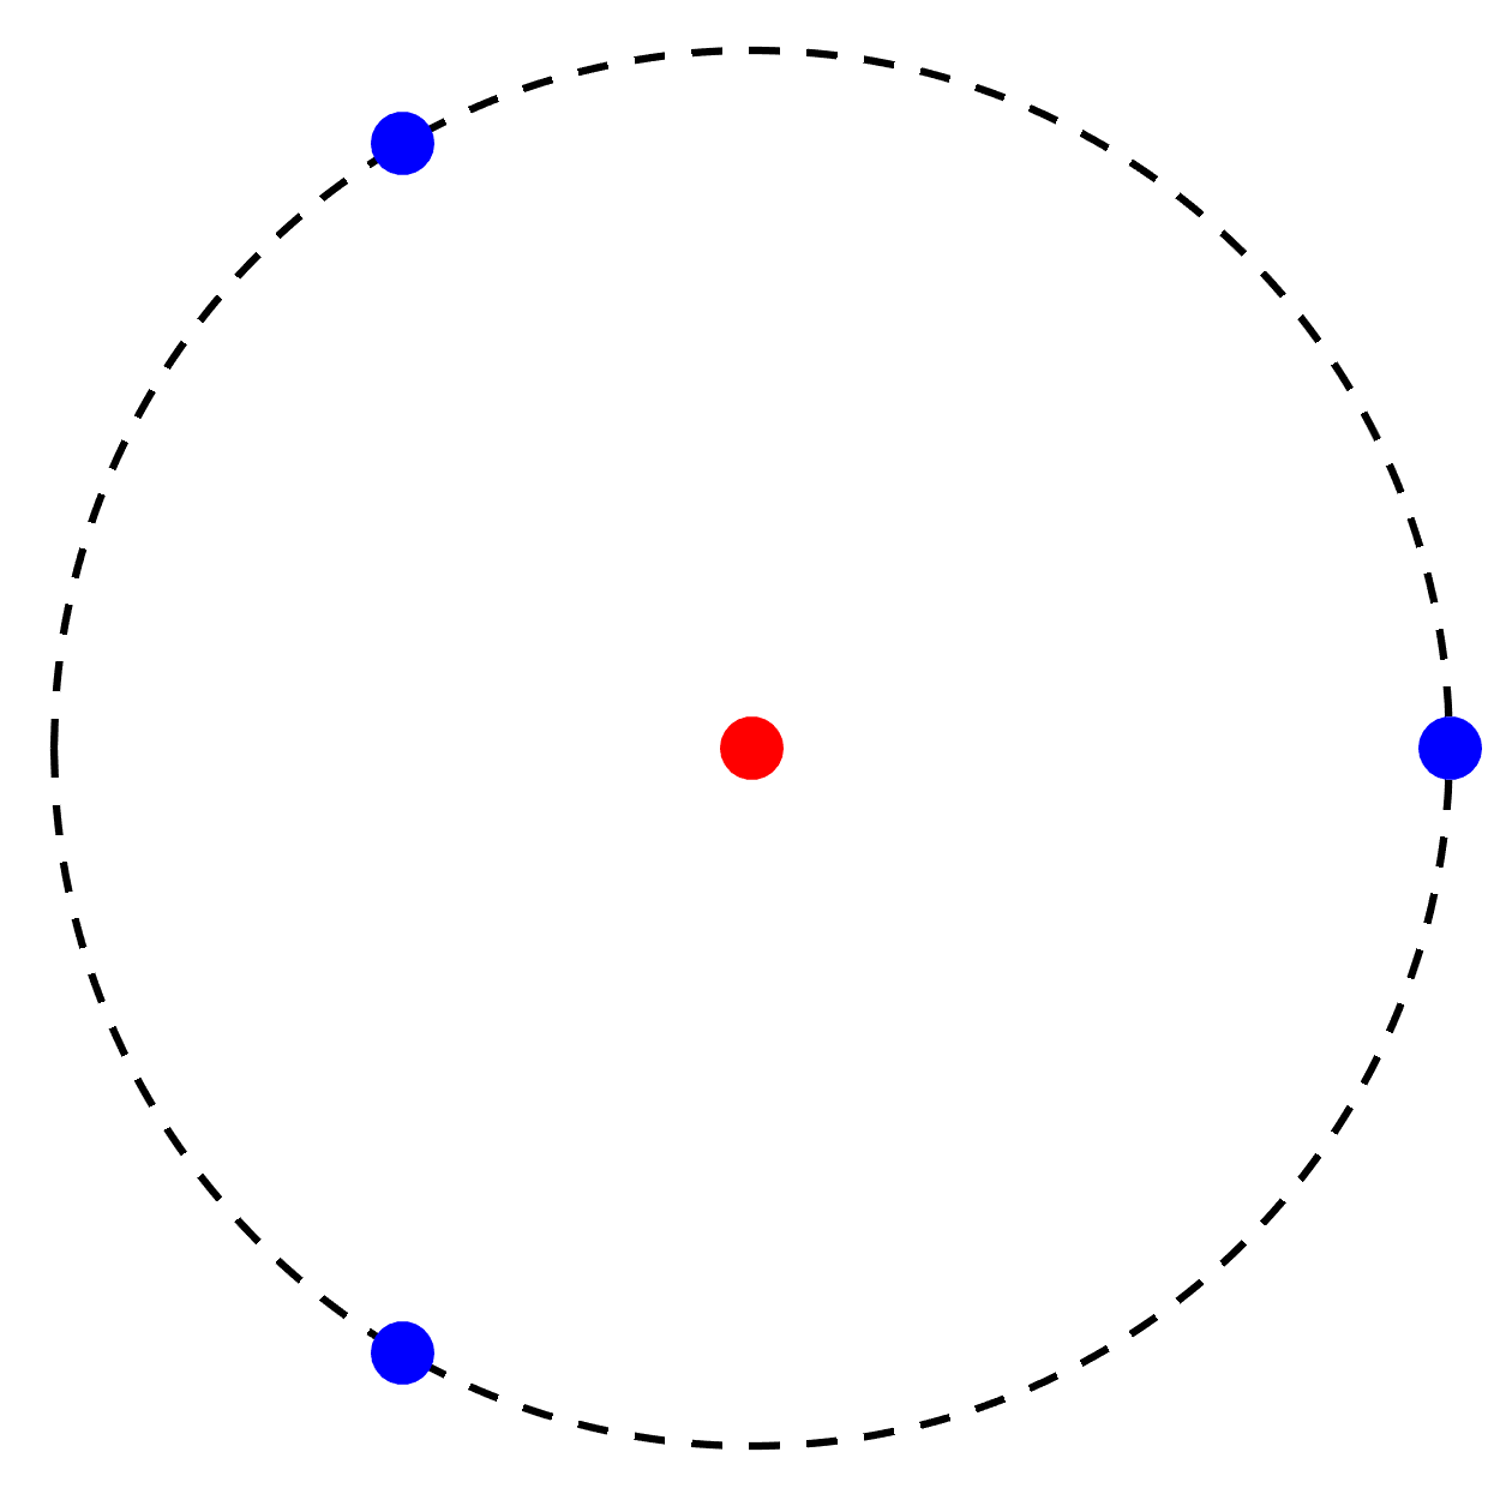
\includegraphics[scale=0.08]{../figures/2D1.png}
		  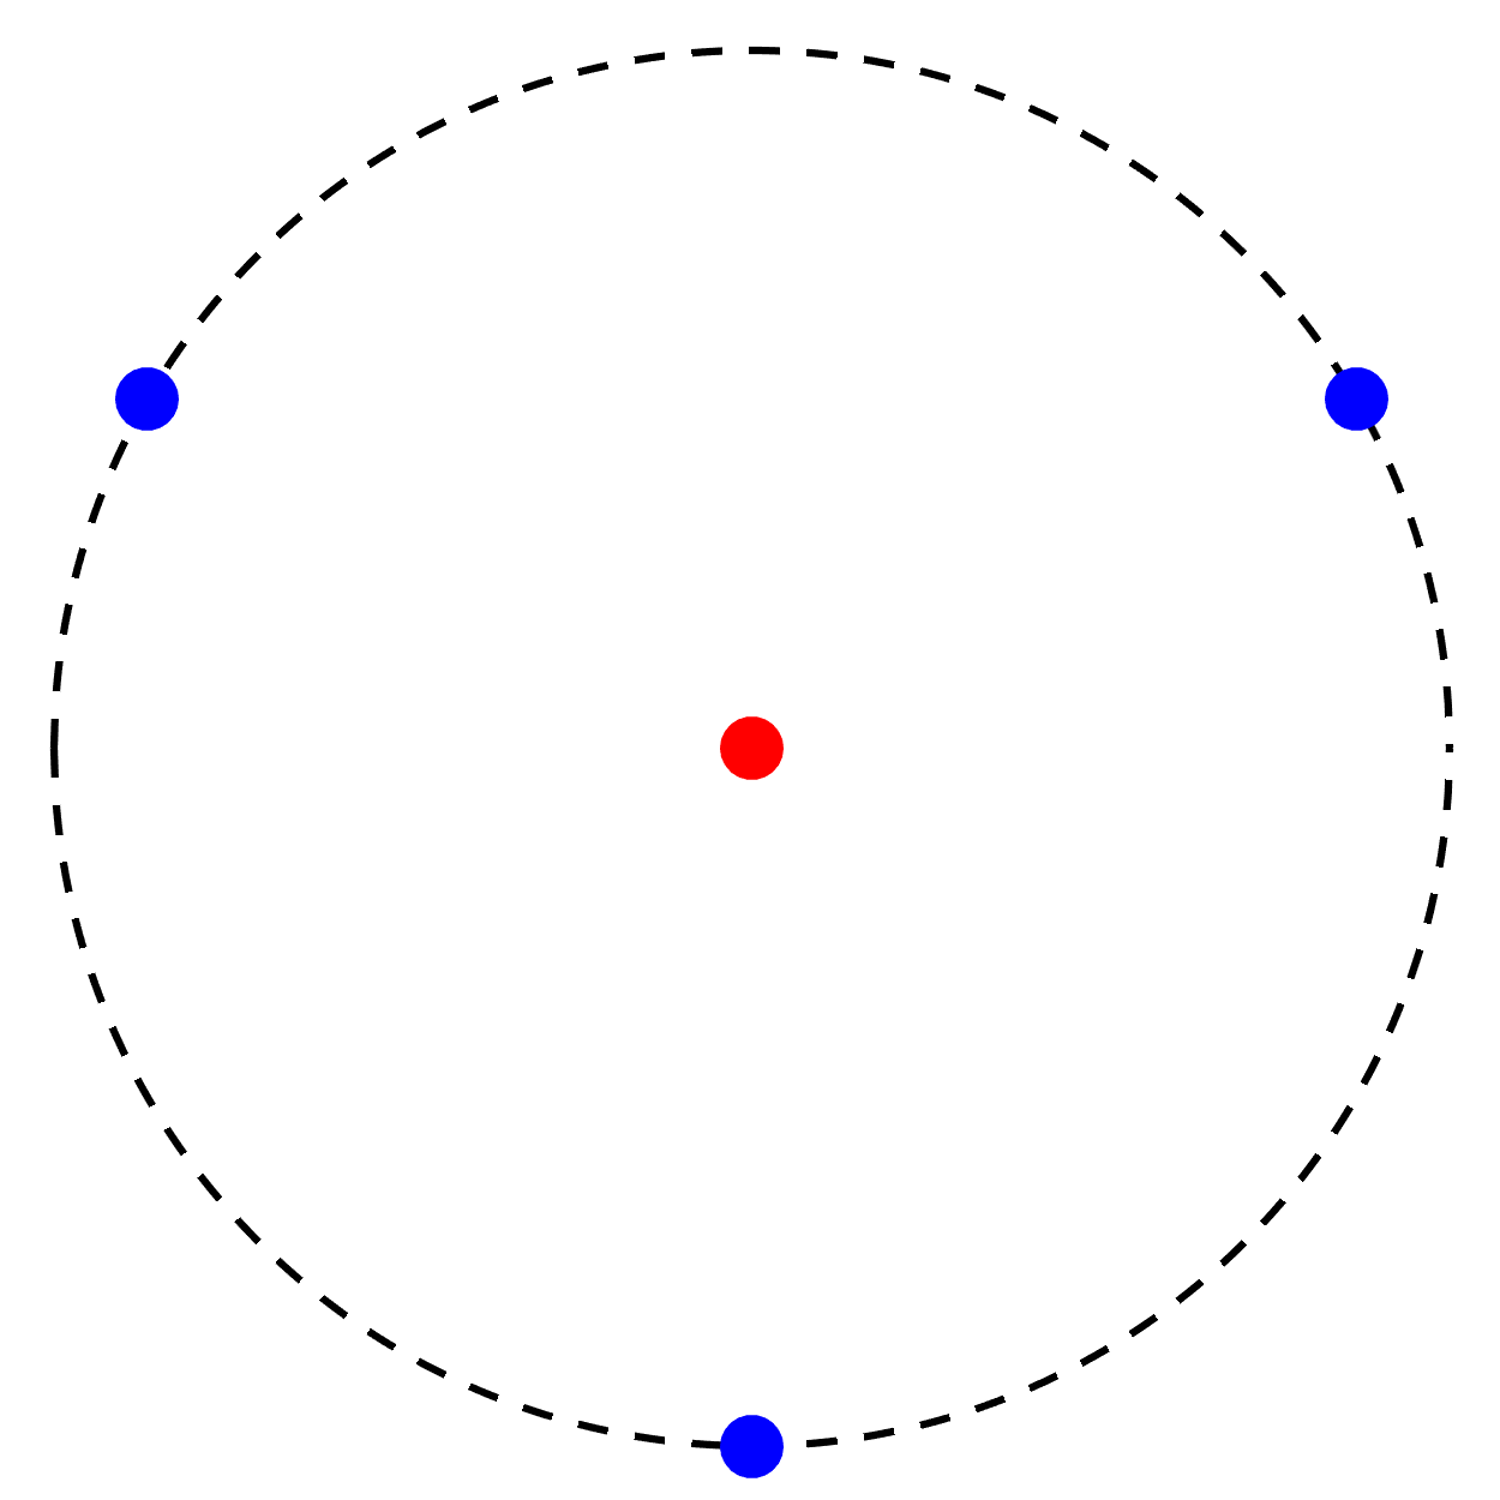
\includegraphics[scale=0.08]{../figures/2D2.png}
		  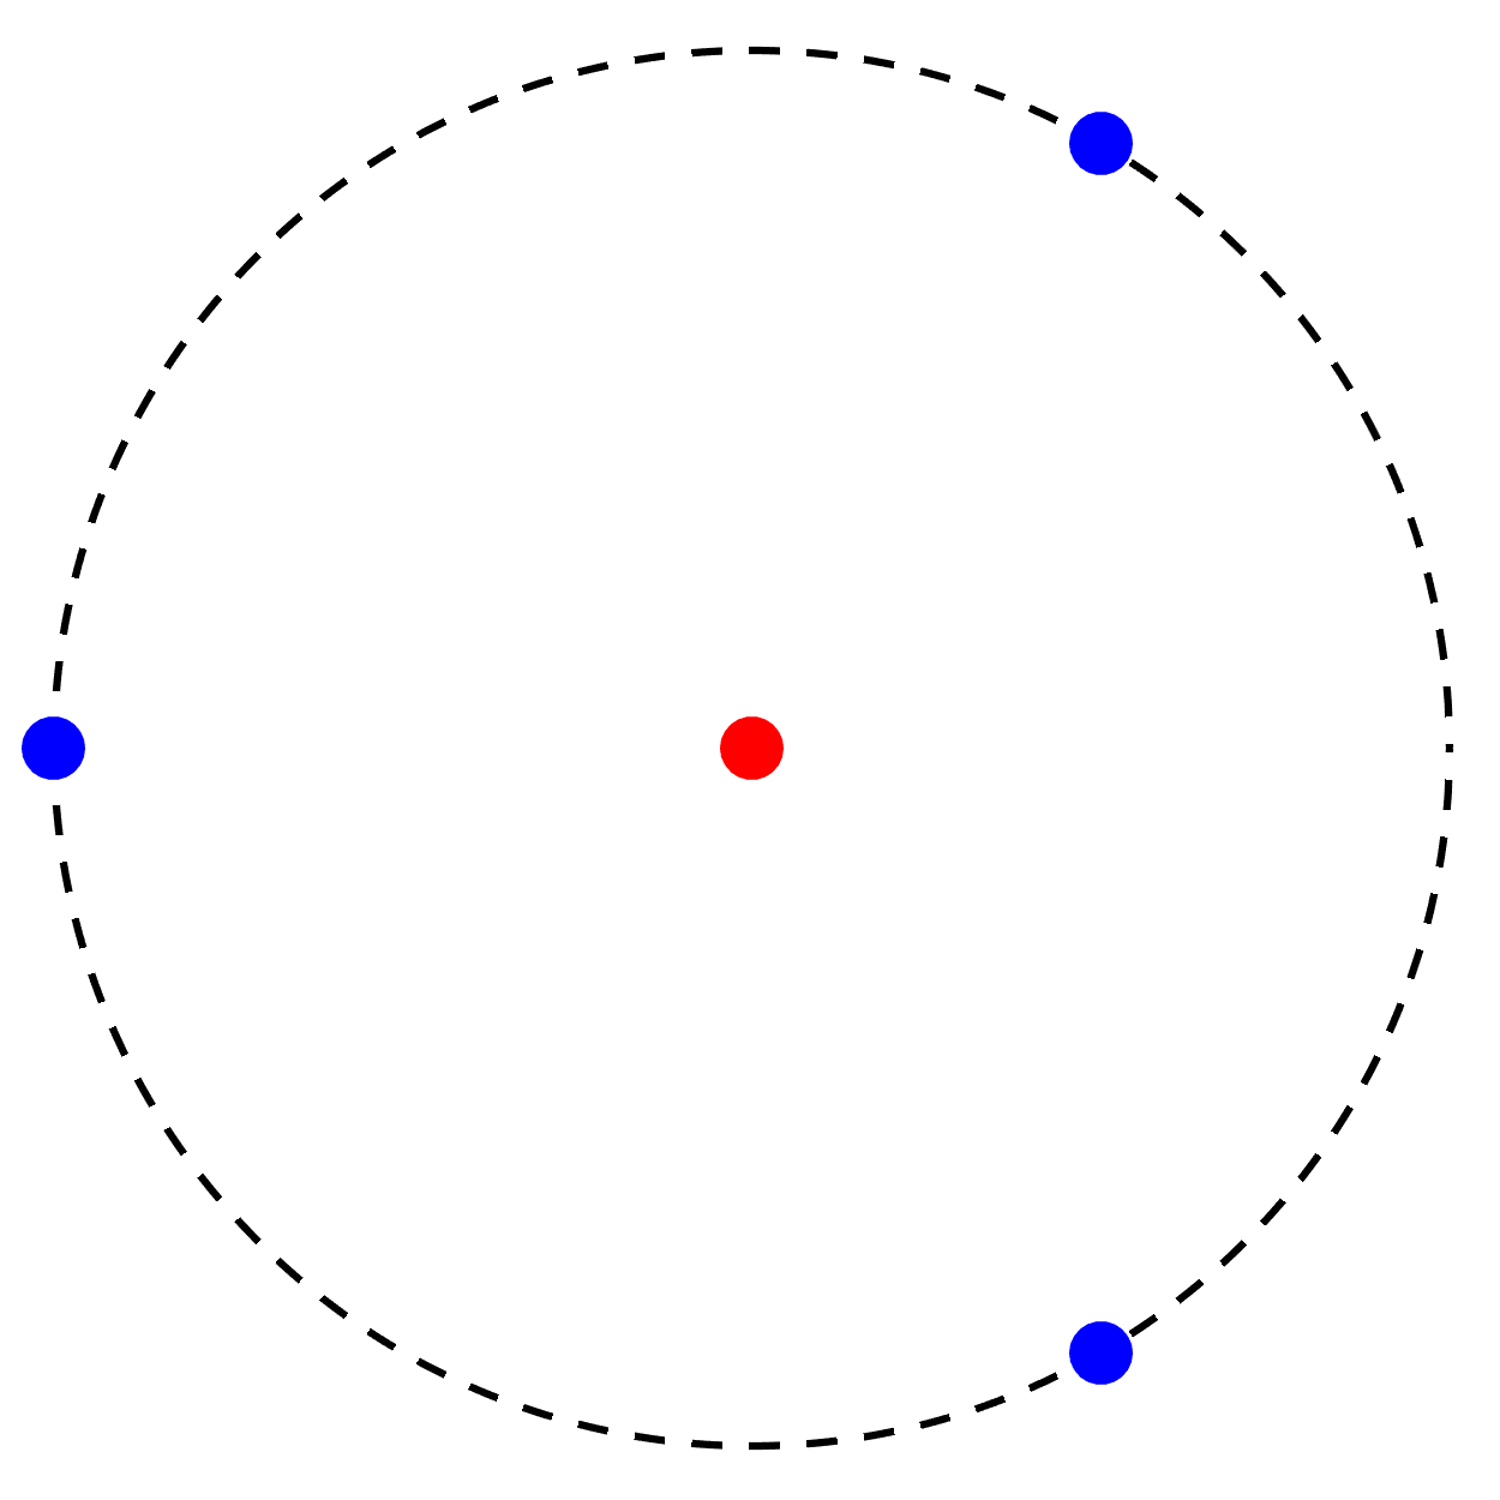
\includegraphics[scale=0.08]{../figures/2D3.png}
		  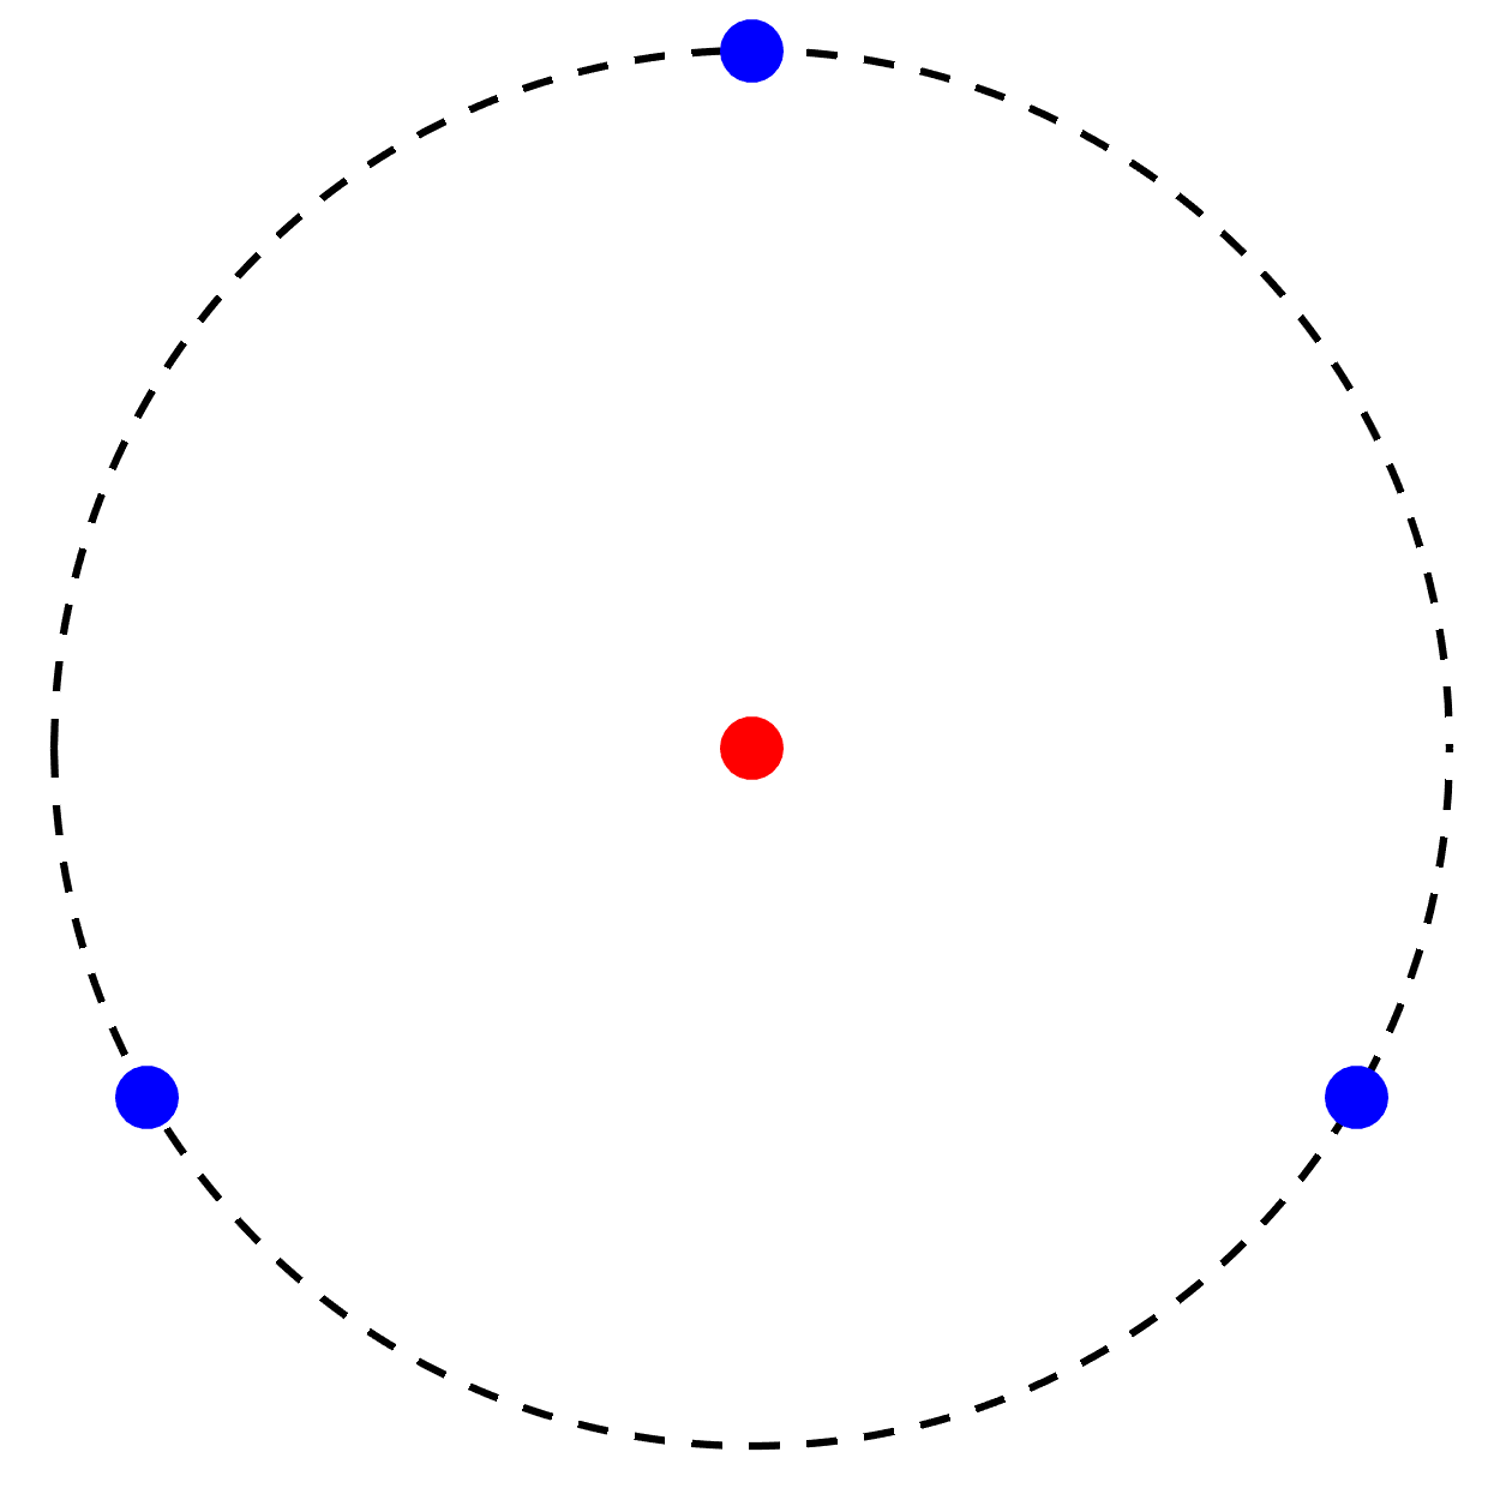
\includegraphics[scale=0.08]{../figures/2D4.png}
	  }
	\subfigure[3D regular simplexes]{
	  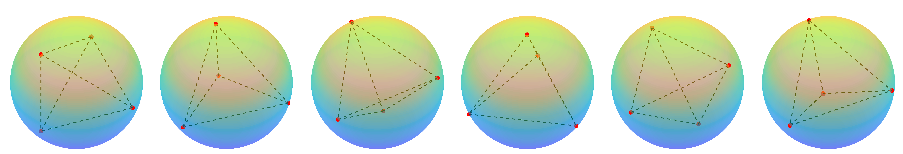
\includegraphics[scale=0.4]{../figures/3Dsketch.png}
	  }
	\caption{The first regular simplexes of sampling the search set $O(x, \rho)$.}
\label{fig:obset:sketch}
\end{figure}
When without a priori knowledge of objective function, the
uniform distribution of these regular simplexes is another
principle to be obeyed.
%%%% How to rotate
Standard schematic simplexes of 2D and
3D cases are given in Fig.\,\ref{fig:obset:sketch}.
It should be noted that there are also other strategies to
discretize $O(x_k,\rho)$. 
For example, the new adding discretized points 
depend on the known information of objective functions. 

To save computational amount, we choose a dynamic refinement
strategy to discretize the search surface and compare function
values in practice. 
%The additional sampling points are generated by rotating the simplex. 
%Consider the uniformly distributed principle, 
%the rotation angle of the new regular simplex is the half of
%angle between the nearest edges. 
Based on the dynamic refinement strategy, we propose the
practical HiCS, see Algorithm \ref{alg:refined}. The computational amount is not
larger than $m_{\max}(d+1)$ in each iteration which is linearly
dependent on the dimension of optimization problems,
$m_{\max}$ is the maximum number of rotation.
Whence, it allows us to treat high-dimensional optimization problems.

\begin{algorithm}[H]
	\caption{Practical HiCS}
	\label{alg:refined}
\begin{algorithmic}[1]
	\STATE Input $x_0$, $\rho$, and $m_{\max}$
	\FOR {$k=0,1,2,\cdots$}
		\STATE Set $m=0$
		\IF {$m\leq m_{\max}$}
			\STATE Discretize $O(x_k,\rho)$ to obtain $O^m_h(x_k,\rho)$
			\IF {$\exists x_j \in O^m_h(x_k,\rho)$, s.t.  $f(x_j)<f(x_k)$}
				\STATE Set $x_{k+1}=x_j$, and $m=m_{\max}+1$
			\ELSE
				\STATE Set $m = m+1$
			\ENDIF
		\ELSE
			\STATE Declare that find a SMP, end program
		\ENDIF
	\ENDFOR
\end{algorithmic}
\end{algorithm}

%\begin{algorithm}[]
%    \caption{Computable HiCS algorithm} 
%    \label{alg:refined}
%\begin{algorithmic}[]
%    \STATE Give $m_{\rm max}$ (the maximum rotation number of
%    regular simplex)
%    \STATE For $k$ iteration in Algorithm\,\ref{alg:HiCS}:
%    \STATE ~~\textbf{Step 1}. Sample the surface
%    $O(x_k, \rho_k)$ with a regular simplex. \\
%    \STATE ~~\textbf{Step 2}. Compare the function values of the
%    samples with $f(x_k)$.
%    \\
%    \hspace{1.5cm} If there exists $\bar{x}$ such that
%    $f(\bar{x})<f(x_k)$, goto \textbf{Step 4}.
%    \\
%    \hspace{1.5cm} Otherwise, goto \textbf{Step 3}.
%    \STATE ~~\textbf{Step 3}. Rotate the regular simplex. If the
%    rotation number is smaller than $m_{\rm max}$, goto
%    \textbf{Step 2}, otherwise, stop iteration.	
%    \STATE ~~\textbf{Step 4}. Declare that the iteration is
%    successful, and set $x_{k+1}= \bar{x}$.
%\end{algorithmic}
%\end{algorithm}

It is evident that once the HiCS converges,
the search space is shrunk to a ball with the radius $\rho$, and
more significantly, the convergent ball contains a SMP.
We will demonstrate this by several numerical experiments in
Sec.\,\ref{sec:experiment}.
It is also noted that the convergent result provides a
good initial value for other optimization approaches, including 
directional search and model-based algorithms.

We can also adjust the search radius $\rho$ in HiCS method 
to improve the approximation precision as done in our previous
work\,\cite{huang2017hill}. Algorithm\,\ref{alg:AHiCS} gives the
process by adaptively changing $\rho$ when Algorithm\,\ref{alg:refined} fails
to find $f(\bar{x})<f(x_k)$, $\bar{x}\in O(x_k, \rho)$ for a fixed $\rho$.
The approximation distance between convergent point and a SMP is
improved when Algorithm\,\ref{alg:AHiCS} converges when $\eta <1$.
Certainly, the search surface can be expanded by setting
control factor $\eta>1$ if required. 
In fact, the Algorithm\,\ref{alg:AHiCS} can be restarted by
fixed $k$ iterations or by other criterions
with different search radius.

%further exploit the potential of
%HiCS algorithm to improve the approximation precision by tuning the
%search radius $\rho$. Algorithm\,\ref{alg:AHiCS} presents a
%strategy to resize the search radius $\rho$. 
%Significant difference of the version from
%Algorithm\,\ref{alg:refined} is adjusting the search radius
%$\rho$ when Algorithm\,\ref{alg:refined} fails to find
%$f(\bar{x})<f(x_k)$, $\bar{x}\in O(x_k, \rho)$ with
%fixed $\rho$. 
%A natural stop criterion of Algorithm\,\ref{alg:AHiCS} is to
%terminate the run when $\rho$ is smaller than a prescribed
%numerical accuracy.
%Certainly, the search surface can be expanded by setting
%control factor $\eta>1$ if required. 
%In fact, Algorithm\,\ref{alg:AHiCS} provides a restart technique by
%fixed the $k$-iterate with different search radius $\rho$.
%
%
\begin{algorithm}[H]
	\caption{Adaptive HiCS}
	\label{alg:AHiCS}
\begin{algorithmic}[1]
	\STATE Input $x_0$, $\rho$, $m_{\max}$,
	\textcolor{black}{$\varepsilon$ and $\eta>0$}
	\IF { \textcolor{black}{ $\rho>\varepsilon$}}
	\FOR {$k=0,1,2,\cdots$}
		\STATE Set $m=0$
		\IF {$m\leq m_{\max}$}
			\STATE Discretize $O(x_k,\rho)$ to obtain $O^m_h(x_k,\rho)$
			\IF {$\exists x_j \in O^m_h(x_k,\rho)$, s.t.  $f(x_j)<f(x_k)$}
			\STATE Set $x_{k+1}=x_j$, 
				and \textcolor{black}{$m=m_{\max}+1$} 
			\ELSE
				\STATE Set $m = m+1$
			\ENDIF
		\ELSE
			\STATE \textcolor{black}{ Set $\rho=\eta\rho$}
		\ENDIF
		\STATE \textcolor{black}{Set $k=k+1$}
	\ENDFOR
\ENDIF
\end{algorithmic}
\end{algorithm}


%\begin{algorithm}[]
%    \caption{Adaptive Stick Hill-Climbing (AHiCS) Algorithm} 
%    \label{alg:AHiCS}
%\begin{algorithmic}[]
%    \STATE \textbf{Initialization:} Choose $x_0$, $\rho$,
%    and control factor $\eta$.
%    \STATE \textbf{For} $k=0,1,2,\dots$
%    \STATE \hspace{0.5cm} Use Algorithm\,\ref{alg:refined} to find
%    $\bar{{x}}\in O(x_k, \rho)$ such that $f(\bar{x})<f(x_k)$.
%         \\
%         \hspace{0.5cm} If such a point is found, then set
%         $x_{k+1}= \bar{x}$.
%          \\
%           \hspace{0.5cm} Otherwise, change the search radius
%          $\rho = \eta \cdot \rho$.
%\end{algorithmic}
%\end{algorithm}


\section{Numerical results}
\label{sec:experiment}

In this section, we choose two kinds of high dimensional optimization functions,
including the unimodal Gaussian function, multimodal problems,
to demonstrate the performance of our proposed algorithm. 
These objective functions are all differentiable. However, it is
emphasized that the HiCS method can be applied to non-differentiable problems. 
In Algorithm\,\ref{alg:refined}, the discretized points of 
search set in each iteration are $m(n+1)$, $n$ is the dimension
of objective function. If not specified, the maximum number of
rotation $m=32$.

\subsection{The unimodal problem: Gaussian function}
\label{subsec:gauss}

The first objective function is the unimodal Gaussian problem
\begin{align}
	f(x) = -20\exp\left(-\sum_{j=1}^d x_j^2 \right),
	\label{eqn:exp1}
\end{align}
which has one minimum $0$ with $f(0)=-20$.
The objective function is differentiable in $\bbR^d$, however,
it quickly diffuses out towards zero out of the upside-down ``bell''. 

%Here we will illustrate the numerical behavior of HiCS method for
%$2$ dimension Gaussian function.

We first investigate the convergent property of HiCS
method for $10$ dimensional Gaussian function using 
$30$ experiments.
In the set of experiments, the search radius $\rho$ is fixed as
$0.3$, start points are all randomly generated in the space $[-1,
1]^{10}$.  For each experiment, the HiCS method indeed converges and
captures a neighbourhood of the peak
$0$ in finite iterations as Theorem \ref{thm:fsc} predicts.
Fig.\,\ref{fig:exp1:randInit} gives the required iterations for
convergence in the $30$ numerical experiments.
\begin{figure}[!htbp]
	\centering
	  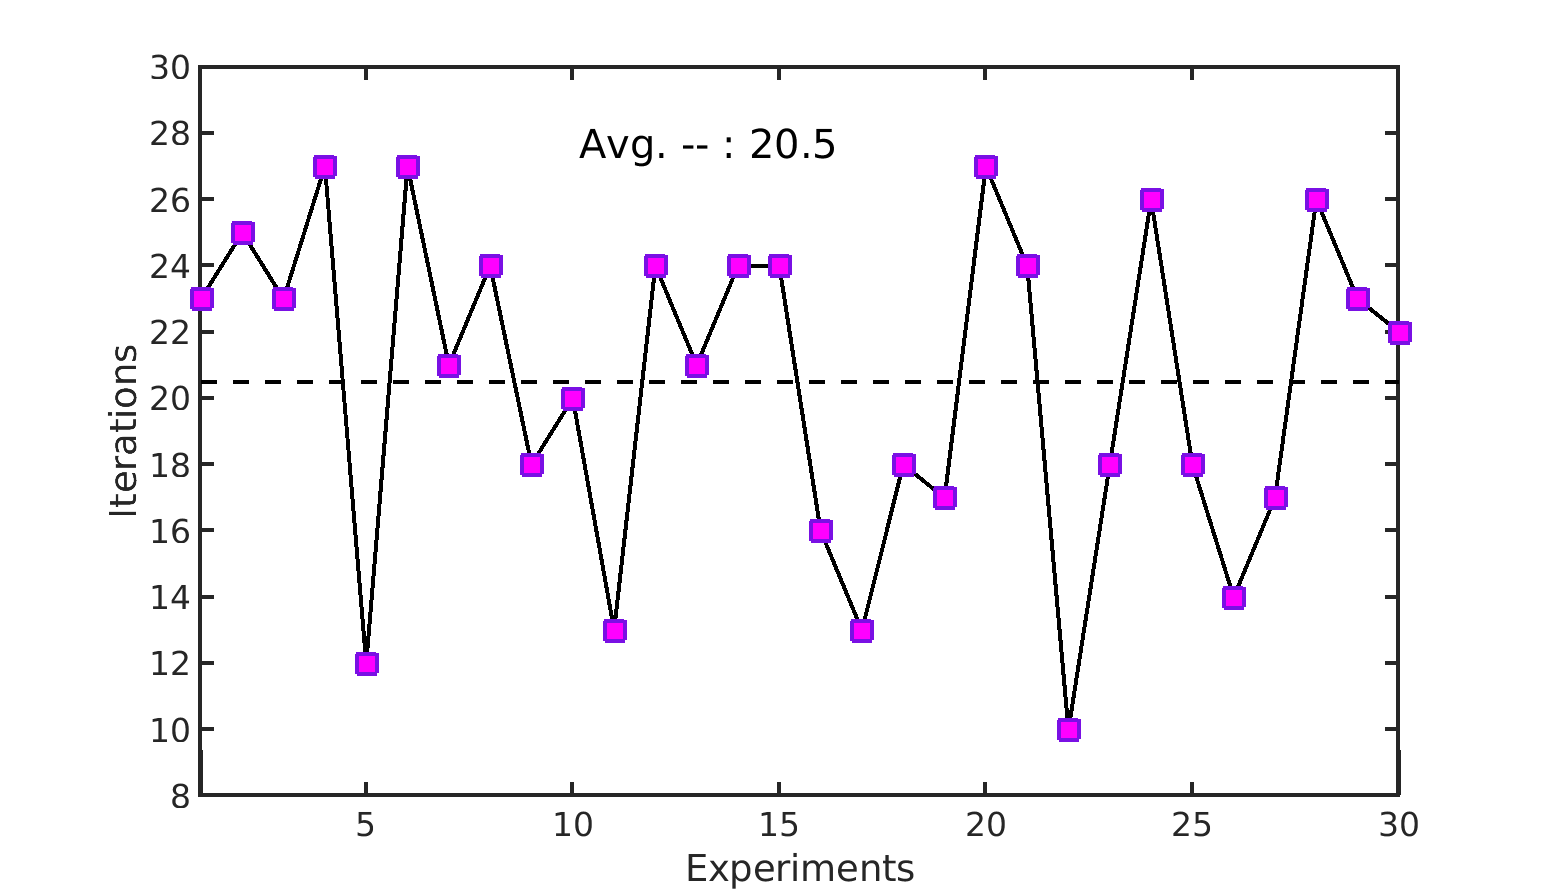
\includegraphics[scale=0.2]{../figures/gauss10Drandr0_3.png}
	  \caption{
	  The required iteration steps of the 
	  HiCS algorithm for the Gaussian function
	  \eqref{eqn:exp1} in $30$ runs with randomly generated start points
	  in the space $[-1, 1]^{10}$, and $\rho=0.3$. 
	  The flat dashed line shows the average.} 
	  \label{fig:exp1:randInit}
\end{figure}
In these $30$ runs, the average iterations of convergence is
$20.5$, while the maximum is $27$, and the minimum is $9$.

%The function satisfies the assumptions of
%Theorem\,\ref{thm:fsc}, therefore, Algorithm\,\ref{alg:HiCS} will
%be convergent in finite steps theoretically.
%To verify this fact, we use random initial values and carry out
%Algorithm\,\ref{alg:HiCS} within $30$ runs.
%In the set of numerical experiments, 
%the search radius $\rho$ is fixed as $0.3$, start points are
%randomly generated in the space $[-1, 1]^{10}$. For each
%experiment, the HiCS method indeed converges and
%captures a neighbourhood of the peak
%$0$ in finite iterations. Fig.\,\ref{fig:exp1:randInit} gives
%the required iterations for convergence in $30$ numerical experiments.
%\begin{figure}[!htbp]
%    \centering
%      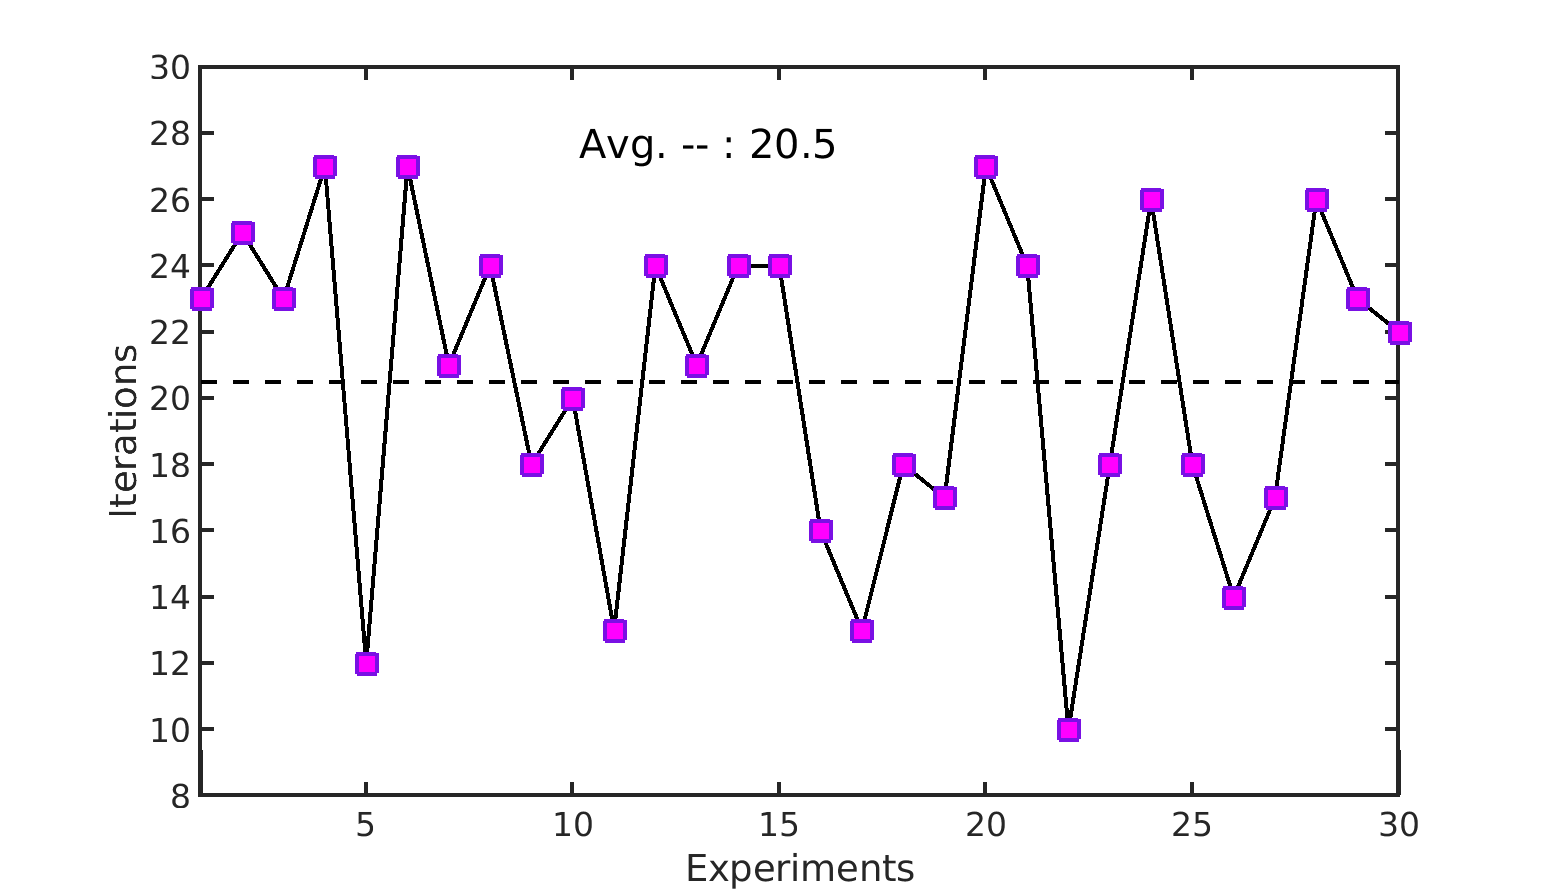
\includegraphics[scale=0.2]{../figures/gauss10Drandr0_3.png}
%      \caption{The iterations of convergence of the 
%      HiCS algorithm to the Gaussian function
%      \eqref{eqn:exp1} in $30$ runs. Start points are randomly
%      generated in the space $[-1, 1]^{10}$, and $\rho=0.3$. 
%      The flat dashed line shows the average.} 
%      \label{fig:exp1:randInit}
%\end{figure}
%In these $30$ runs, the average iterations of convergence is
%$20.5$, while the maximum is $27$, and the minimum is $9$.

Then we decrease the search radius $\rho$ to $0.1$ to observe the
behavior of the HiCS method in $30$ numerical tests. 
The initial values are also randomly generated in the same region.  
The required iterations for convergence is given in
Fig.\,\ref{fig:exp1:randInitr0_1}.
In these $30$ runs, the average iterations of convergence is
$77.2$, while the maximum is $121$, and the minimum is $54$.
From these results, the HiCS approach all converges in
finite iterations. Meanwhile, it is obvious that the value of
$\rho$ affects the number of iterations. 
\begin{figure}[!htbp]
	\centering
	  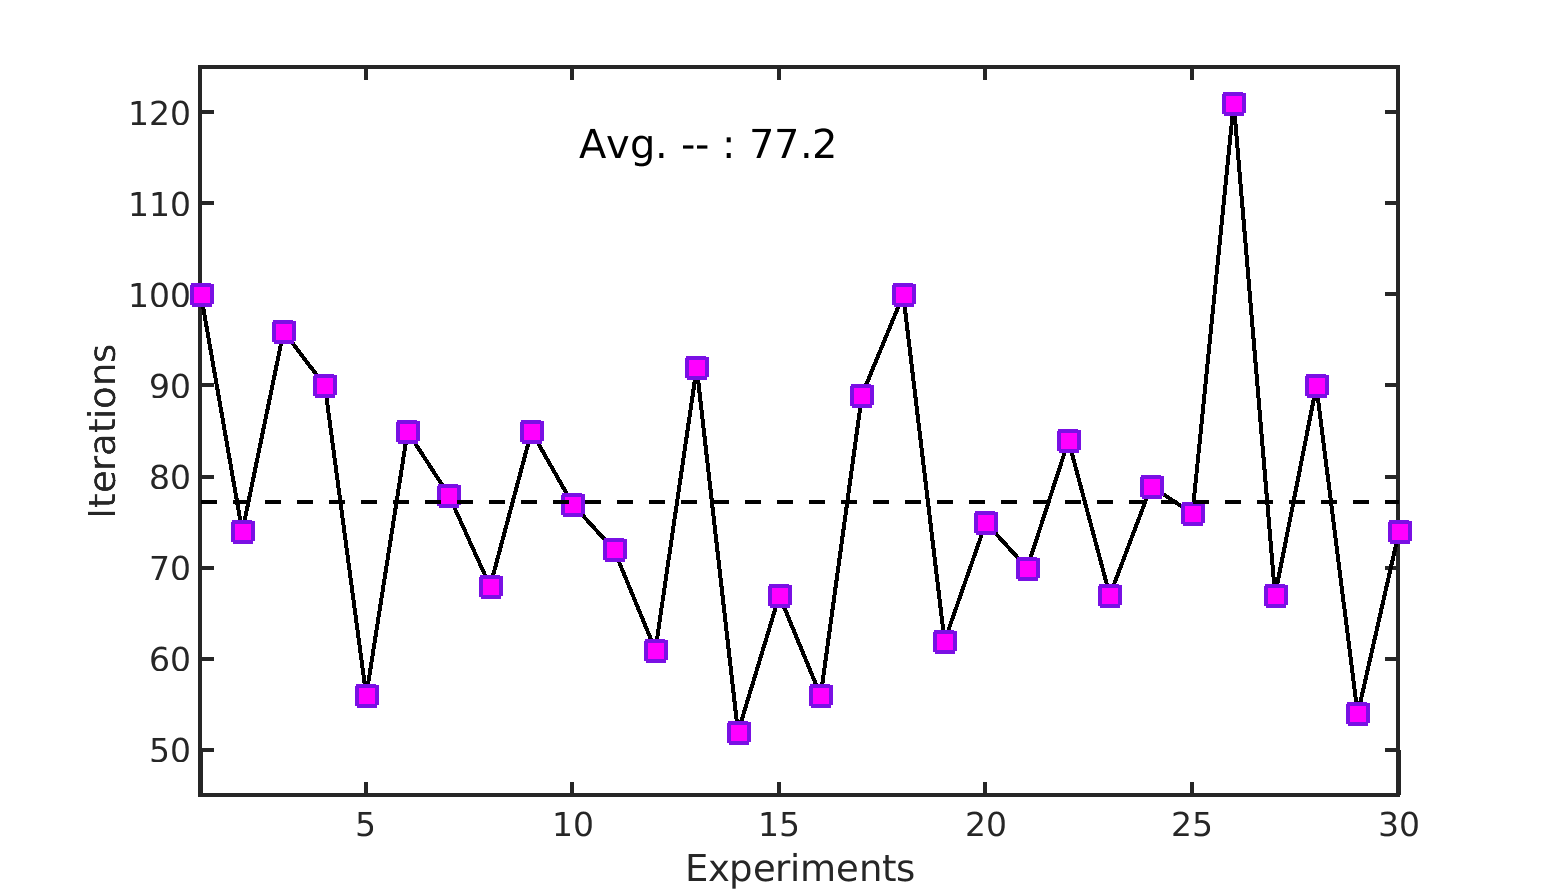
\includegraphics[scale=0.2]{../figures/gauss10Drandr0_1.png}
	  \caption{
	  The required iteration steps of the 
	  HiCS algorithm for the Gaussian function
	  \eqref{eqn:exp1} in $30$ runs with randomly generated start points
	  in the space $[-1, 1]^{10}$, and $\rho=0.1$. 
	  The flat dashed line shows the average.} 
	  \label{fig:exp1:randInitr0_1}
\end{figure}


%The number of iterations is inversely proportional to the
%distance of the initial point and the minimizer.
%When the initial values are far away from the optimal point, the
%algorithm needs more iterations. In contrast, when the initial
%points are close to the minimizer, the method requires less iterations. 
%We also note that when the start point is far away from the peak,
%the derivative-based methods, such as steepest descent method,
%conjugate gradient method and Newton method, would fail since the
%gradient value is almost zero. 
%However, the HiCS algorithm can always approximate the
%peak point. The initial values may yield a few more iterations
%but NOT affect the finite-step convergence as the
%Theorem\,\ref{thm:fsc} shows.

In the following, we apply the adaptive HiCS algorithm to $1000$ dimensional
Gaussian function. The initial value is randomly generated in
domain $[-1000,1000]^{1000}$, the initial search radius $\rho_0 = 2.0$,
and control factor $\eta=(\sqrt{5}-1)/2$. 
Fig.\,\ref{fig:gauss:1000D} presents the iteration process.
The left image in Fig.\,\ref{fig:gauss:1000D} gives
the difference between $f(x_k)$ and $f(0)=-20$. 
The right one in Fig.\,\ref{fig:gauss:1000D} 
plots the changes of search radius $\rho$ and $\ell^2$-distance between
the iterator and the global minimizer $x^*=0$, where $\|x\|_{\ell^2}=\left(
(\sum_{i=1}^d x_i^2) / d\right)^{1/2}$.
From these results, it can be found that the HiCS is convergent
for each $\rho$. Based on the iteration, the adaptive HiCS method
can approximate the global minimum by decreasing the search radius $\rho$. 
Meanwhile, during the iteration, the global minimizer is always in the
search neighbourhood. 
\begin{figure}[!htbp]
	\begin{minipage}[b]{0.5\linewidth}
	\centering{
	  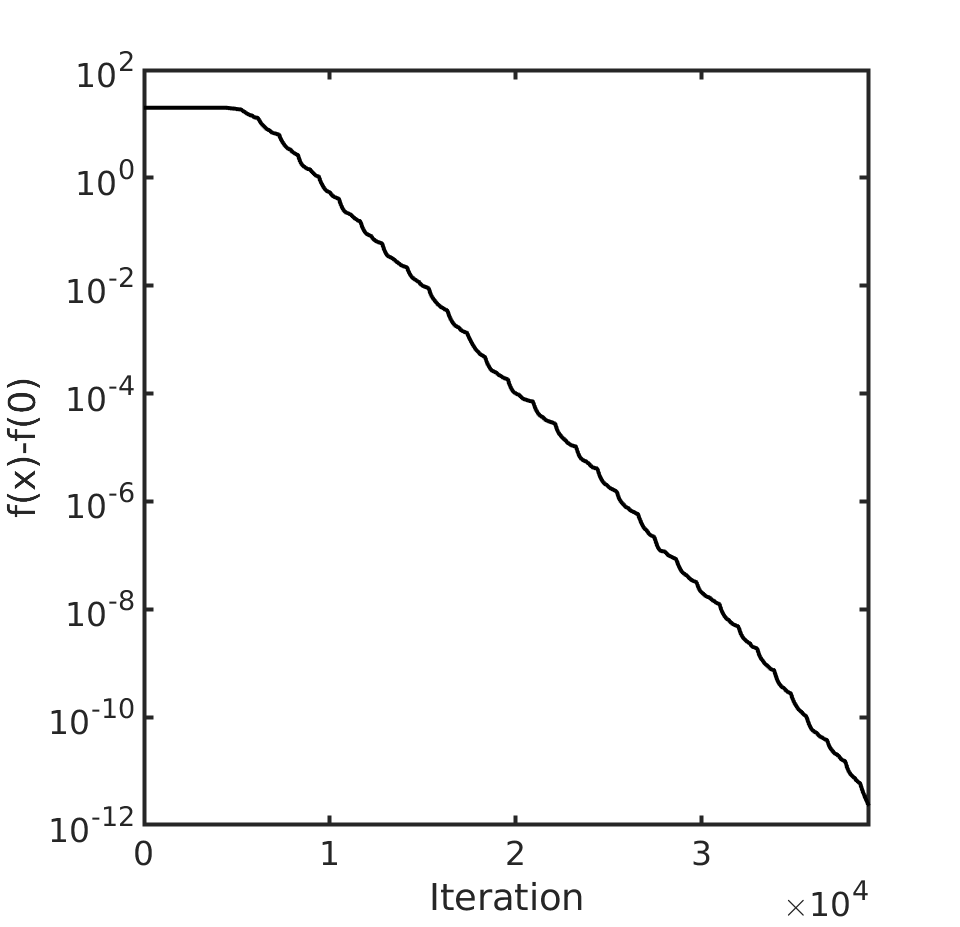
\includegraphics[scale=0.25]{../figures/gauss1000D.png}
	  }
%    \centerline{(a) }
	\end{minipage}
	\begin{minipage}[b]{0.5\linewidth}
	\centering{
	  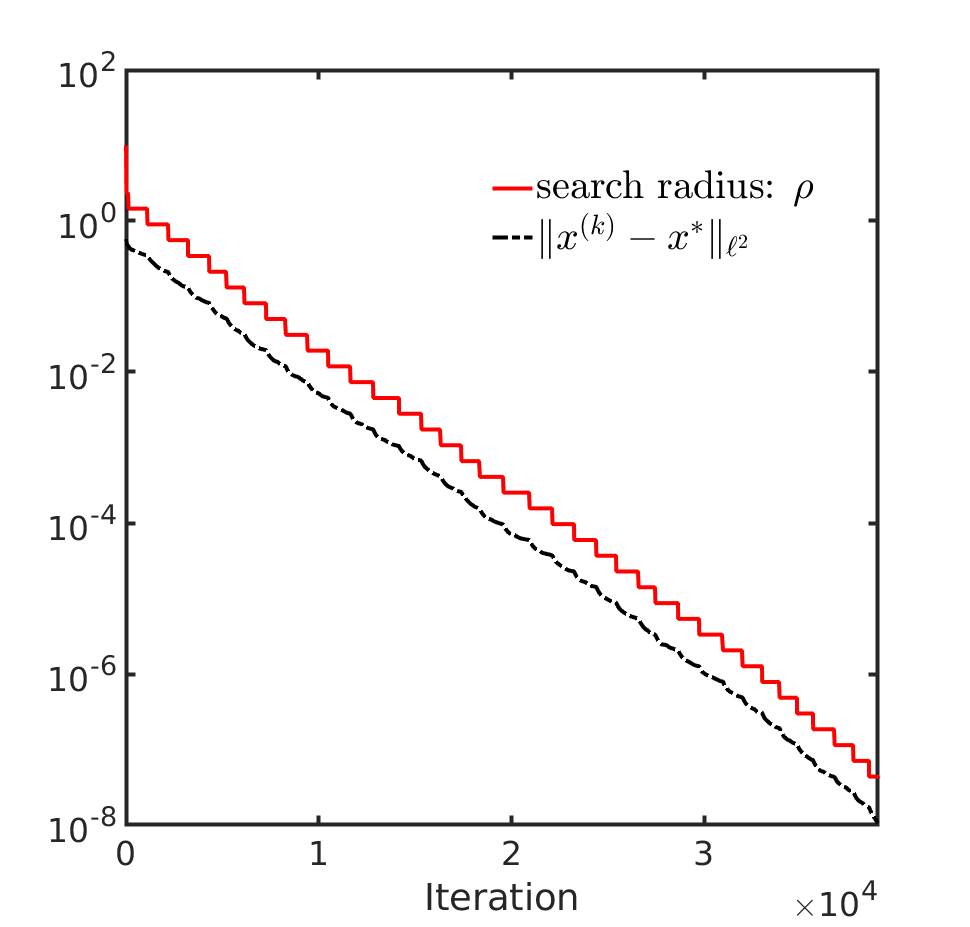
\includegraphics[scale=0.25]{../figures/gauss1000D_dist.png}
	  }
%    \centerline{(b) }
	\end{minipage}
	  \caption{The iteration process of the adaptive HiCS method to 1000
	  dimensional Gaussian function. 
	  Start point is randomly generated in the space $[-1000,
	  1000]^{1000}$, $\rho=2.0$ and control factor
	  $\eta=(\sqrt{5}-1)/2$. The left plot is the energy
	  difference, and the right one is the search radius and 
	  the $\ell^2$ distance between the current iterator and the
	  global minimizer $x^*=0$.
	  } 
	  \label{fig:gauss:1000D}
\end{figure}

%Then we take an example to further observe the numerical behavior
%of the HiCS algorithm.
%Tab.\,\ref{tab:gauss:CHC} shows the iterative procedure of the
%HiCS approach in detail when the start point is
%$x_0=(6.7, -8.0)$ with fixed search radius $\rho=1.0$. 
%In the Tab.\,\ref{tab:gauss:CHC}, the first and second columns show
%the number of iterations and rotation simplexes when applying
%HiCS
%method. The third column gives the $\ell^2$-distance between
%iterator and the global minimizer $0$, where
%$\|x\|_{\ell^2}=\left(\sum_{i=1}^n x_i^2 \right)^{1/2}$.
%The fourth column is the function value on iterator.
%\begin{table}[!htbp]
%\begin{center}
%\caption{\label{tab:gauss:CHC}The iterative procedure of 
%HiCS algorithm with $\rho=1.0$ when the initial value
%is $x_0=(6.7, -8,0)$.}	
%\begin{tabular}{|c|c|c|c|}
% \hline
%Iteration & $m$ & $\ell^2$-distant &  Function value
% \\\hline
% 1 & 1 & 10.435037135 & -5.1247639412e-47 \\
% \hline
% 2 & 1 &  9.4516450176 & -1.5955605034e-38 \\
% \hline
% 3 & 1 &  8.4721418236 & -6.7230095025e-31 \\
% \hline
% 4 & 1 & 7.4980517882 & -3.8337625366e-24 \\
% \hline
% 5 & 1 &  6.5317971614 & -2.9586781839e-18 \\
% \hline
% 6 & 1 &  5.5774517207 & -3.0901622718e-13 \\
% \hline
% 7 & 1 &  4.6423659094 & -4.3679320991e-09 \\
% \hline
% 8 & 1 &  3.7410098605 & -8.3556743824e-06 \\
% \hline
% 9 & 1 &  2.9049523775 & -2.1632074620e-03 \\
% \hline
% 10 & 1 &  2.2096021938 & -7.5792437378e-02 \\
% \hline
% 11 & 1 &  1.8237147240 & -3.5938885990e-01 \\
% \hline
% 12 & 1 &  1.2175146221 & -2.2710521764e+00 \\
% \hline
% 13 & 1 &  0.96225536865 & -3.9616067919e+00 \\
% \hline
% 14 & 32 & 0.28695270523 & -9.2095707106e+00 \\
% \hline
%\end{tabular}
%\end{center}
%\end{table}
%The results show that the iterates can be updated efficiently to
%capture a neighbourhood of the minimizer $0$ within $14$ steps. 
%The convergent result reduces the search space and
%provides a good start position $(0.3, -0.1)$ to further
%approximate the minimizer to high precision with other
%optimization algorithms.
%Due to the good analytical nature of objective function, the
%derivative-based methods or adaptive HiCS method (see
%Algorithm\,\ref{alg:AHiCS}) are both good choices of finding the
%minimizer with the above convergent results. 

\subsection{The multimodal problems: Ackley and Arwhead functions}
\label{subsec:minmulit}

The second test objective function is the Ackley
function\,\cite{dieterich2012empirical} which is a widely used 
benchmark function for testing optimization algorithms.
The expression of the Ackley function can be written as
\begin{align}
	f(x) =
	-20\cdot\exp\left(-\frac{1}{5}\cdot\sqrt{\frac{1}{d}\sum_{i=1}^d
	x_i^2}\right)-
	\exp\left(\frac{1}{d}\sum_{i=1}^d \cos(2\pi x_i)\right)+20+e,
	\label{eqn:ackley}
\end{align}
where $n$ is the dimension.
Ackley function has many local minima and a unique global
minimum of $0$ with $f(0)=0$, which poses a risk for
optimization algorithms to be trapped into one of local
minima, such as the traditional hill-climbing method\,\cite{back1996evolutionary}.
Our previous result has shown that the HiCS method can capture
different local minimizer and the global minimizer for 2
dimensional problem through the choice of different $\rho$\,\cite{huang2017hill}.
In this subsection, we will apply the improved HiCS
algorithm to higher dimensional Ackley function. 
In the following simulation, the control factor
$\eta=(\sqrt{5}-1)/2$.

\begin{table}[!hbpt]
\caption{
The successful number $N_s$ of capturing the global minimizer for
each different initial search radius $\rho_0$ when applying the
adaptive HiCS method to $100$ dimensional Ackley function from 100
time numerical experiments. 
The initial values are randomly generated in $[-10,10]^{100}$.
}
\label{tab:ackley100D:AHiCS}
\begin{center}
\begin{tabular}{|c|c|c|c|c|c|c|c|c|c|c|}
 \hline
  $\rho_0$  & 2.0 & 1.8 & 1.6 & 1.4 & 1.2 & 1.0 & 0.8 & 0.6 & 0.4 & 0.2 
 \\\hline
  $N_s$     & 98  & 99  & 97  & 73  & 93  & 100 & 99  & 84  & 76 & 57 
\\\hline \hline
 $\rho_0$ & 0.1 & 0.09 & 0.08 & 0.07 & 0.06 & 0.05 & 0.04 & 0.03& 0.02 & 0.01
 \\\hline
  $N_s$& 75 & 79 & 72 & 69 & 84 &86 & 52 & 0 & 0 & 0
\\ \hline
\end{tabular}
\end{center}
\end{table}
We first take $100$ dimensional Ackley function as an example to
test the performance of our proposed algorithm for finding minimizers. 
We run adaptive HiCS method 100 times for each different initial
search radius $\rho_0$ from $0.01$ to $2.0$.
The start points are all randomly generated in $[-10,10]^{100}$.
The convergent criterion is the search radius smaller than $10^{-10}$.
Tab.\,\ref{tab:ackley100D:AHiCS} gives the successful number
$N_s$ of capturing the global minimizer.  
When the algorithm is successful, the distance between the
convergent iterator and the global minimizer is smaller than the
search radius $\rho < 10^{-10}$.
From these results, it is easy to find that our method is able to
approximate the global minimizer. 
The value of $\rho_0$ heavily affects the probability of
obtaining the global minimizer. 
When $\rho_0 > 0.04$, the adaptive HiCS can find the global
minimizer with high probability. 
When $\rho_0$ is about $0.04$, 
the successful probability is falling quickly to about $50\%$. 
As $\rho_0$ decreases to smaller than $0.03$, the HiCS could not
find the global minimizer.
In addition, it should be pointed out that these so-called unsuccessful
experiments have obtained other local minimizers. 



%The first numerical test
%is taking $\rho=2.0$ to observe the iteration process of the HiCS
%approach. The corresponding iteration process 
%is presented in Tab.\,\ref{tab:ackley100D:HiCS}
%for $100$ dimensional Ackley function. HiCS takes $365$ iterations
%to obtain a SMP. In the first $353$ steps, HiCS can efficiently find a better
%position merely using a regular simplex, i.e., within $101$ function evaluations.
%\begin{table}[!htbp]
%\caption{Iteration process of HiCS with constant $\rho_0=2.0$ to
%$100$ dimensional Ackley function.
%}
%\label{tab:ackley100D:HiCS}
%\begin{center}
%\begin{tabular}{|c|c|c|}
% \hline
%    Iter. & $\ell^2$-distance &  Fun. Val.
% \\\hline
% \makecell{ 1 (1-353) } & \makecell{ 43.76984 \\ $\downarrow$ \\
% 5.67057 }
% & \makecell{  13.40276 \\ $\downarrow$ \\ 3.65003 }
% \\\hline
% 3  &\textcolor{blue}{5.76768} & 3.64961
% \\\hline
% 5  & \textcolor{blue}{5.84103} &3.64579
% \\\hline
%  5  & 5.75717 &3.63706
% \\\hline
%1  & 5.72732  & 3.63154
% \\\hline
% 1 &   5.68106  & 3.63021
% \\\hline
% 6 &   5.67458  & 3.60655
% \\\hline
% 12 &  5.76181  &  3.60569
% \\\hline
% 5  & \textcolor{blue}{5.84496}  & 3.59674
% \\\hline
%1  & 5.76528  & 3.59377
% \\\hline
%1  & 5.71754  & 3.59277
% \\\hline
% 2  & \textcolor{blue}{5.90908} &  3.59054
% \\\hline
% 32 ($m_{max}$) & \textcolor{blue}{5.93767} &  3.58252
% \\\hline
%\end{tabular}
%\end{center}
%\end{table}
%After convergence, we can continue to apply the adaptive HiCS method.
%Fig.\,\ref{fig:ackley100D:AHiCS} gives the distance
%between the function value and the global minimum, and the
%$\ell^2$-distance between the current position and the global minimizer. 
%It is easy to find that the iterate indeed approximates the
%global minimizer as the iteration increases.
%\begin{figure}[!htbp]
%    \centering
%      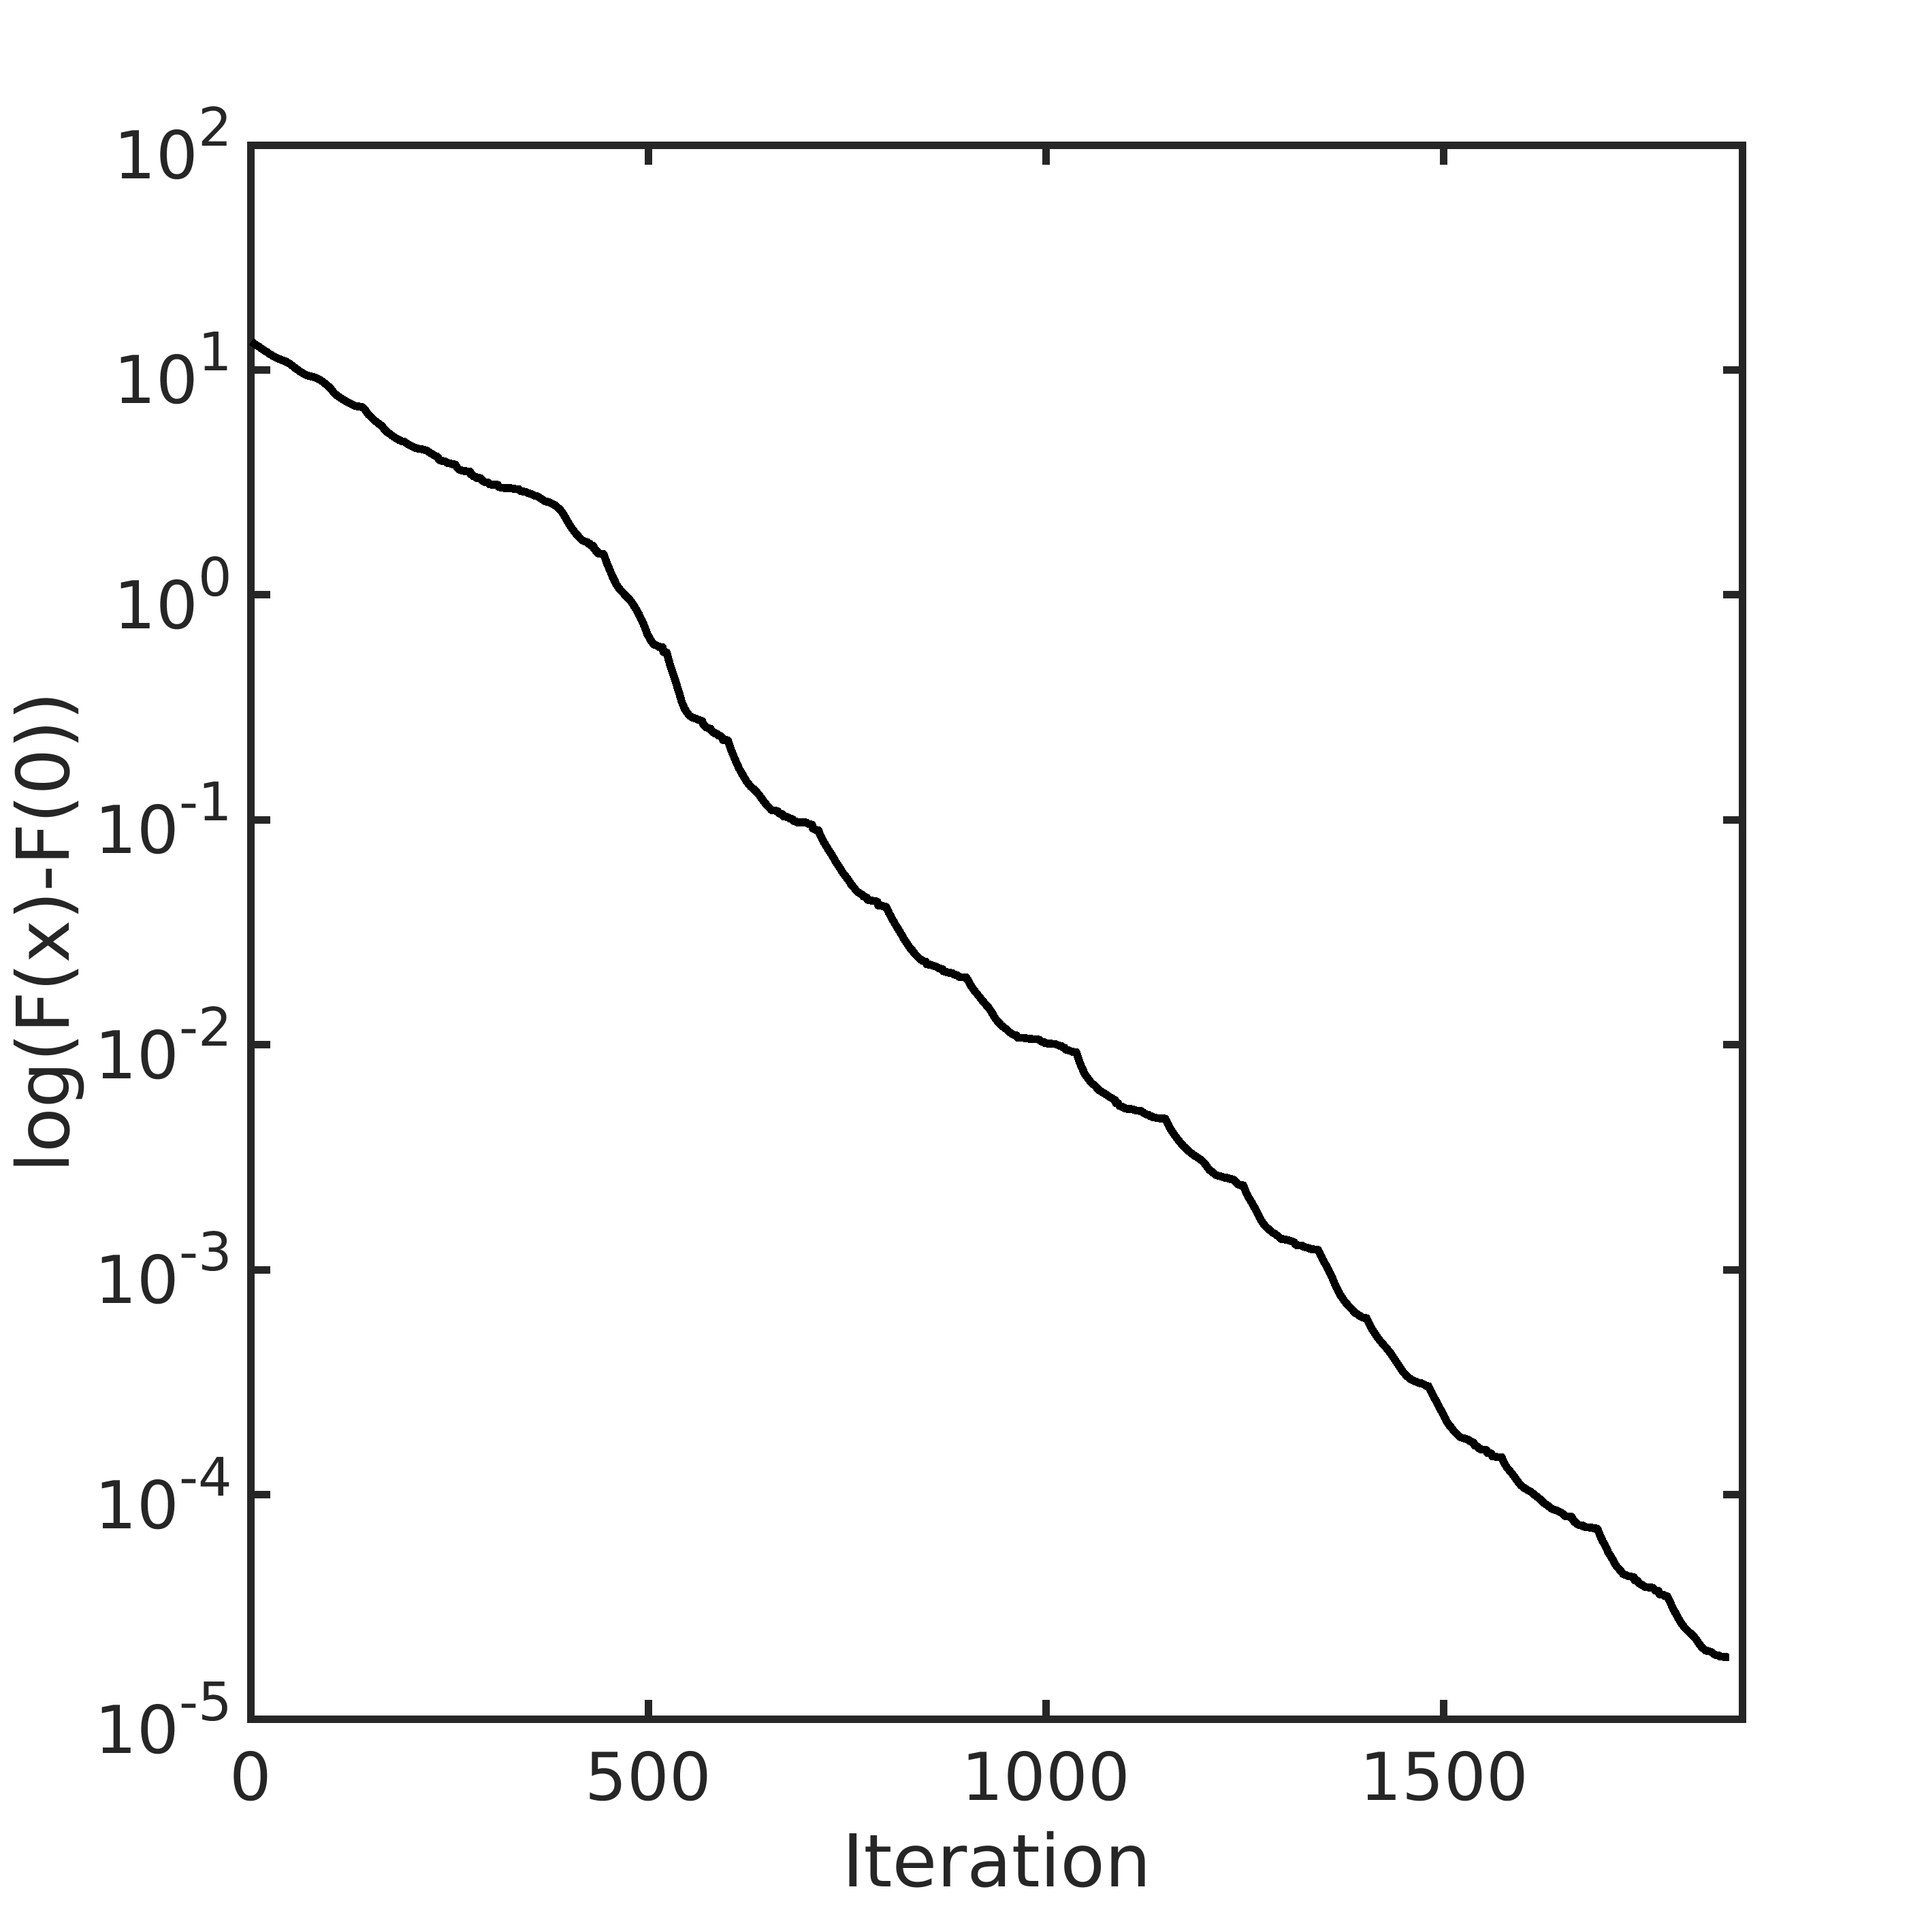
\includegraphics[scale=0.25]{../figures/ackley100D.png}
%      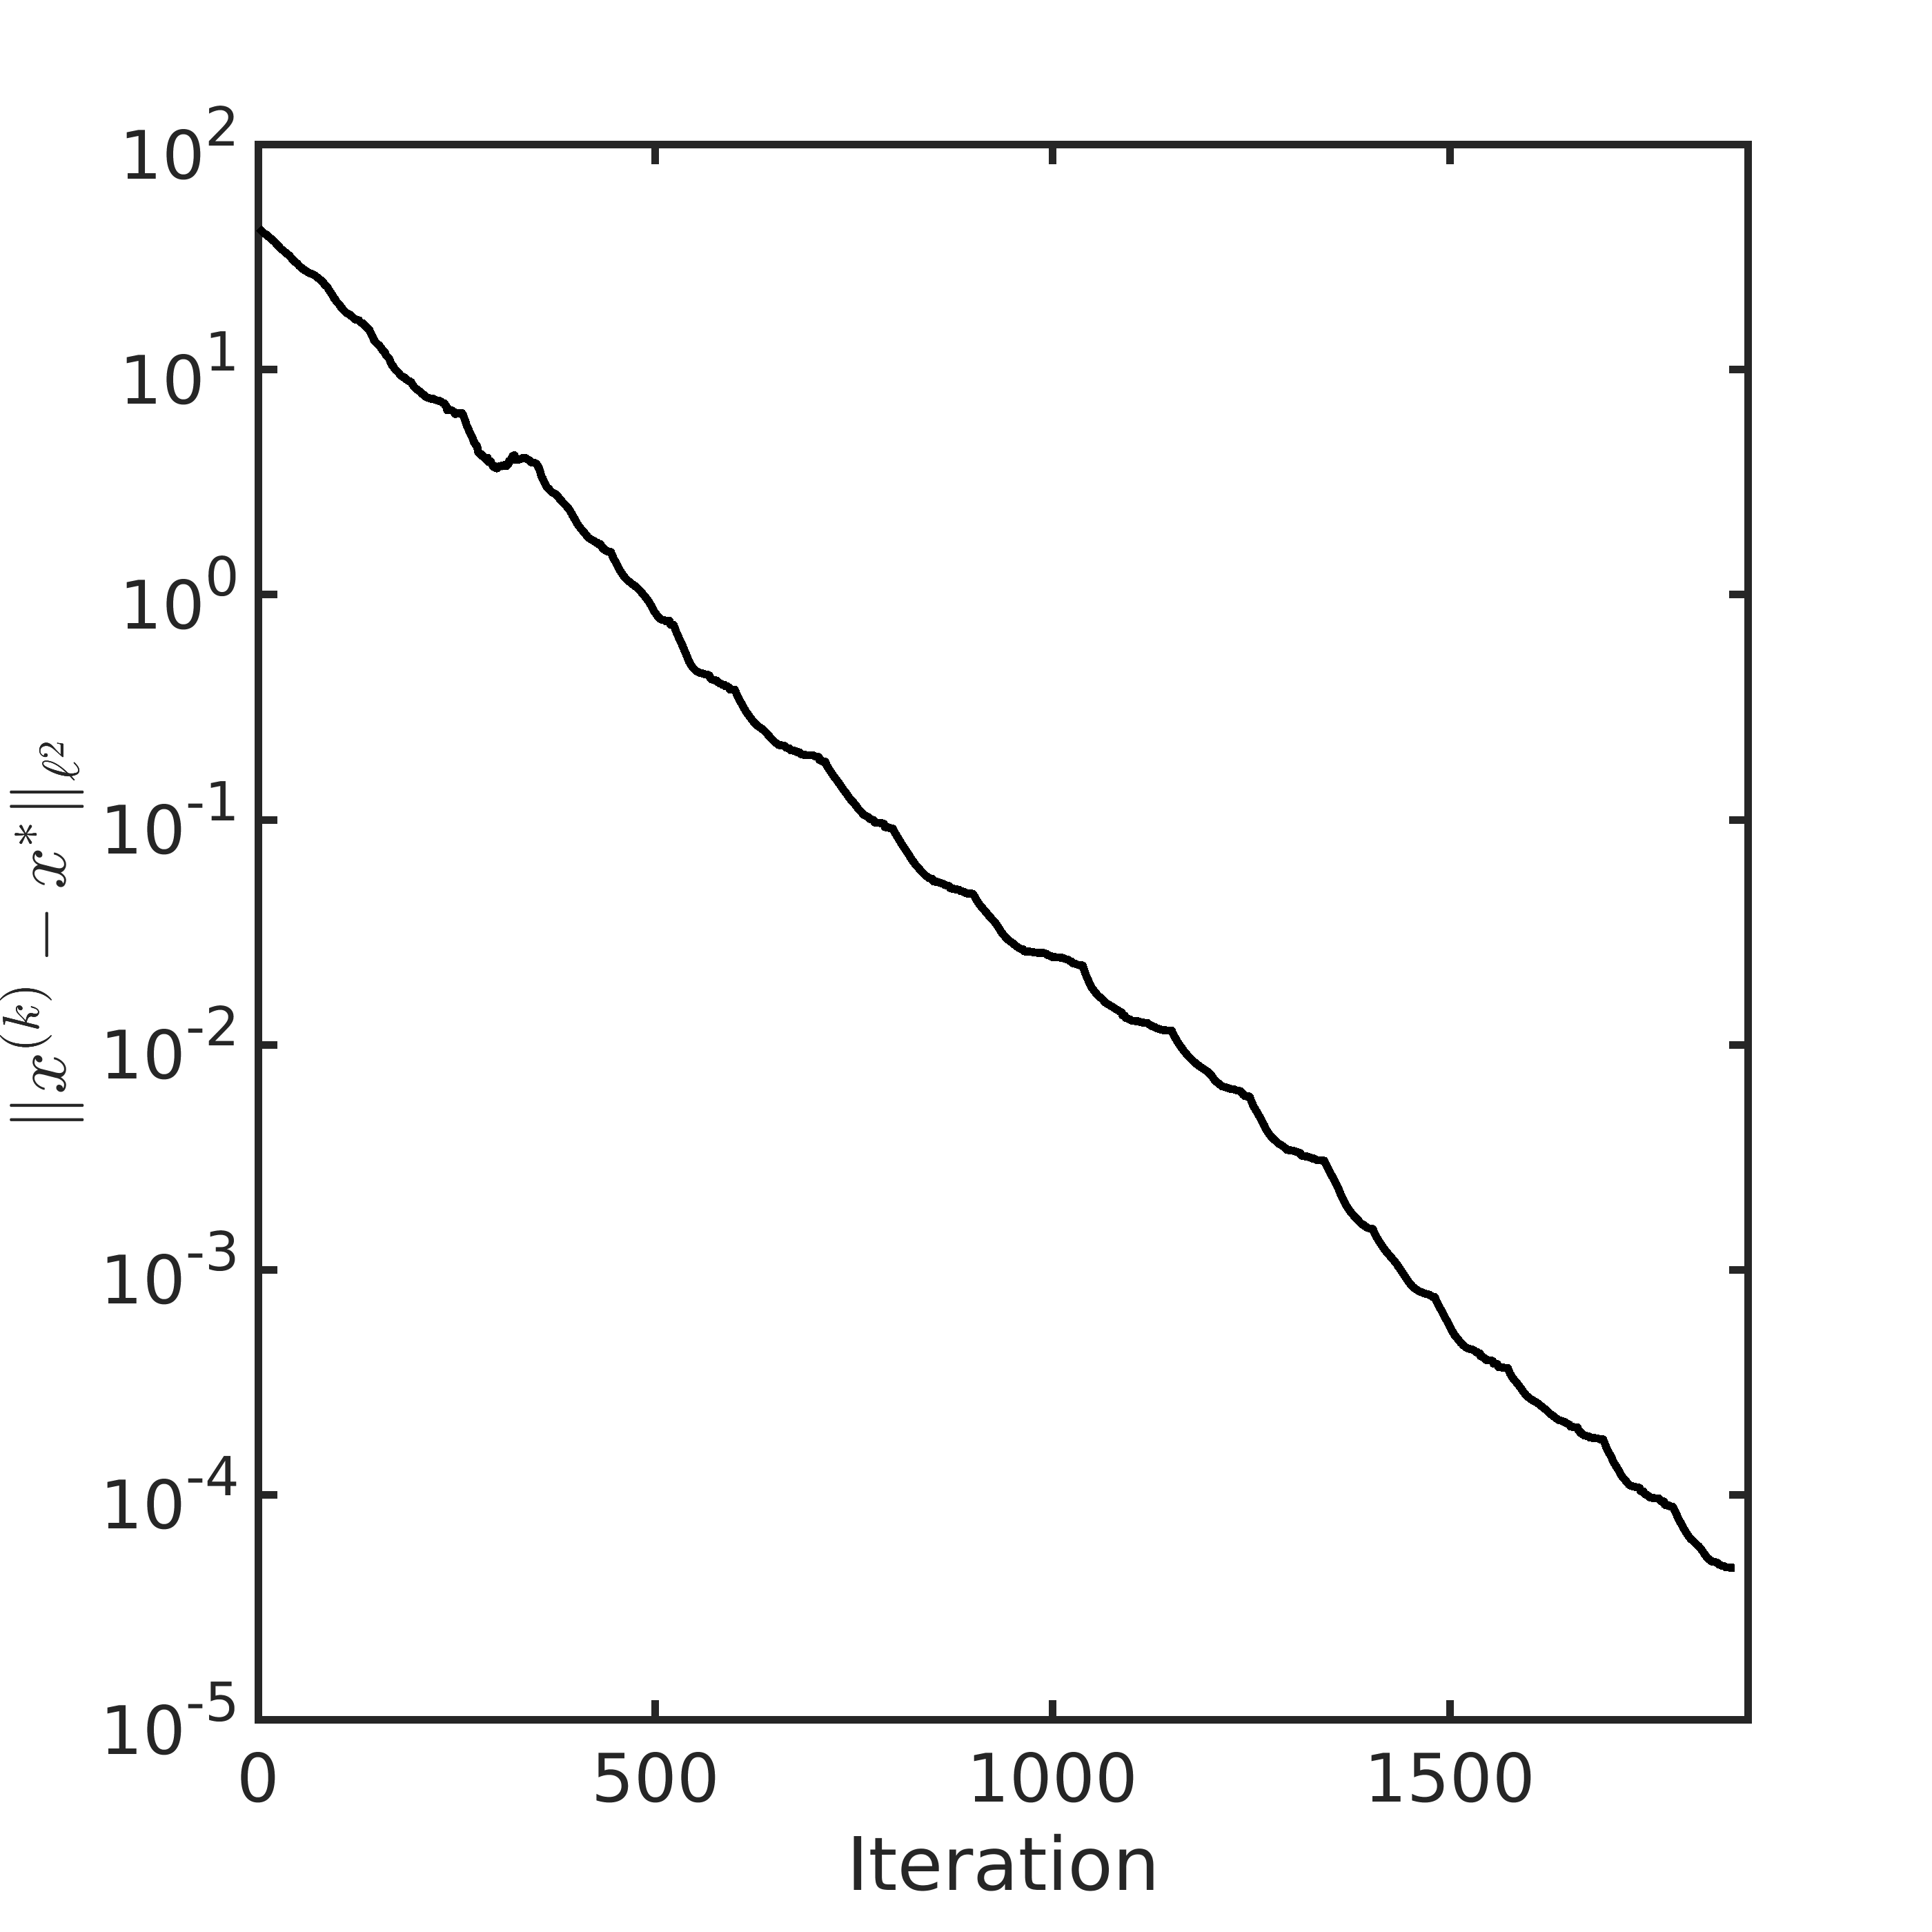
\includegraphics[scale=0.25]{../figures/ackley100D_dist.png}
%      \caption{The iteration process of the adaptive HiCS method to the $100$
%      dimensional Ackley function when the HiCS algorithm is
%      convergent with initial search radius $\rho=2.0$ and the random
%      initial value generated in $[-5,5]^{100}$.}
%      \label{fig:ackley100D:AHiCS}
%\end{figure}
%
%
%Then we try to test the ability of the proposed method for 
%approximating different minimizer of the Ackley function.
%Since the unique parameter in the HiCS algorithm is the
%search radius. 
%We carry out the adaptive HiCS method $30$ times using different 
%initial search radius $\rho_0$. The initial value is generated
%randomly in the region of $[-5,5]^{100}$. 
%The convergent criterion is the $\ell^2$-distance between the
%convergent SMP and the global minimizer smaller than
%$\varepsilon=10^{-14}$.
%Fig.\,\ref{fig:ackley100D:AHiCS:randinit} gives the 
%$\ell^2$-distance, and
%the function value after convergence when $\rho_0=0.05, 0.1, 0.5$,
%and $0.8$, respectively. Obviously, with the increment of $\rho_0$,
%the convergent point is close to the global minimizer in the
%average sense. Correspondingly, the convergent function value
%becomes small. It can be found that when $\rho_0=0.8$, the adaptive
%HiCS method can find the neighbourhood with radius $10^{-14}$ of the
%global minimizer $0$ for several times. 
%It demonstrates that the adaptive HiCS method can capture the global minimizer
%if $\rho_0$ is appropriately increased. 
%
%\begin{figure}[!htbp]
%    \begin{minipage}[b]{0.5\linewidth}
%    \centering{
%      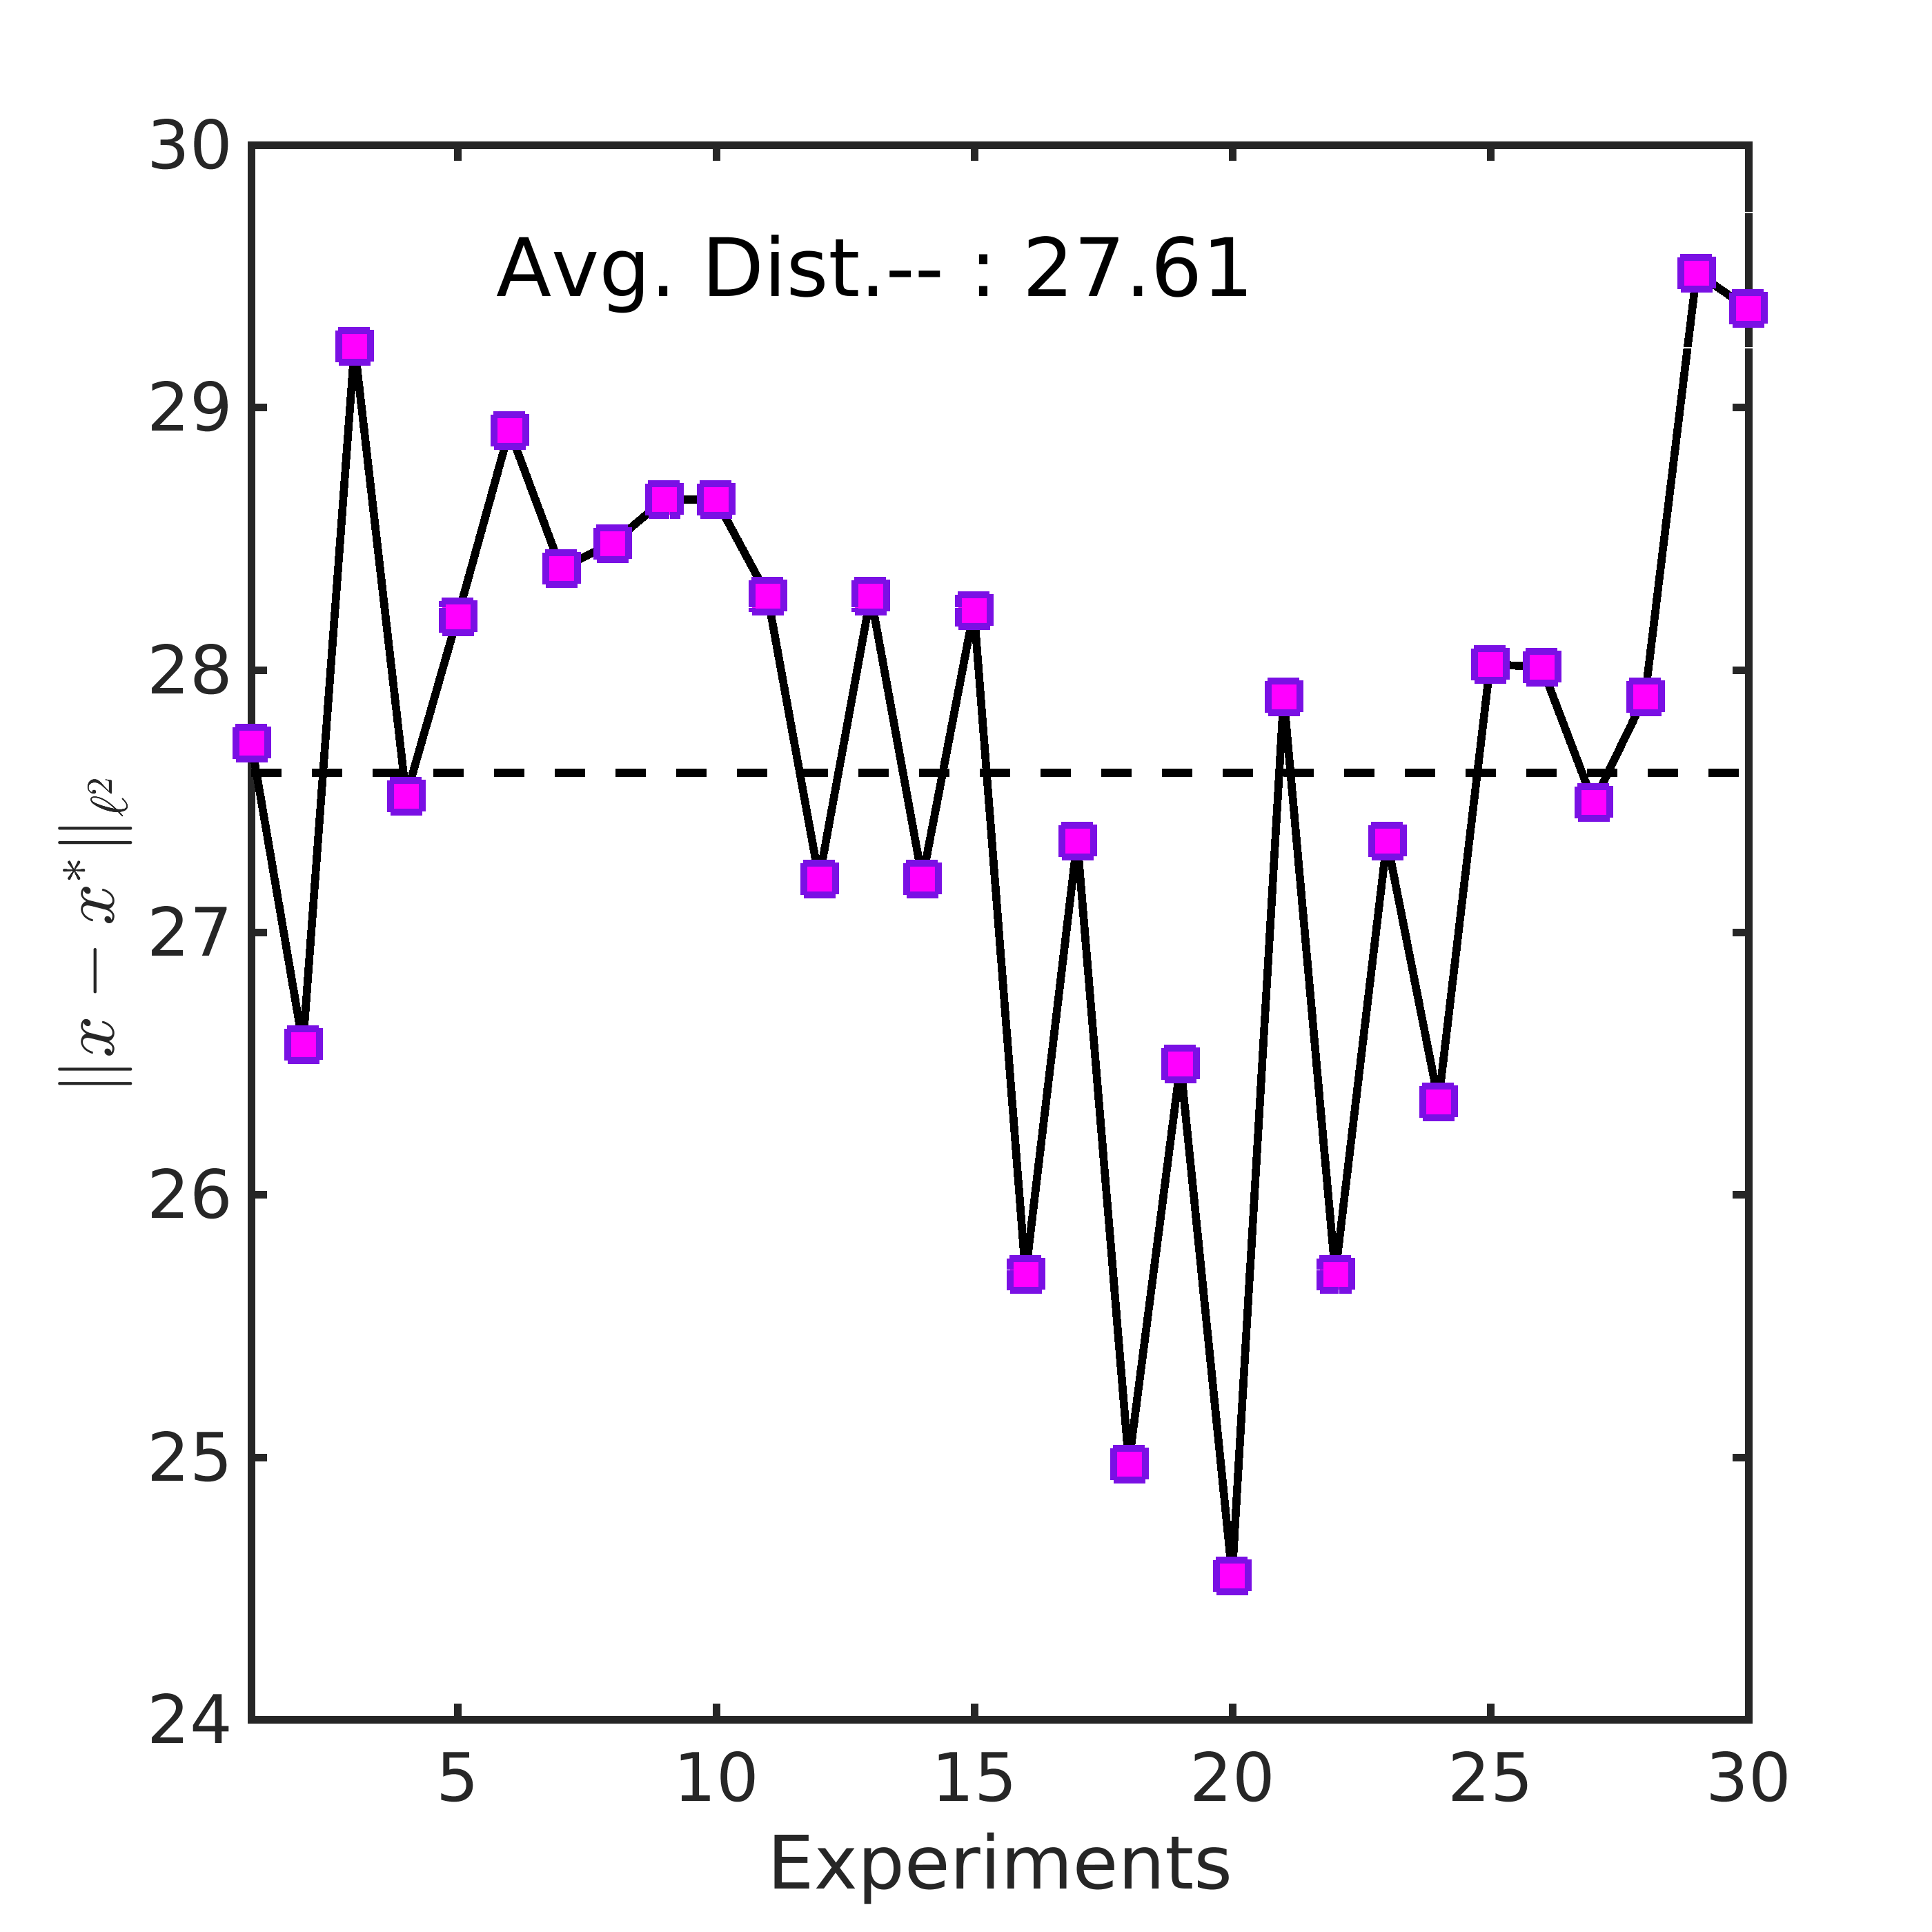
\includegraphics[scale=0.125]{../figures/ackley100Drandr0_05_dist.png}
%      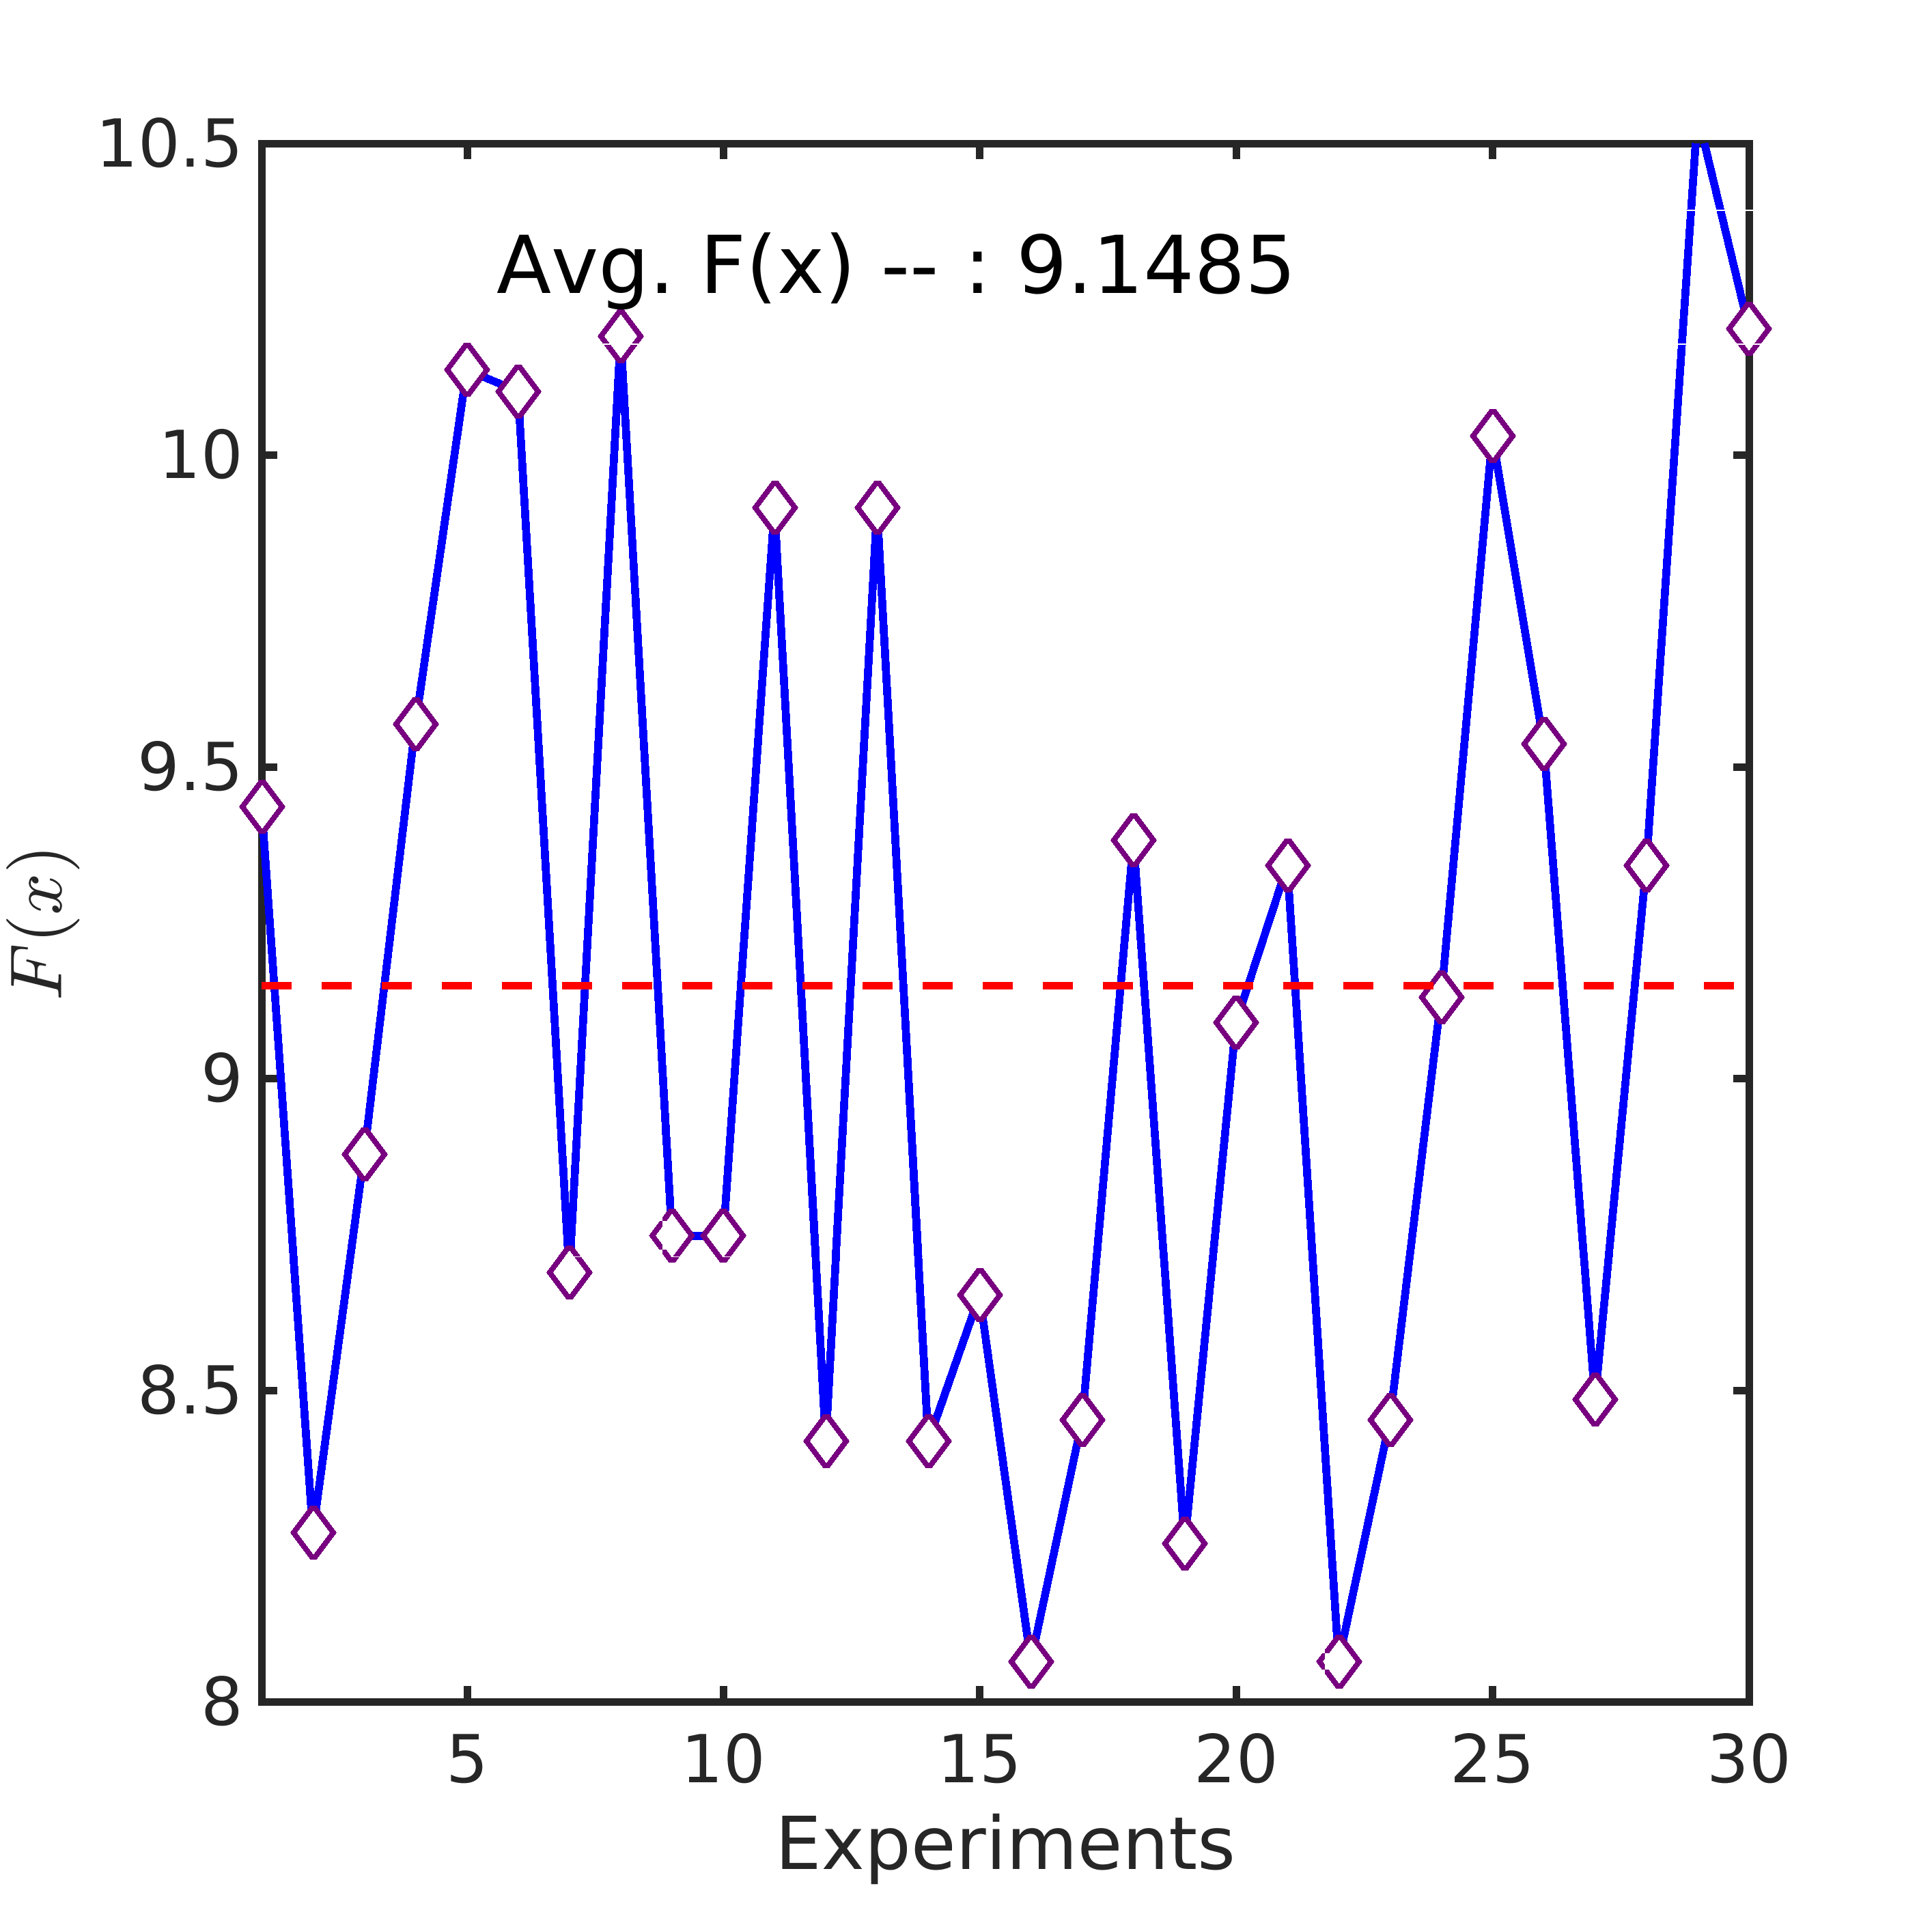
\includegraphics[scale=0.125]{../figures/ackley100Drandr0_05_val.png}
%      }
%    \centerline{(a) $\rho_0 =0.05$}
%    \end{minipage}
%    %%%%%%%
%    \begin{minipage}[b]{0.5\linewidth}
%    \centering{
%      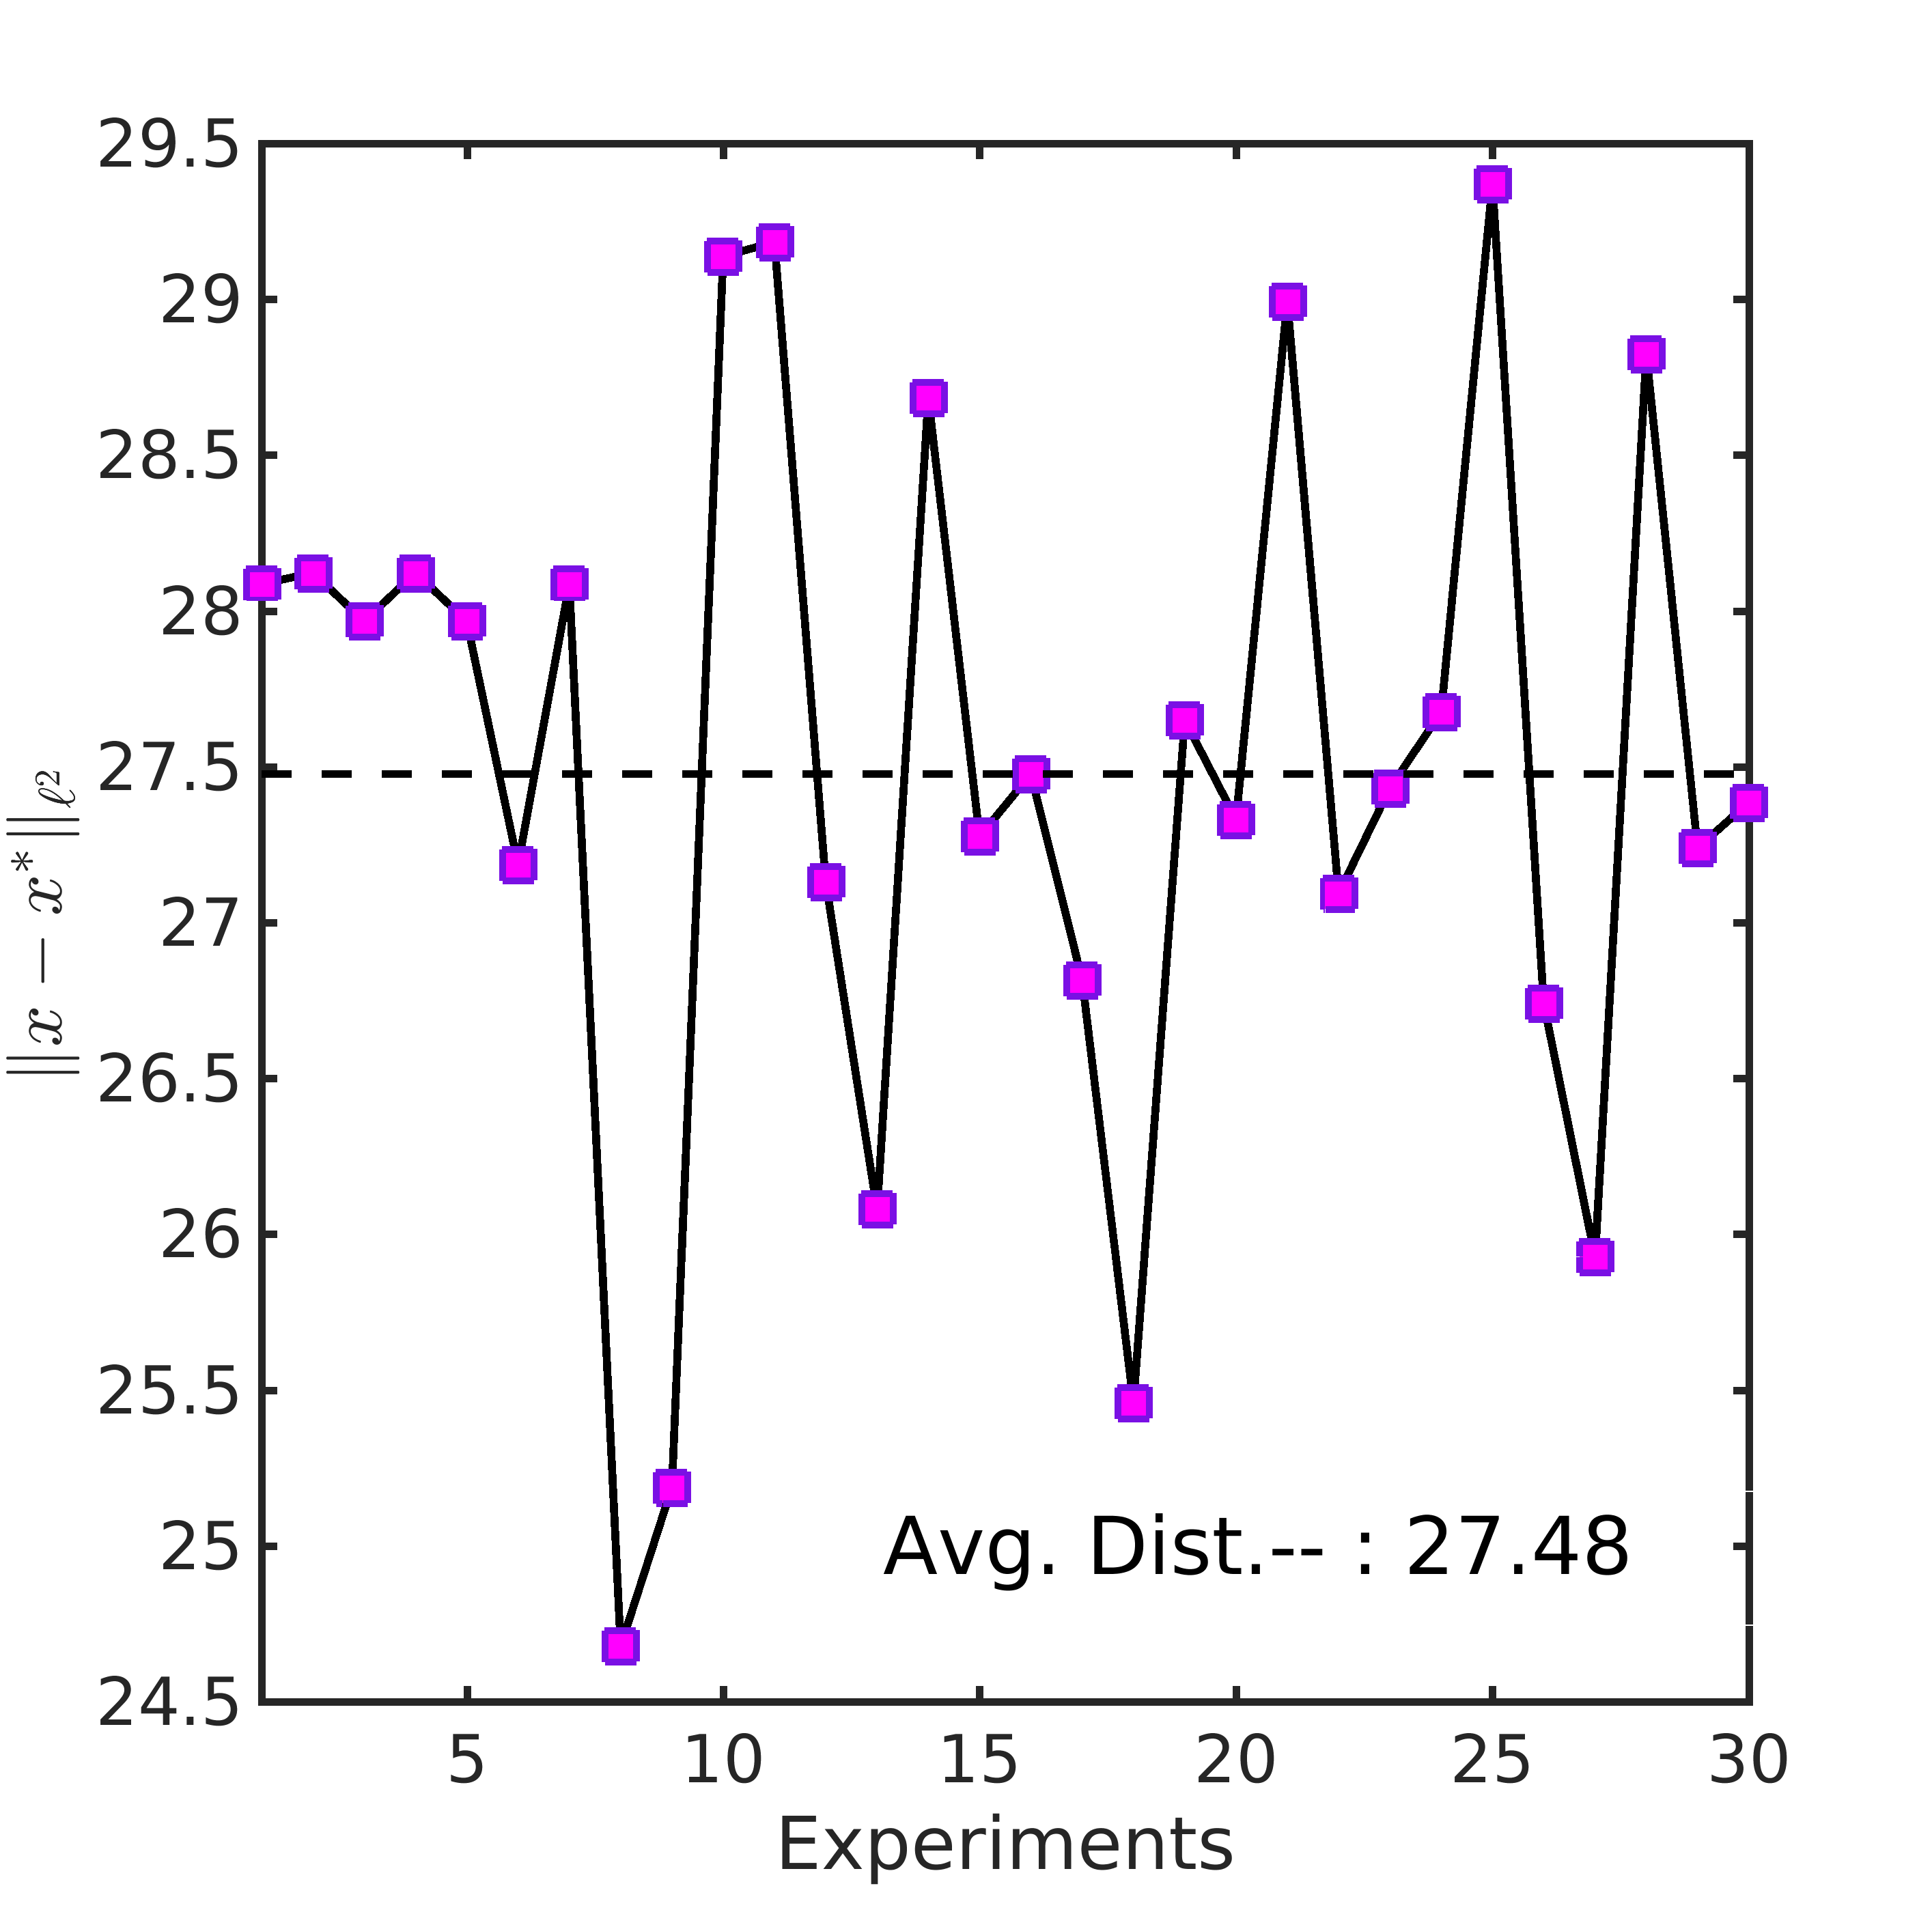
\includegraphics[scale=0.125]{../figures/ackley100Drandr0_1_dist.png}
%      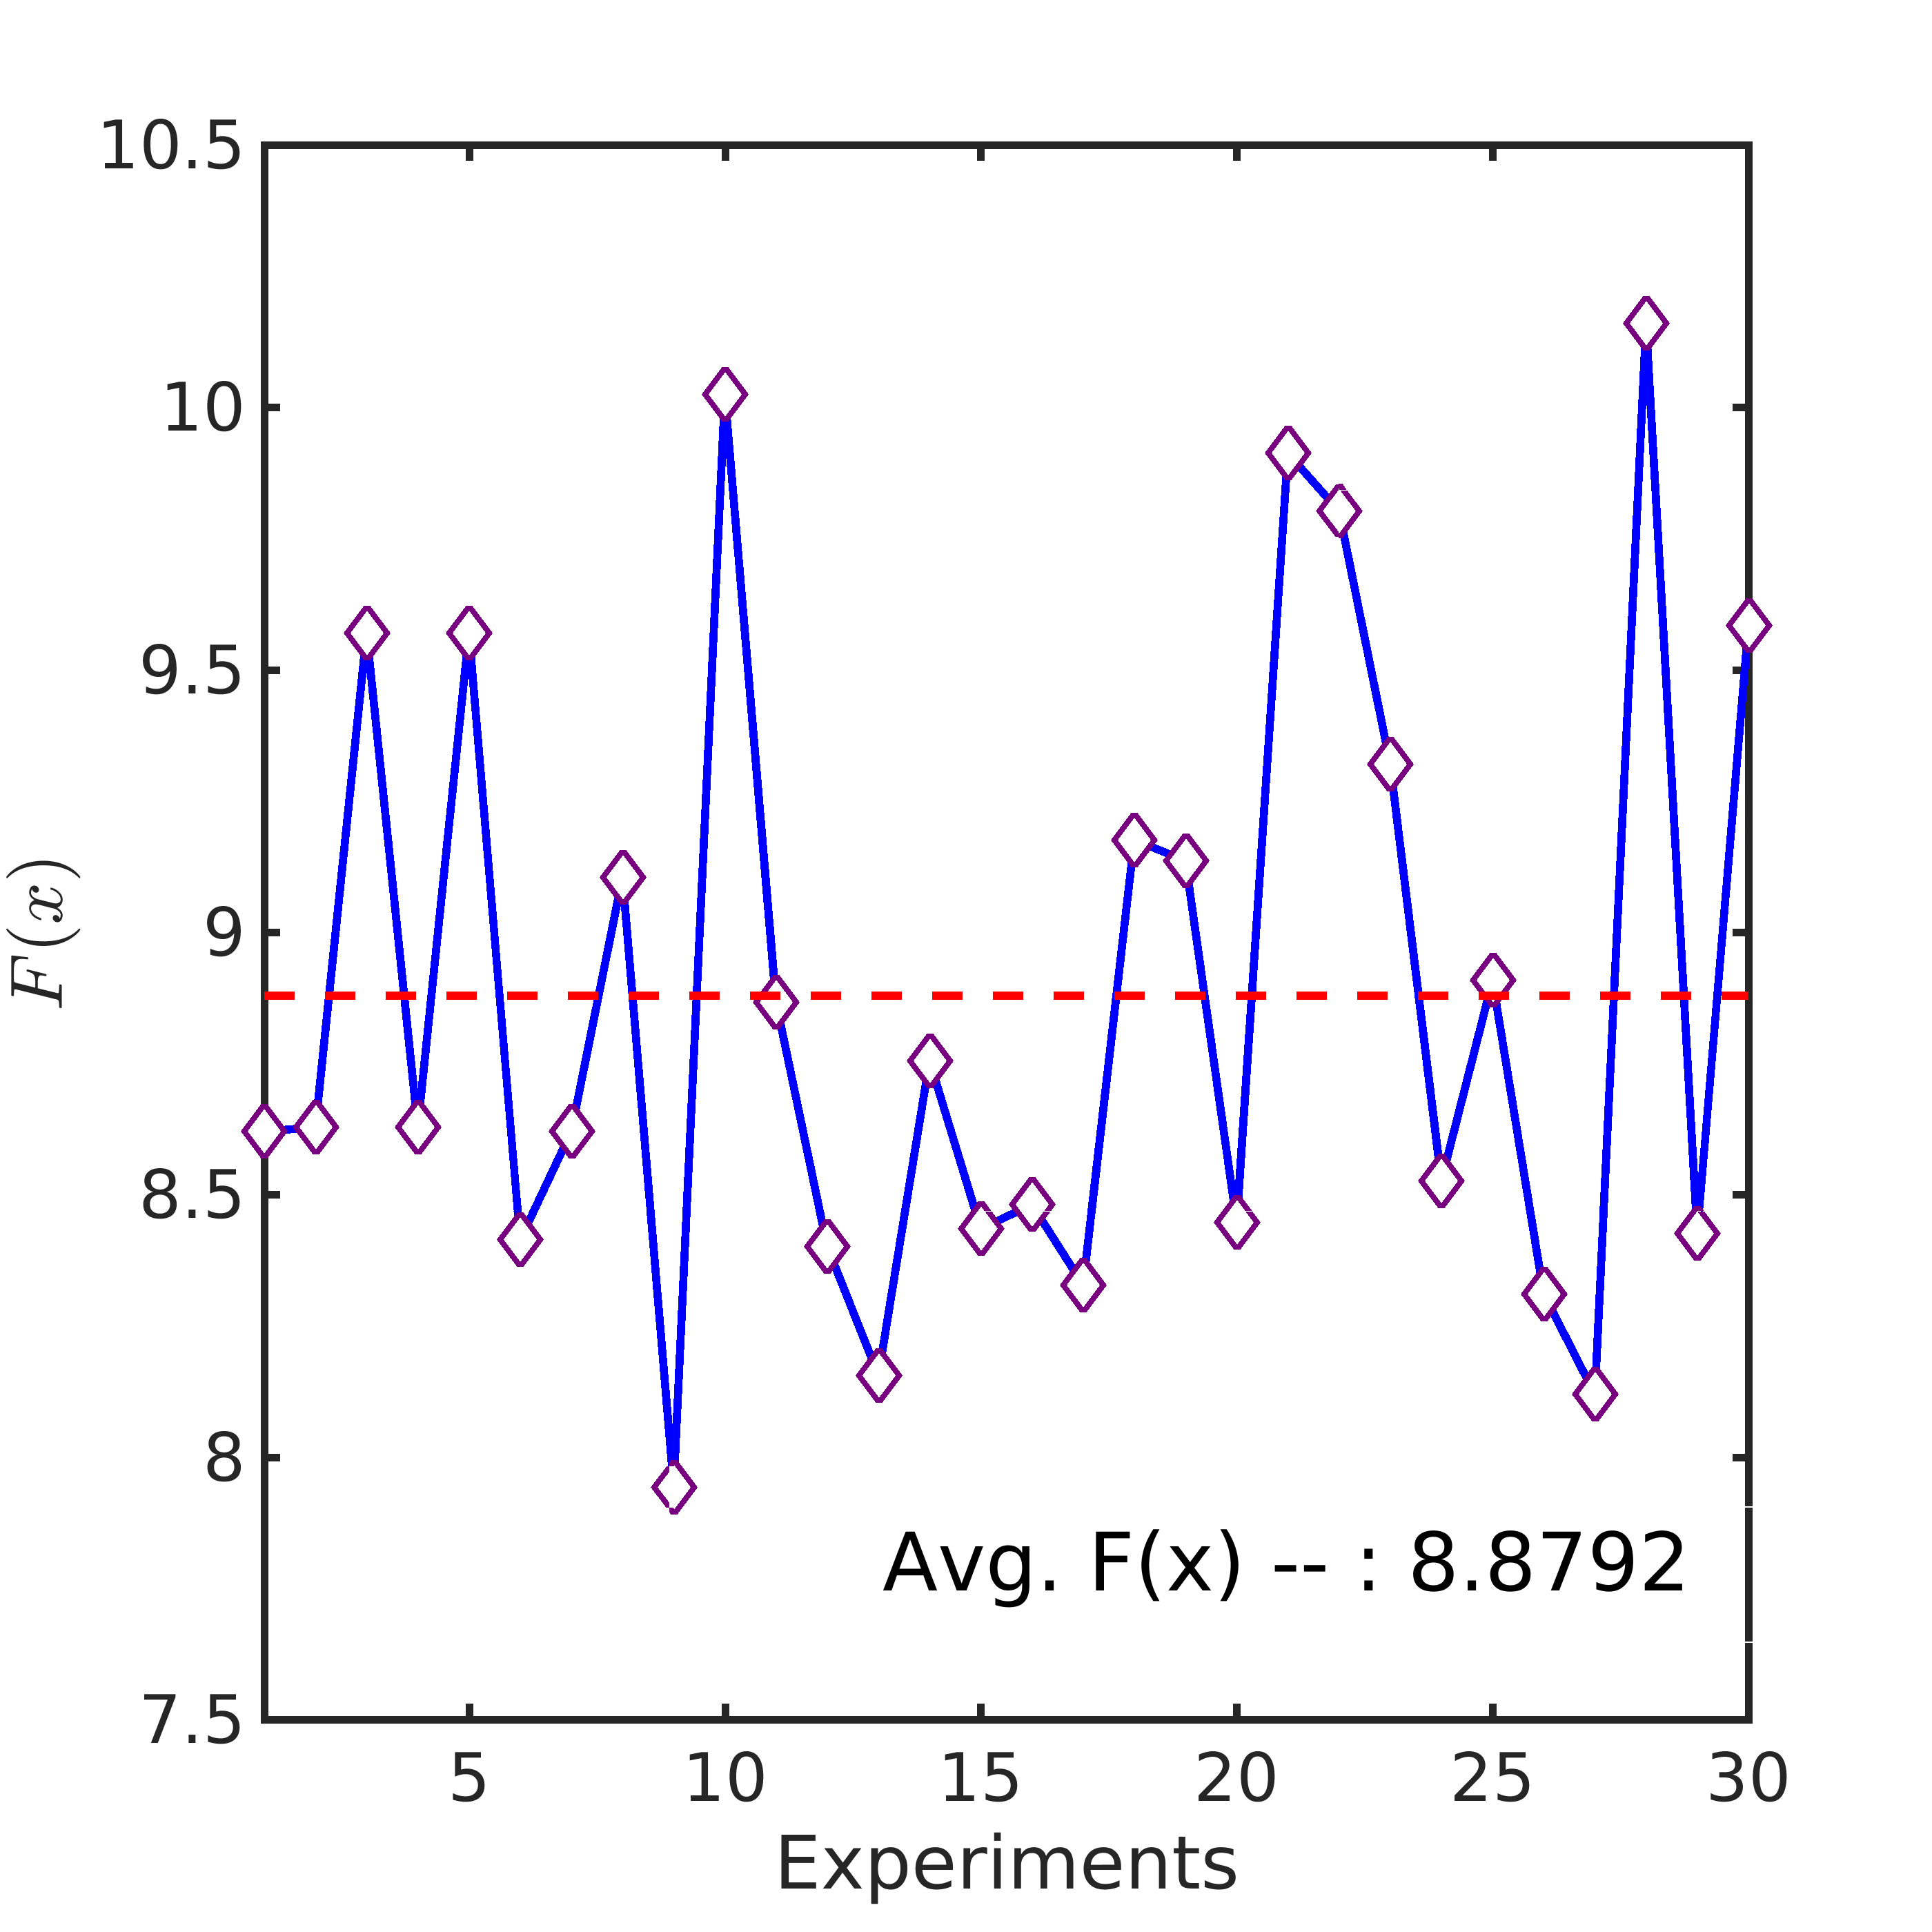
\includegraphics[scale=0.125]{../figures/ackley100Drandr0_1_val.png}
%      }
%    \centerline{(b) $\rho_0=0.1$}
%    \end{minipage}
%    %%%%%%%
%    \begin{minipage}[b]{0.5\linewidth}
%    \centering{
%      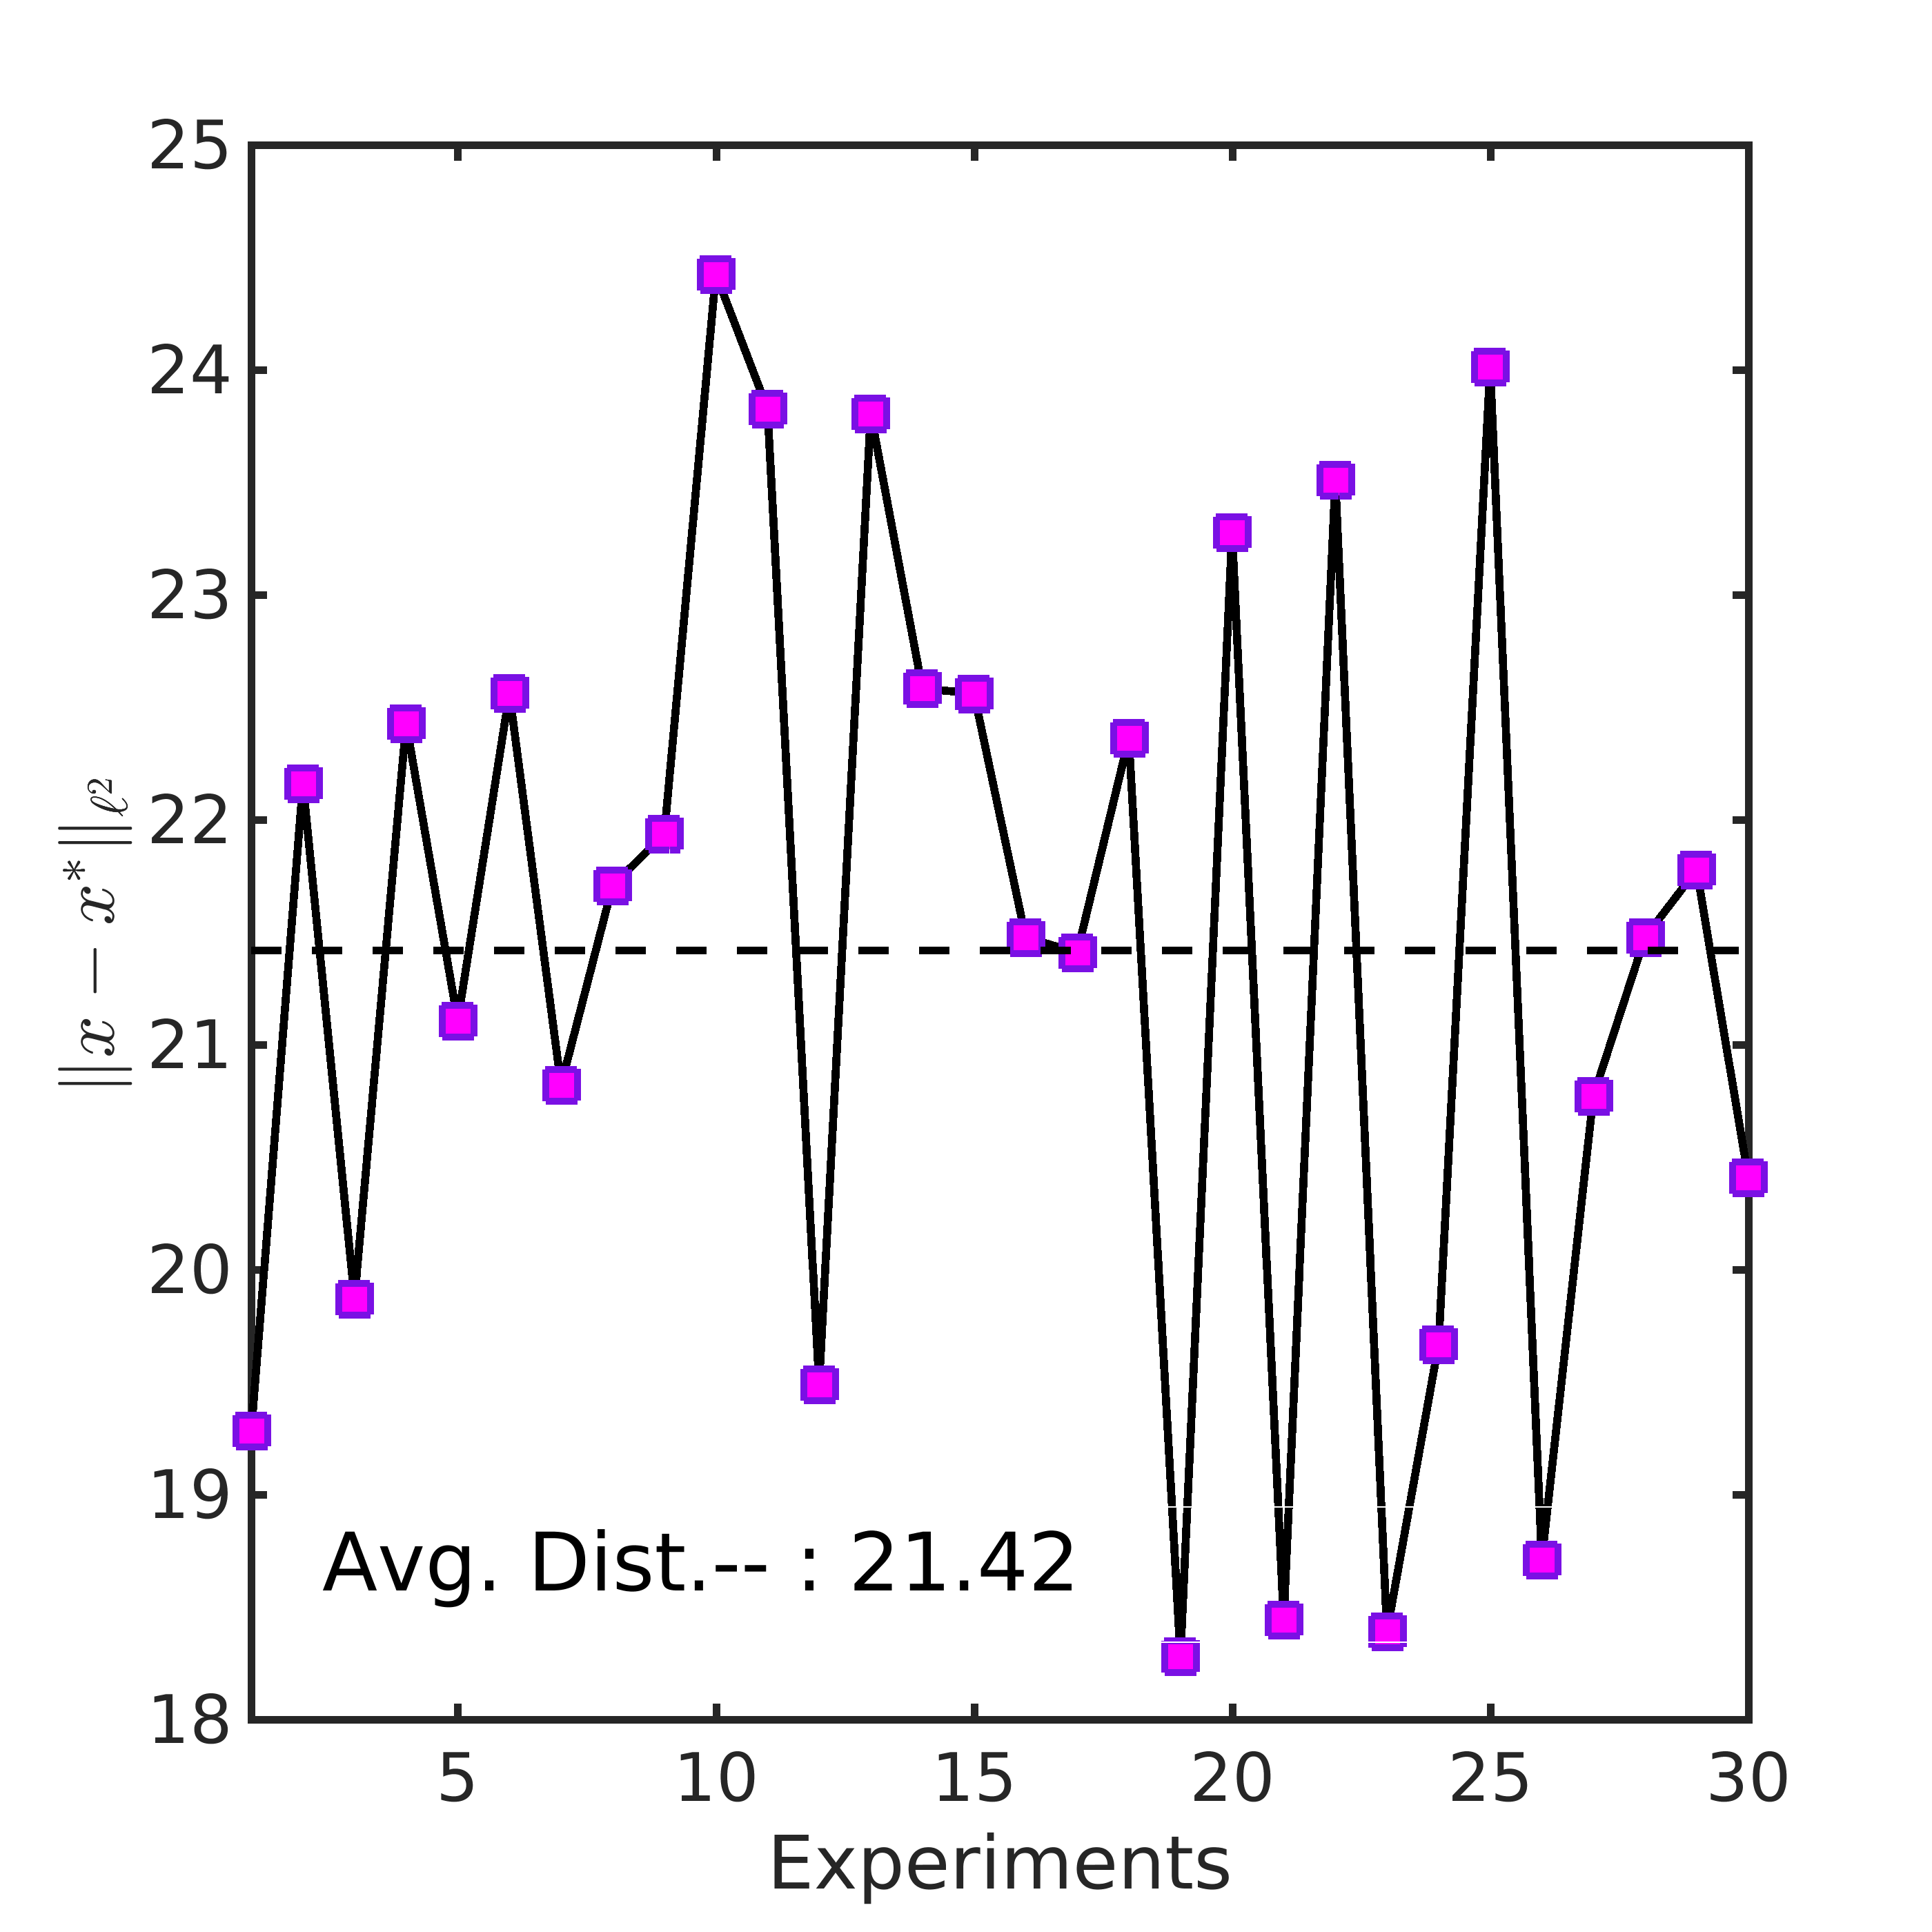
\includegraphics[scale=0.125]{../figures/ackley100Drandr0_5_dist.png}
%      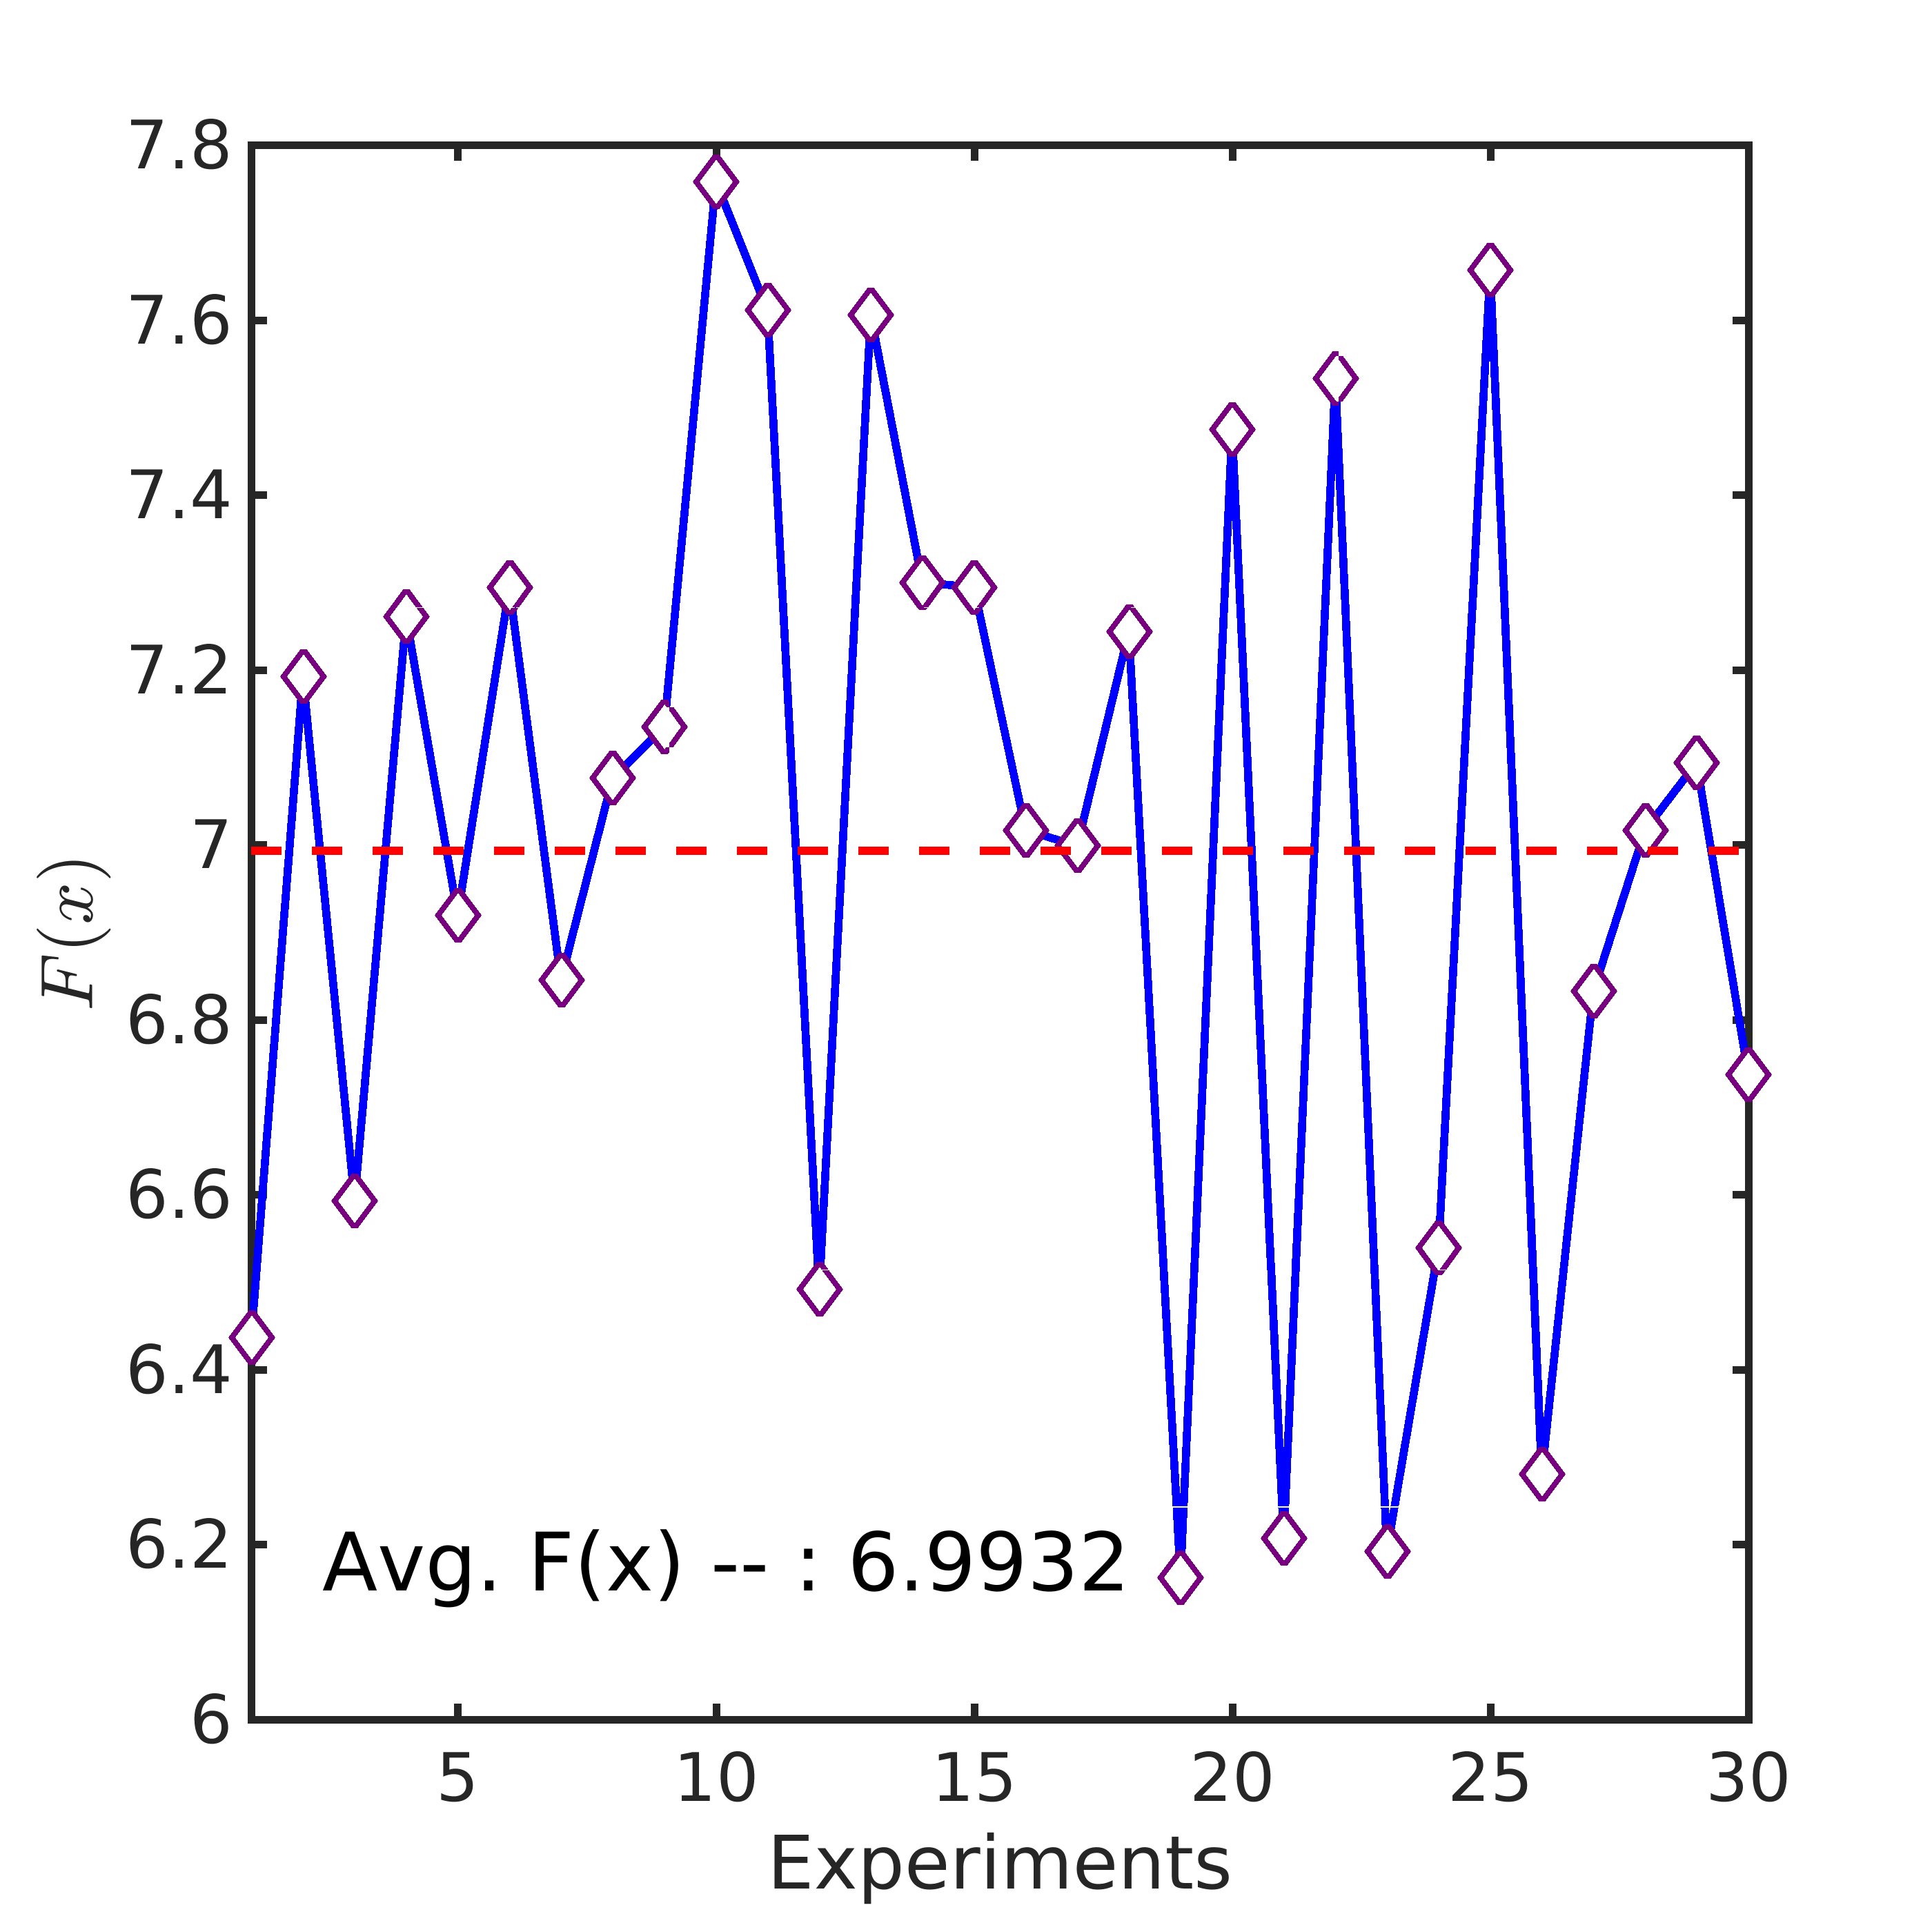
\includegraphics[scale=0.125]{../figures/ackley100Drandr0_5_val.png}
%      }
%    \centerline{(c) $\rho_0 =0.5$}
%    \end{minipage}
%    %%%%%%%
%    \begin{minipage}[b]{0.5\linewidth}
%    \centering{
%      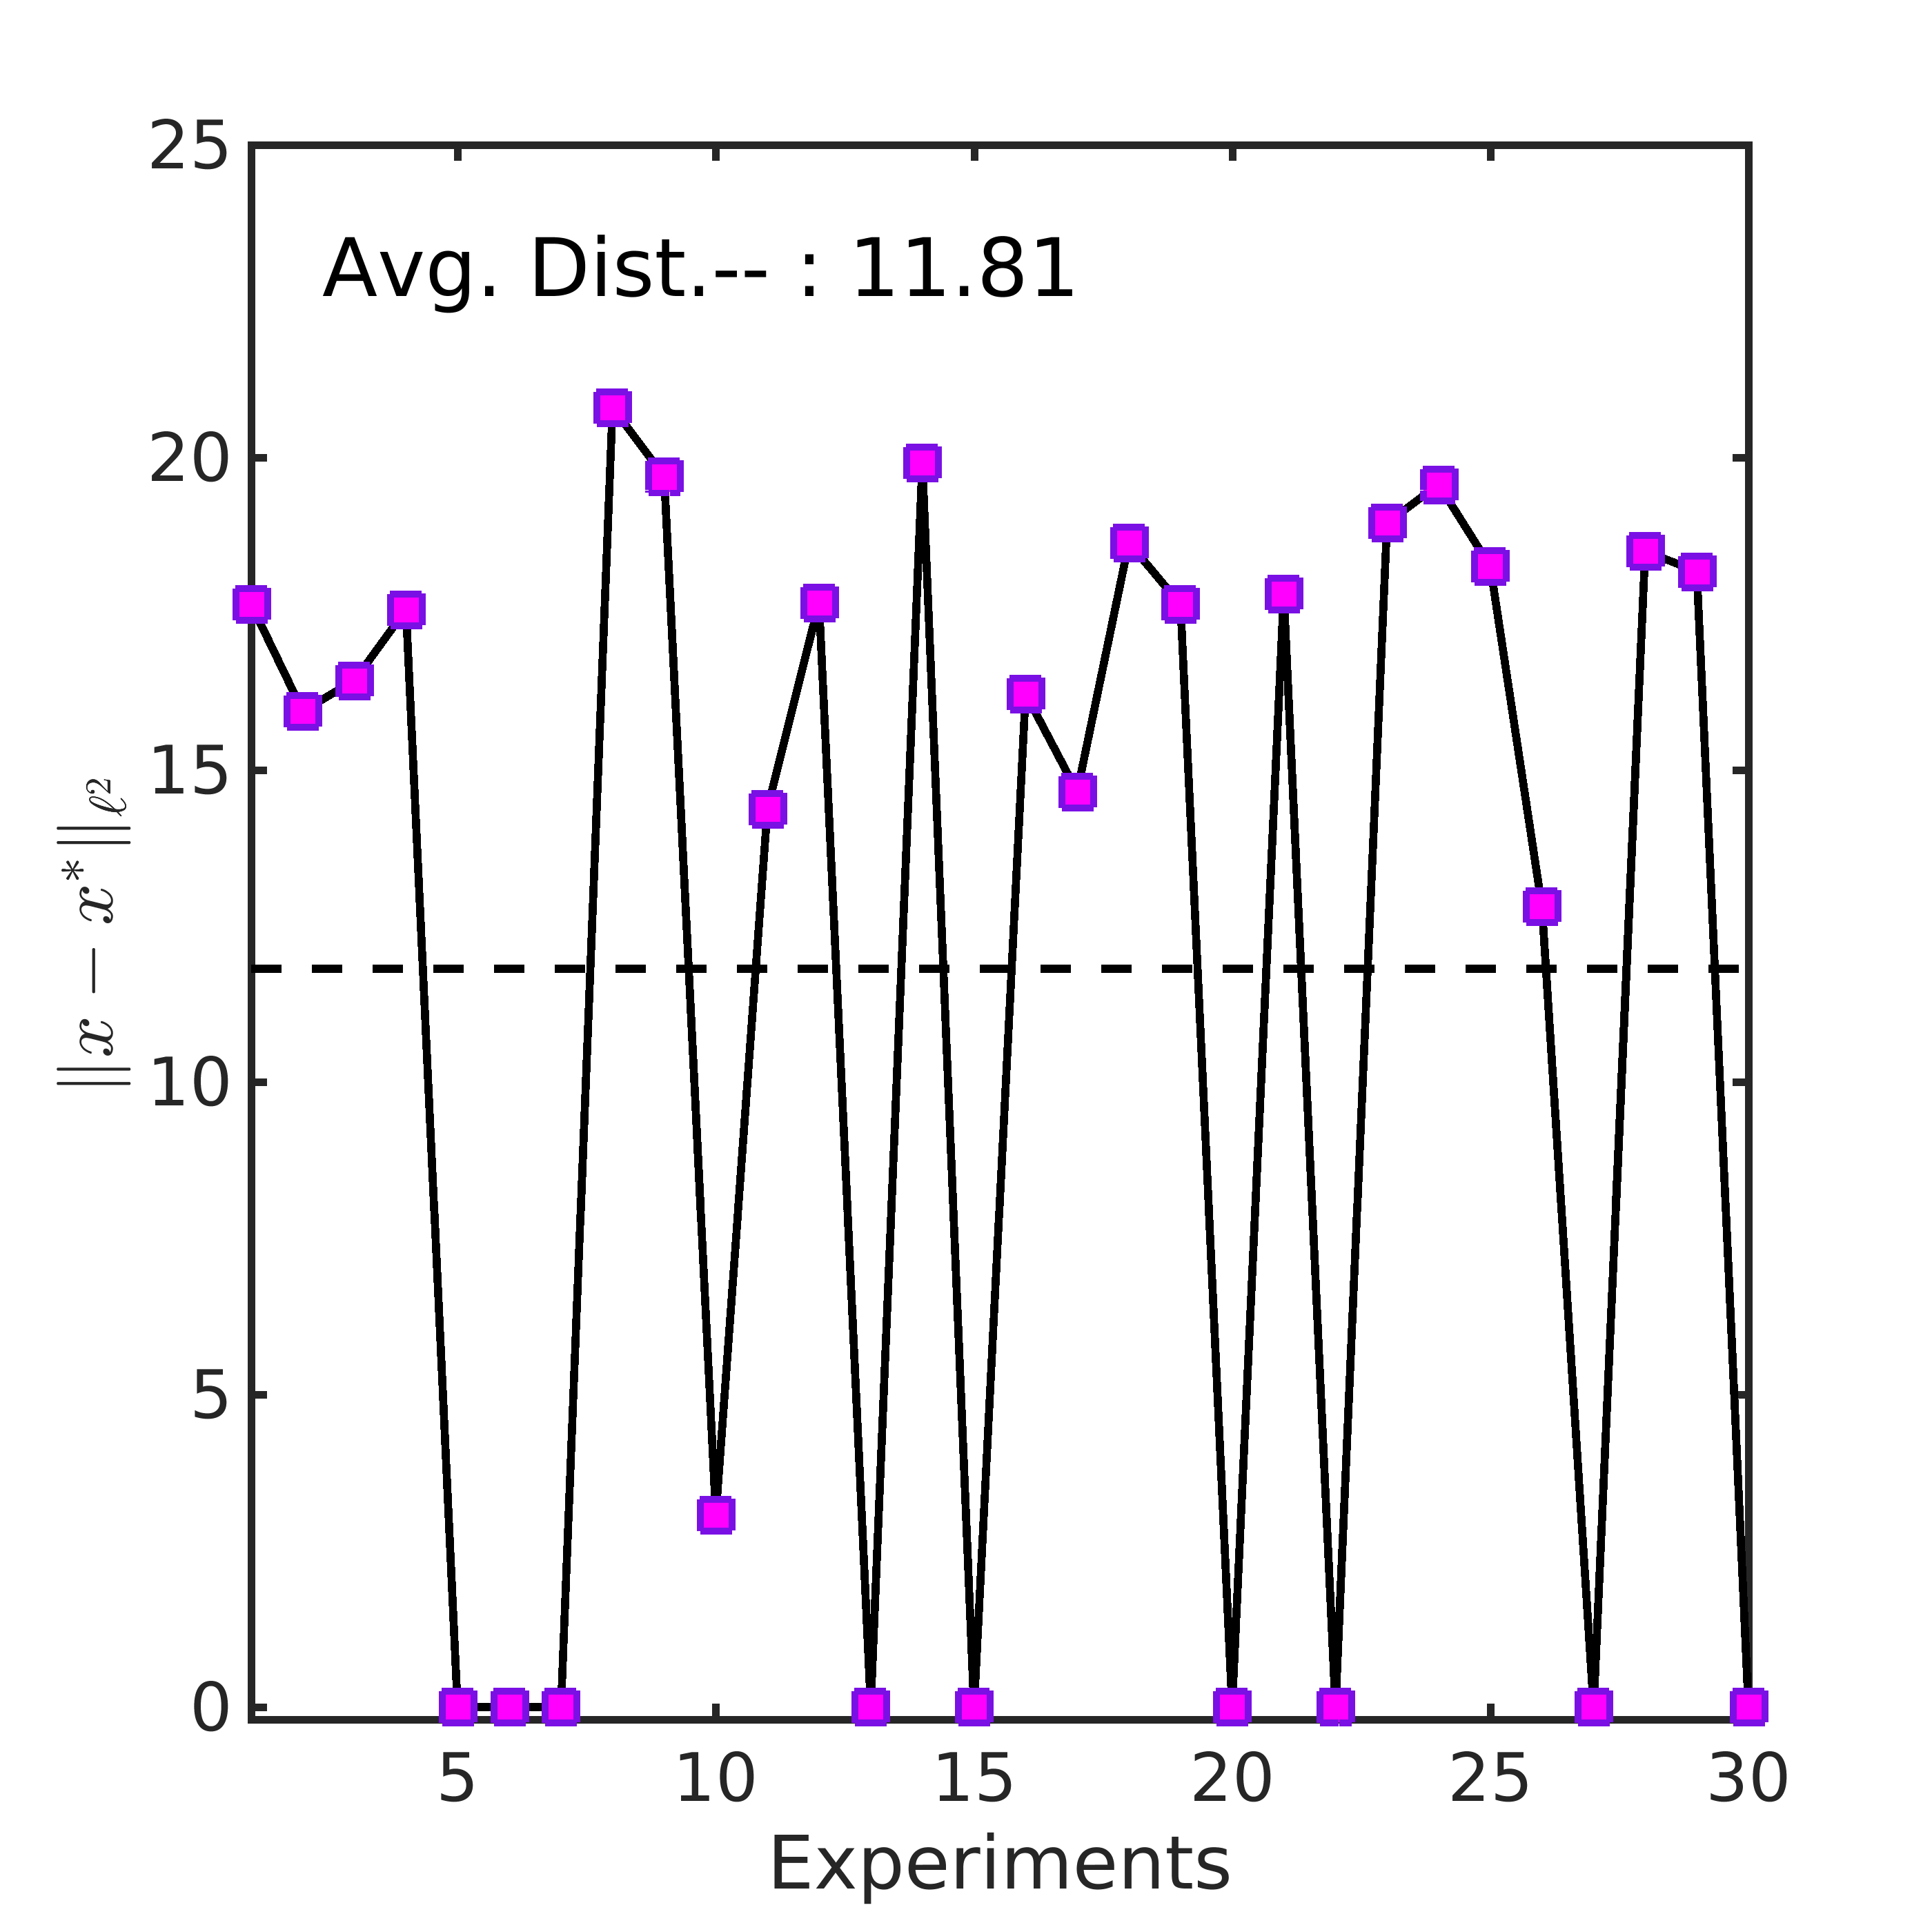
\includegraphics[scale=0.125]{../figures/ackley100Drandr0_8_dist.png}
%      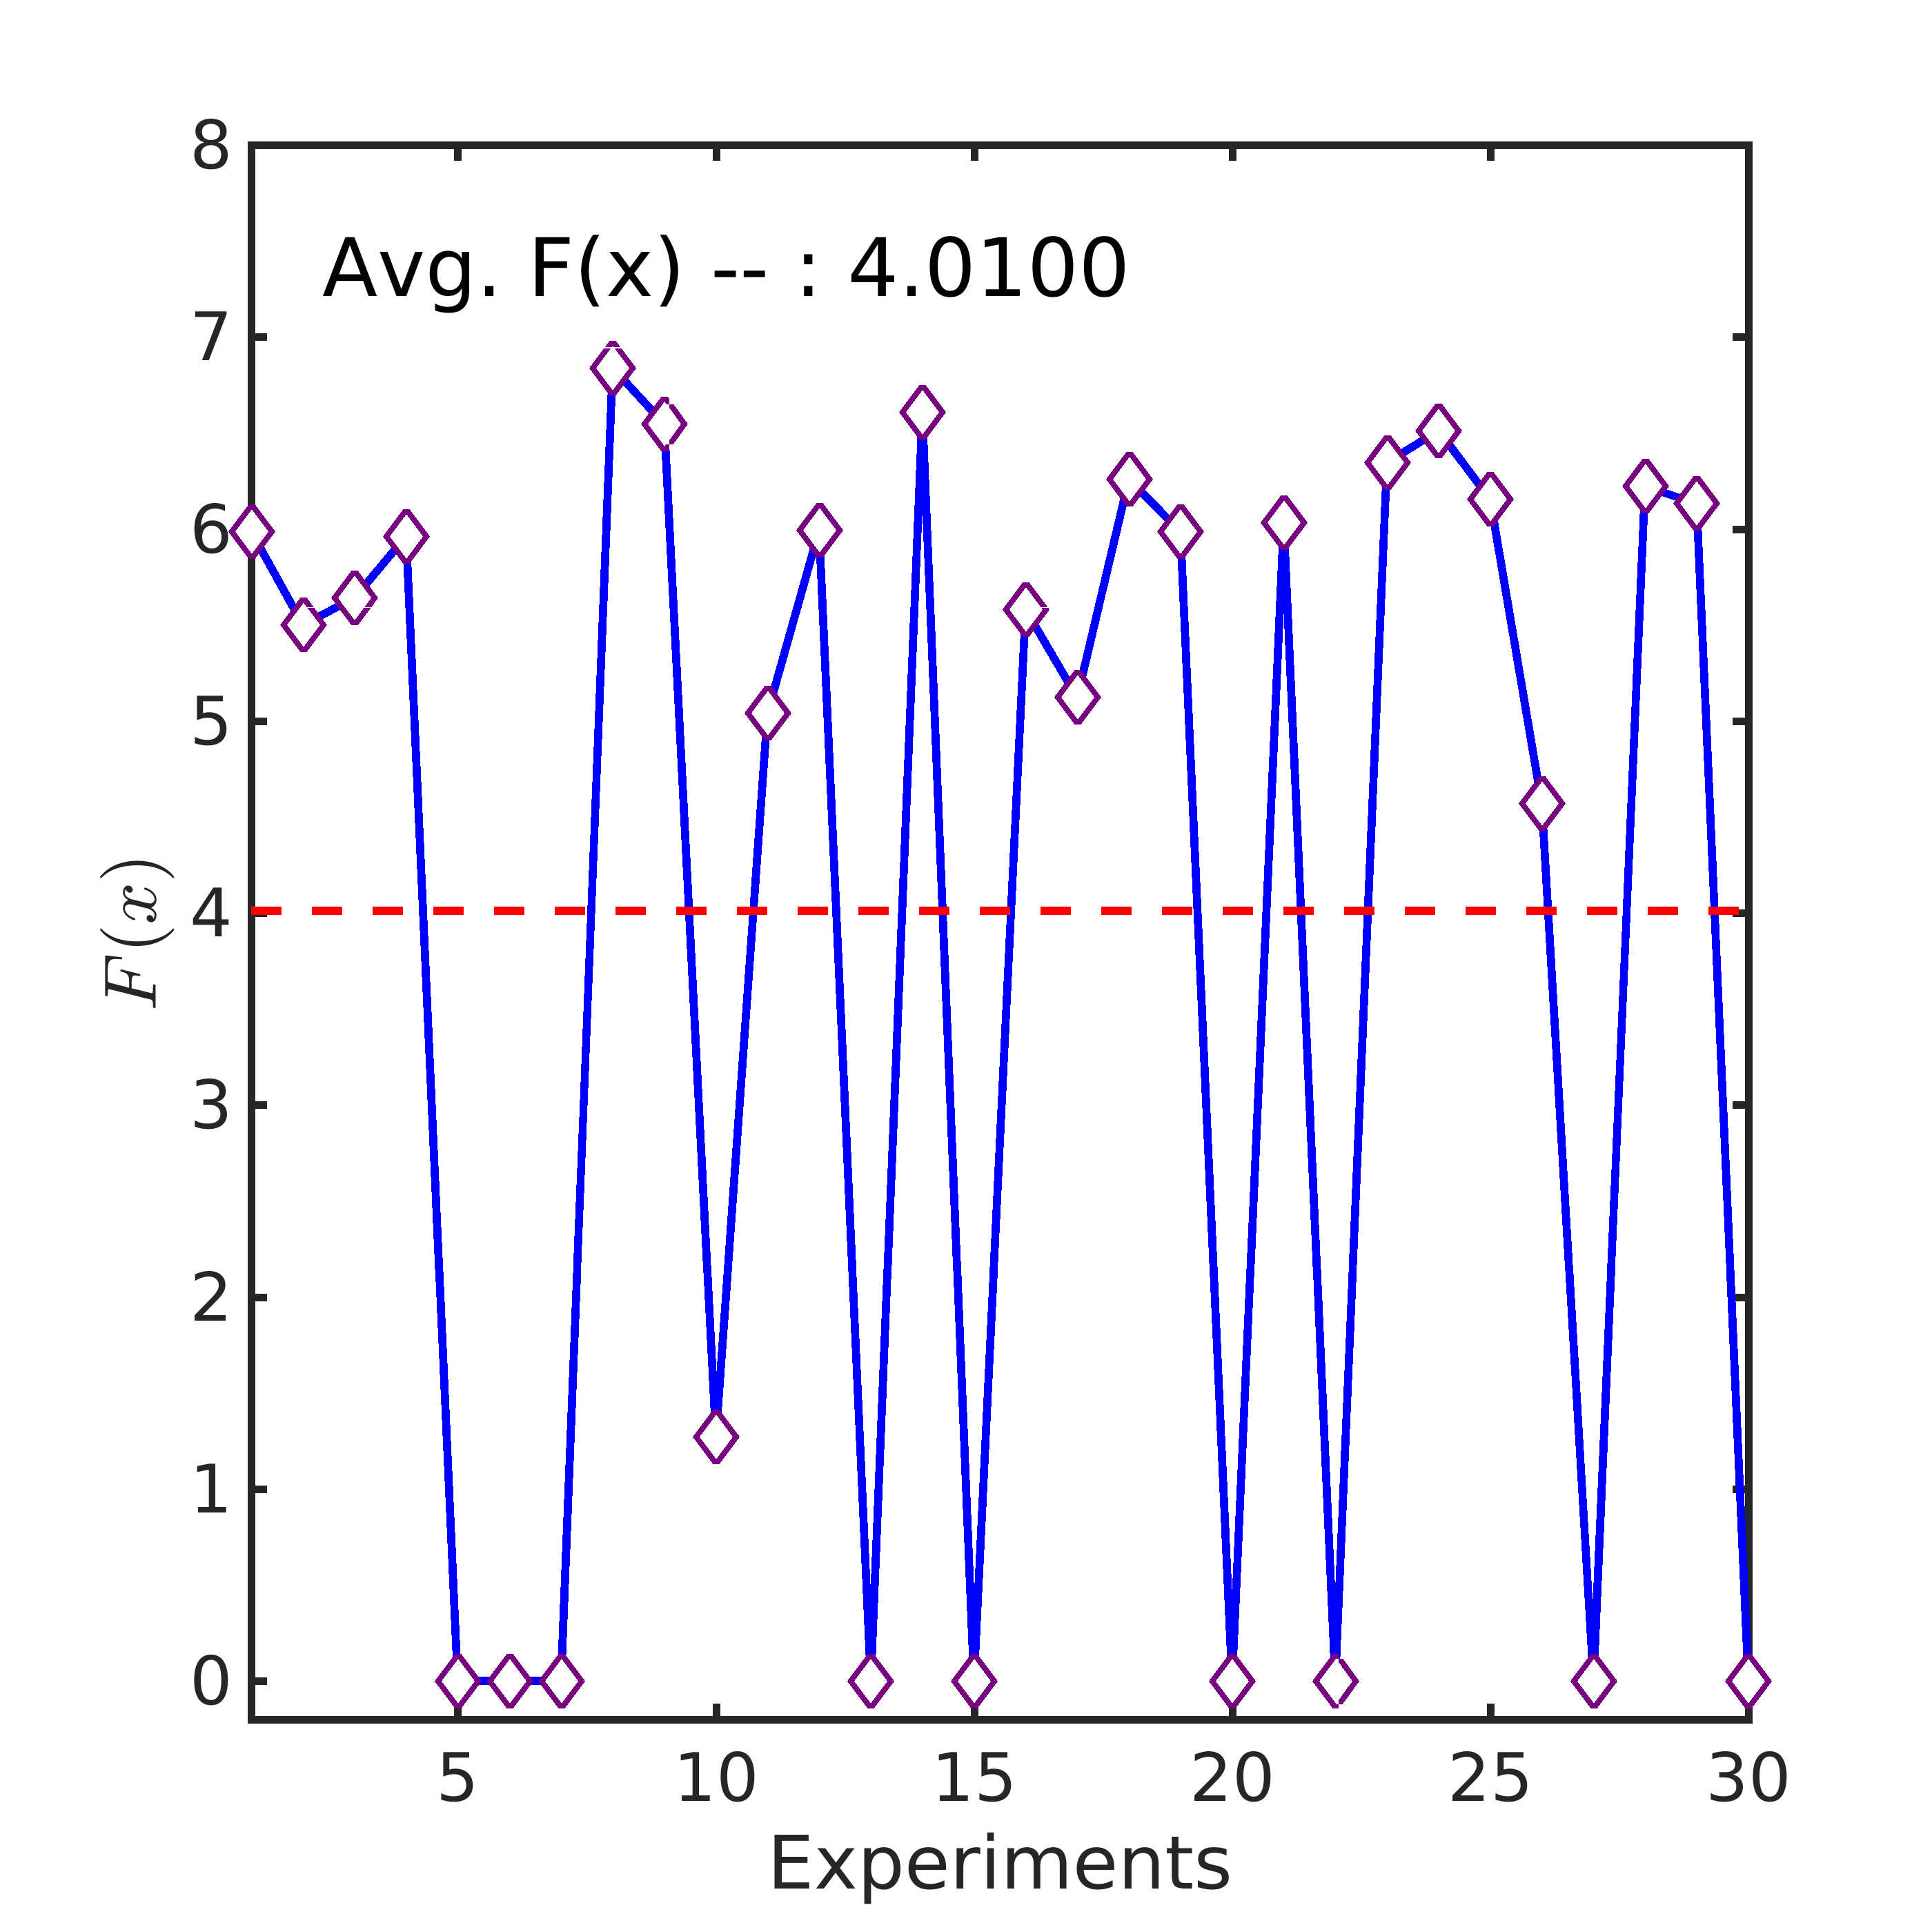
\includegraphics[scale=0.125]{../figures/ackley100Drandr0_8_val.png}
%      }
%    \centerline{(d) $\rho_0 =0.8$}
%    \end{minipage}
%    %%%%%%%
%      \caption{The iteration process of the adaptive HiCS method to 100
%      dimensional Ackley function with different initial search
%      radius $\rho_0$. Start point is randomly generated in the
%      space $[-5, 5]^{100}$. } 
%      \label{fig:ackley100D:AHiCS:randinit}
%\end{figure}
%
We continue to apply the adaptive HiCS method to $2500$ dimensional
Ackley function. The initial search radius is $\rho_0=3.5$, and
the initial position is generated randomly in $[-10,10]^{2500}$. 
The iteration process is presented in Fig.\,\ref{fig:ackley2500D:AHiCS}. 
For such a high dimensional optimization problem, the iteration
behavior is similar to previous numerical experiments. 
When $\rho=3.5$, the HiCS method costs $90$ steps to achieve convergence.
By further shrinking search radius, the adaptive HiCS can
capture global minimizer. As one can see from 
Fig\,\ref{fig:ackley2500D:AHiCS}, the global minimizer always
locates in the search neighbourhood in this case. 
It demonstrates that the HiCS has the capacity of hupping the
local basin even for such a high dimensional problem.
%It costs roughly $3.7$ hours of real time using one Inter 3.60 GHz i7-4790 processor.
\begin{figure}[!htbp] 
	\centering
	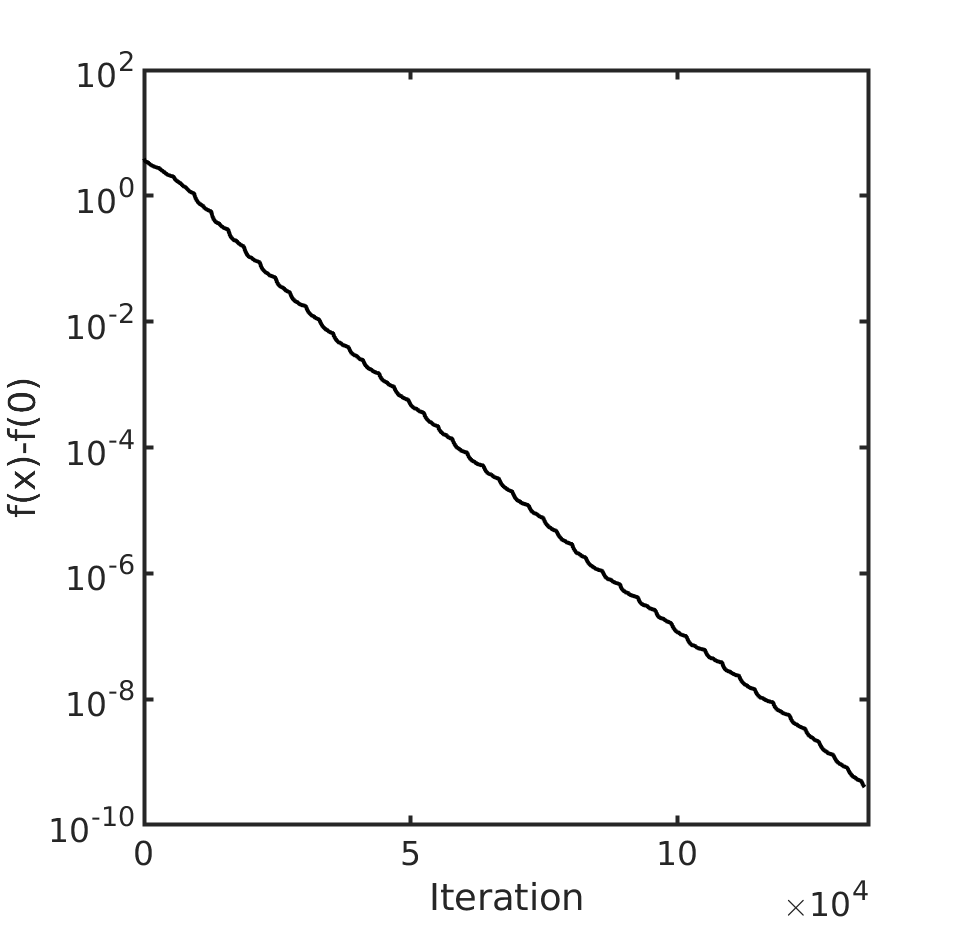
\includegraphics[scale=0.25]{../figures/ackley2500D.png}
	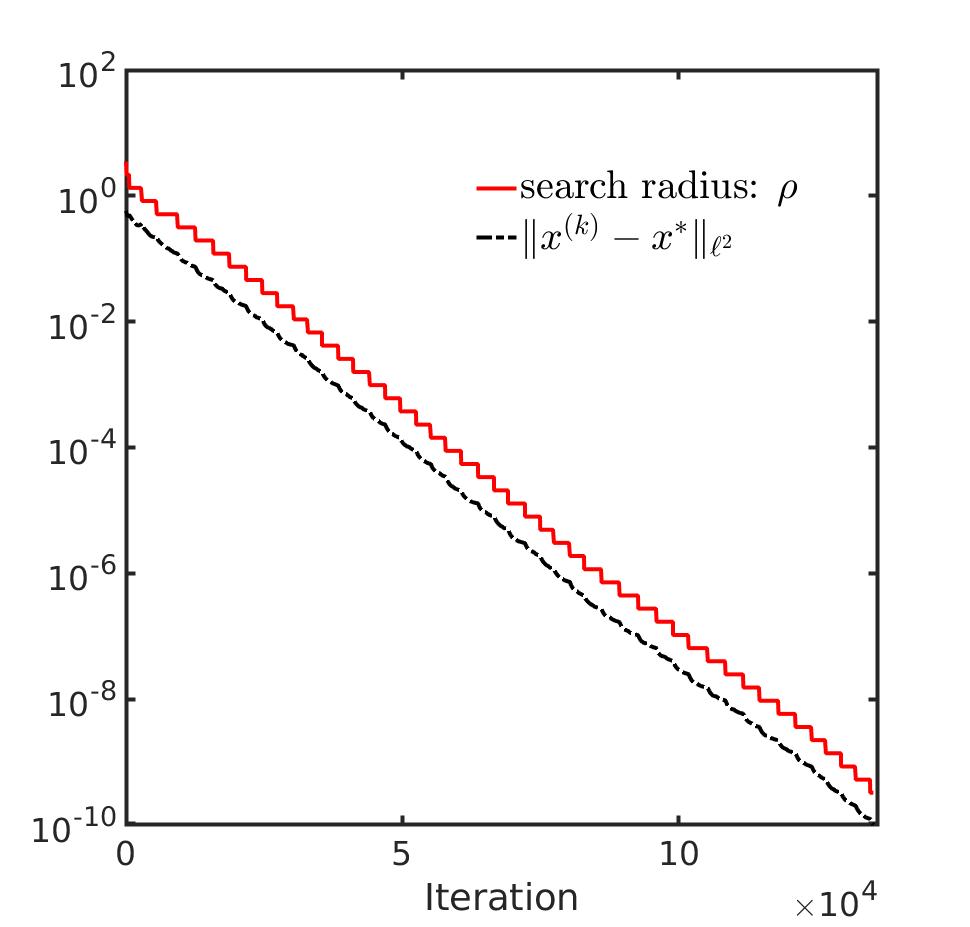
\includegraphics[scale=0.25]{../figures/ackley2500D_dist.png}
	  \caption{The iteration process of the adaptive HiCS method to 2500
	  dimensional Ackley function with initial search
	  radius $\rho_0=3.5$. Start point is randomly generated in the
	  space $[-10, 10]^{2500}$. } 
	\label{fig:ackley2500D:AHiCS}
\end{figure}

%\subsection{Other benchmark functions}
%
%Here we consider some benchmark functions in unconstrained
%optimization, including the Woods, Arwhead, Chrosen
%functions\,\cite{lukvsan2010modified, powell2006newuoa,
%andrei2008unconstrained}.

%\subsubsection{Powell function}
%\label{subsec:powell}
%
%\begin{align}
%    f(x) = \sum_{i=1}^{n/4}[(x_{4i-3}+10 x_{4i-2})^2 +
%    5(x_{4i-1}-x_{4i})^2 + (x_{4i-2}-2 x_{4i-1})^4 +
%    10(x_{4i-3}-x_{4i})^4]
%    \label{}
%\end{align}
%The function is usually evaluated on the hypercube $x_i\in[-4,5]$
%for all $i=1,\dots,n$.
%
%\textbf{available}


%\subsubsection{\textcolor{red}{Woods function}}
%\label{subsec:woods}
%
%The Woods function is a large and difficult problem in the CUTE test
%set\,\cite{lukvsan2010modified}. Its specified expression is  
%\begin{equation}
%    \begin{aligned}
%        f(x) = \sum^{n/4}_{i=1} \Big[100(x_{4i-2}-x^2_{4i-3})^2 +
%        (1-x_{4i-3})^2 + 90(x_{4i}-x_{4i-1})^2 +
%        \\
%        (1-x_{4i-1})^2 + 10(x_{4i-2}+x_{4i}-2)^2 +
%        0.1(x_{4i-2}-x_{4i})^2
%        \Big].
%    \end{aligned}
%    \label{eq:woods}
%\end{equation}
%The global minimizer is $x^*=(1,1,\dots,1)$ with $f(x^*)=0$.
%Here we choose the hard initial value\,\cite{lukvsan2010modified}, $x_j^{(0)}=-3.0$ if
%$j$ is even, and  $x_j^{(0)}=-1.0$ if $j$ odd, to test the
%HiCS method with $n=320$ and $\rho=5.0$. 
%The HiCS approach spends $111$ iterations to find a SMP. Then we
%can successively decrease the search radius by setting the
%control factor $\eta=0.5$.
%Tab.\,\ref{tab:woods320D} gives the iteration information when
%changing $\rho$ four times, including the number of iterations,
%the $\ell^2$-distance between convergent iterate and the global
%minimizer, and the convergent function value for each $\rho$.
%It can be found that the HiCS method can converge for each fixed
%search radius.
%\begin{table}[!htbp]
%\caption{Iteration information of applying the HiCS method to
%$320$ dimensional Woods function through successively decreasing
%$\rho$.}
%\label{tab:woods320D}
%\begin{center}
%\begin{tabular}{|c|c|c|c|}
% \hline
%  $\rho$ &  Iter. & $\ell^2$-distance & $f(x)$
% \\\hline
%5.0 &  \makecell{ 111 } & 2.0269797302e+01 & 1.9462281448e+04 
% \\\hline
%2.5 &  \makecell{ 21 } & 2.1446697698e+01 & 1.7213410433e+04
% \\\hline
%1.25&  \makecell{ 38 } & 2.3007762412e+01 & 1.4027762445e+04
% \\\hline
%0.625& \makecell{ 49 } & 2.1442322133e+01 & 9.2058823364e+03
%% \\\hline
%%0.3125&  \makecell{ 558 } & 1.8950544937e+01 & 2.3646230729e+03
%% \\\hline
%%0.15625&  \makecell{ 634 } & 1.6684359010e+01 & 1.2099516621e+03
%% \\\hline
%%0.078125&  \makecell{ 2502 } & 1.2212940331e+01 & 2.9382990538e+02
%% \\\hline
%% $\downarrow$ & $\downarrow$ & $\downarrow$  & $\downarrow$
%% \\\hline
%%1.907349e-05 & 114180  & 4.4027298178e-02 & 7.0921802110e-04 
%\\ \hline
%\end{tabular}
%\\
%%It costs $48665367$ function evaluations.
%\end{center}
%\end{table}
%Certainly, we can continue to apply the adaptive HiCS approach with
%$\eta=0.5$ to approximate the minimizer of Woods functions based
%on the above convergent results. The convergent procedure can be
%found in Fig.\,\ref{fig:woods}.
%\begin{figure}[!htbp]
%    \centering
%      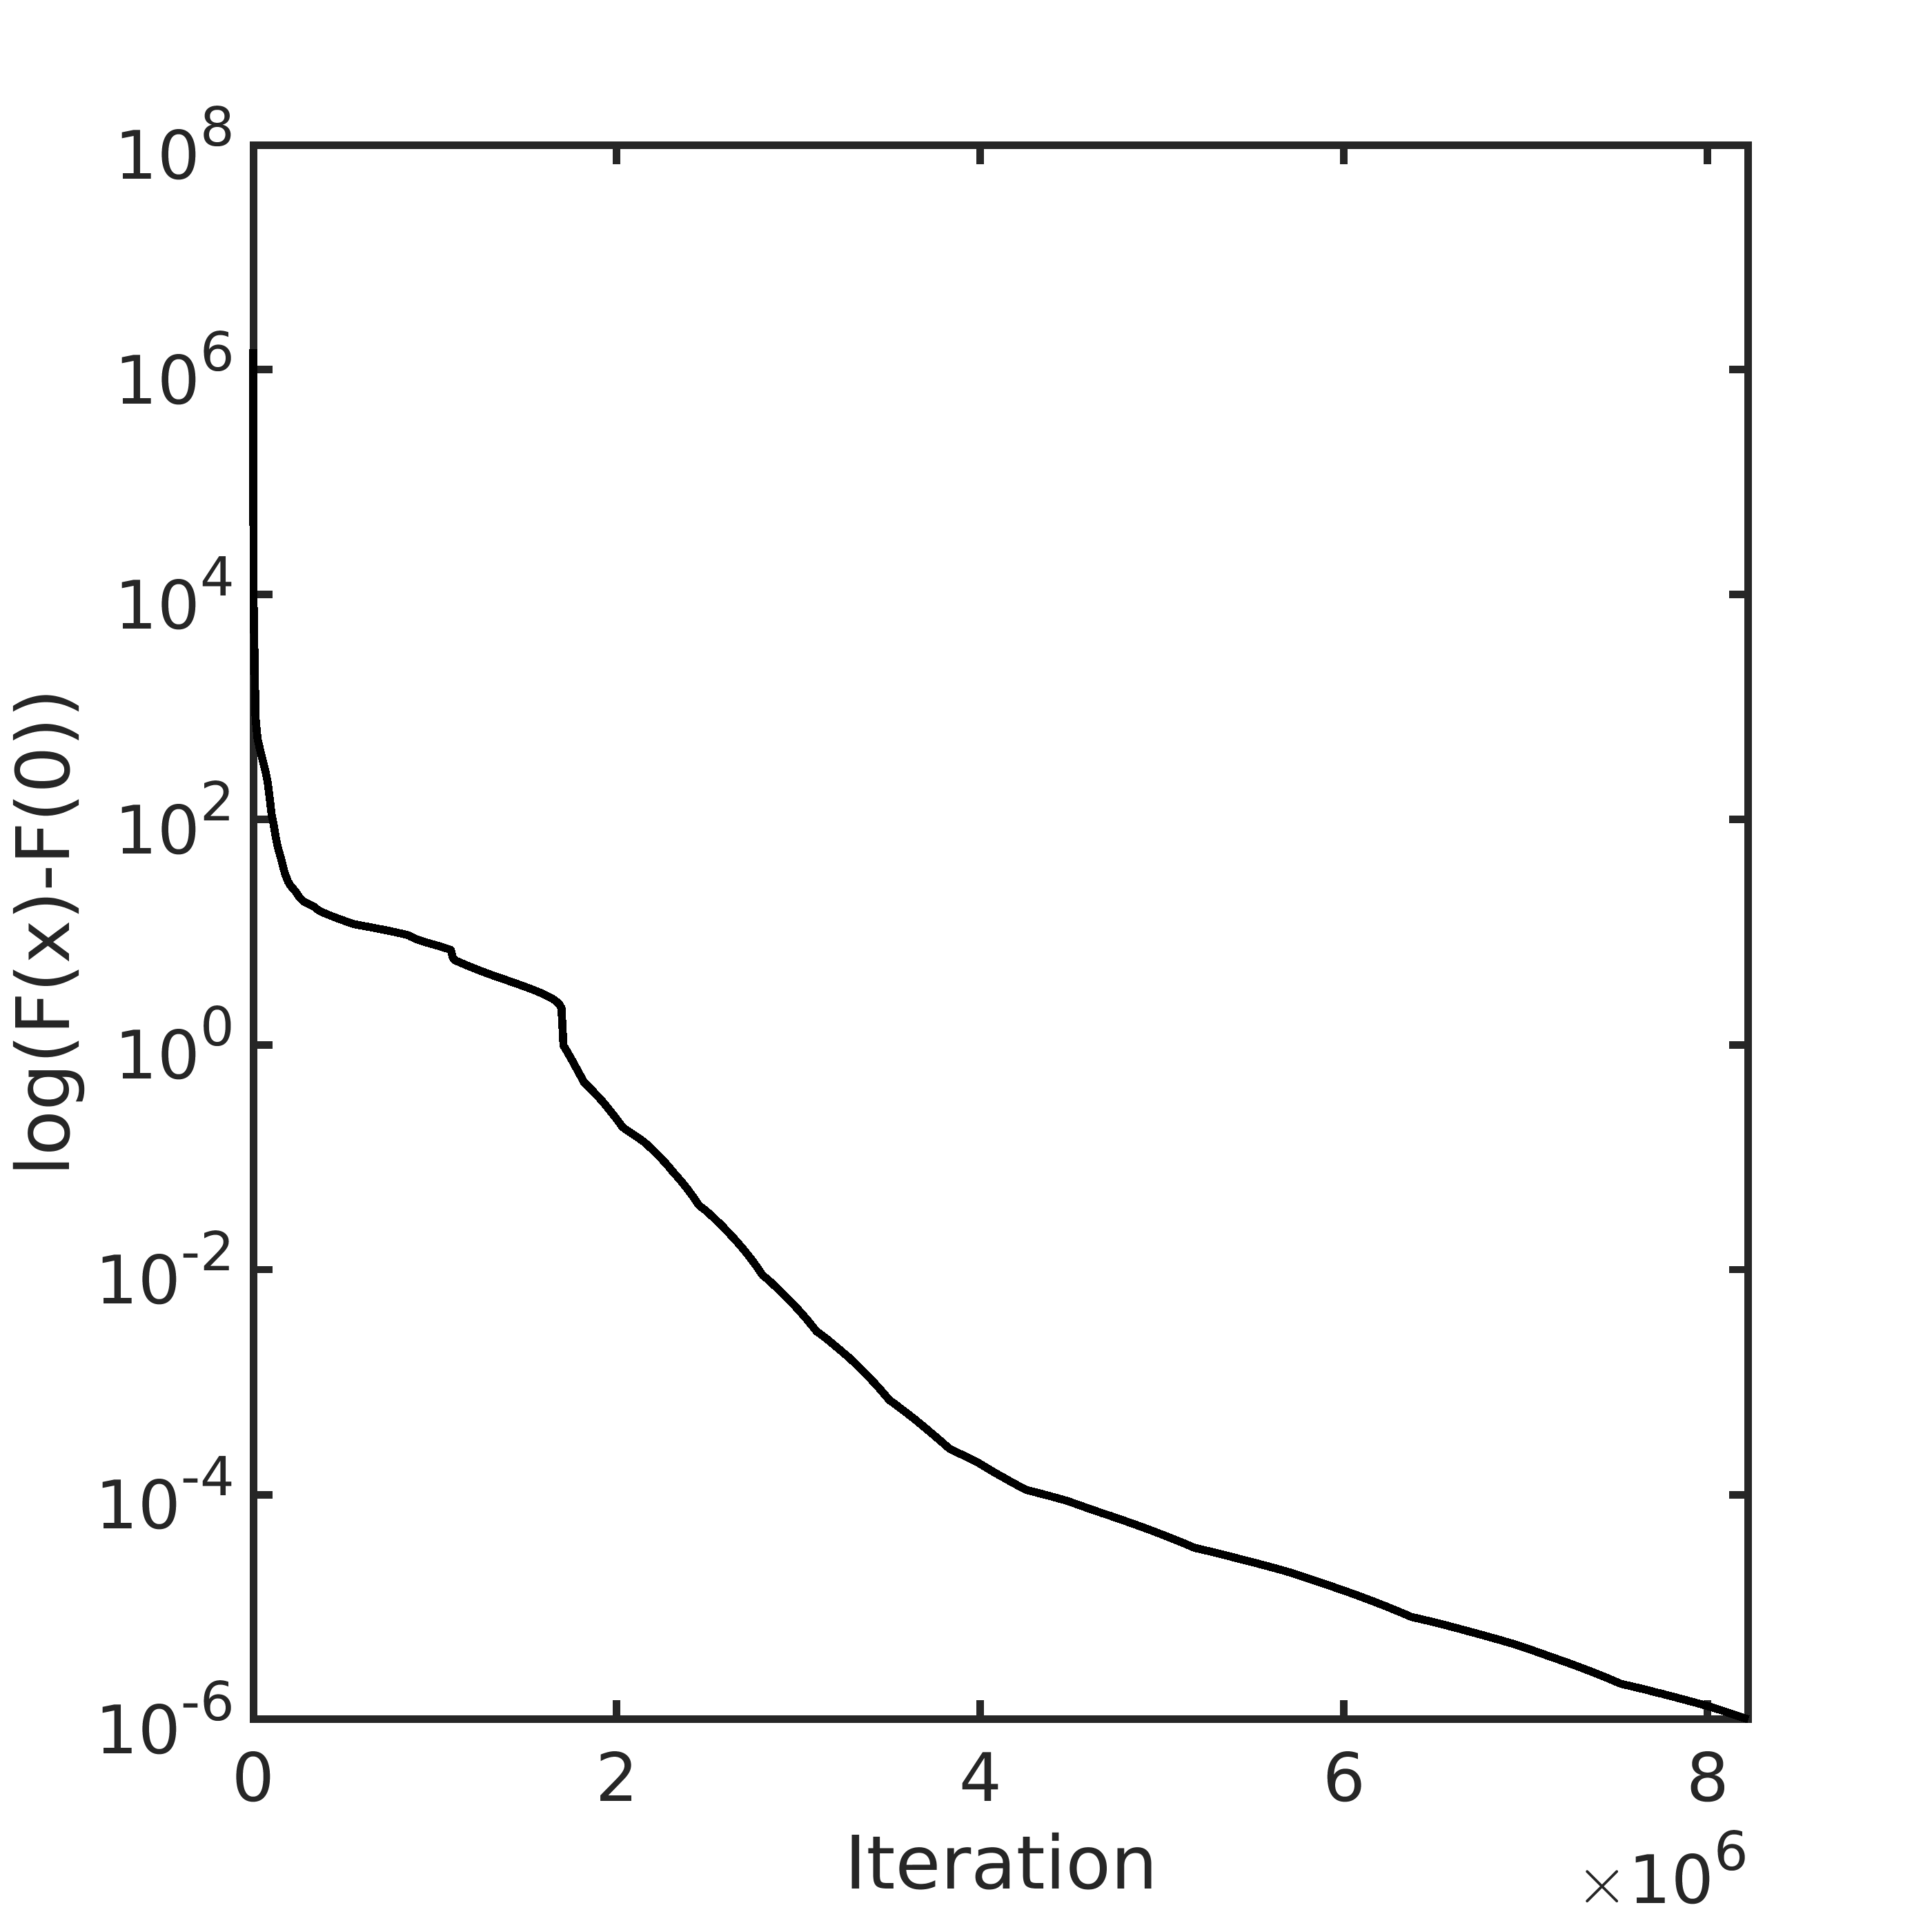
\includegraphics[scale=0.15]{../figures/woods320D.png}
%      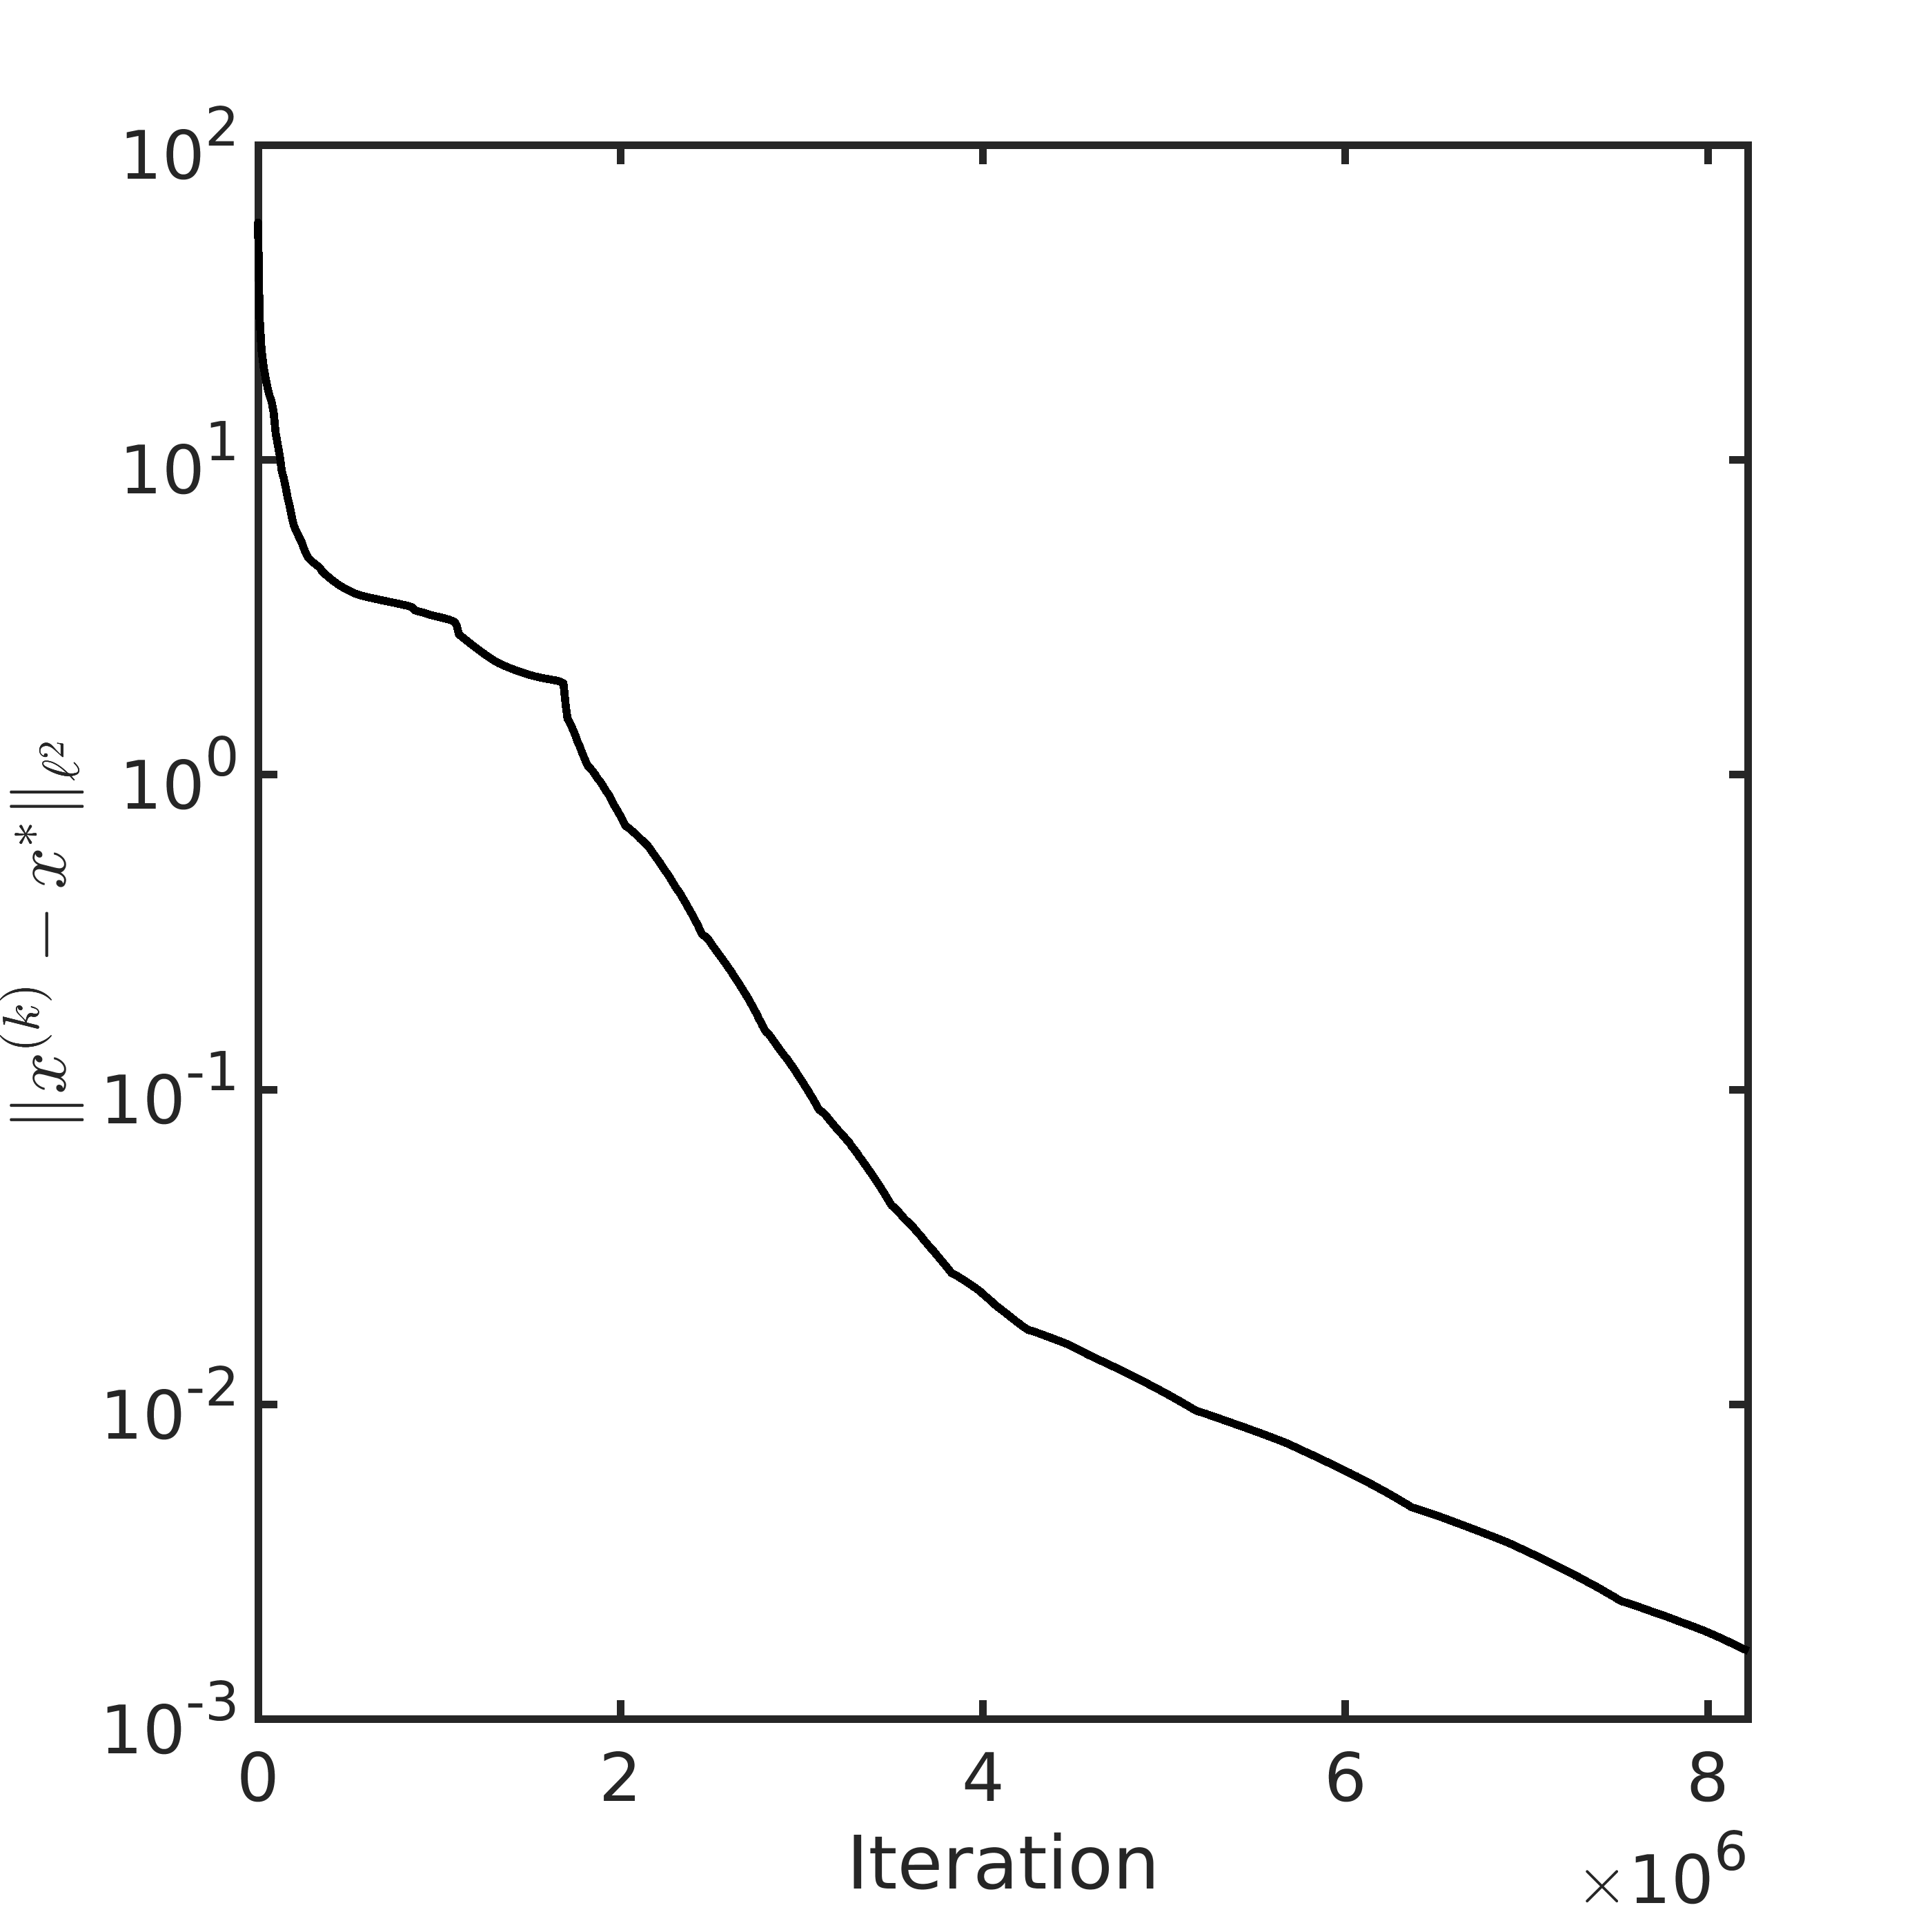
\includegraphics[scale=0.15]{../figures/woods320D_dist.png}
%  \caption{The iteration process of the adaptive HiCS method
%  ($\eta=0.5$) to the $320$ dimensional Woods function.}
%    \label{fig:woods}
%\end{figure}
%It is easy to find that the adaptive HiCS can further approximate the
%global minimizer as the iterations increase and the search radius
%decreases.
%
%\subsection{Arwhead function}
%\label{subsec:arwhead}
The last benchmark example is the Arwhead function, which has been
also used by Powell to test the NEWUOA derivative-free
method\,\cite{powell2006newuoa}. The expression of the Arwhead function is
\begin{align}
	f(x) = \sum_{i=1}^{d-1}[(x_i^2+x_n^2)^2 - 4 x_i +3].
	\label{}
\end{align}
The least value of $f$ is zero, which occurs when the minimizer
$x^*$ take the values $x_j=1$, $j=1,2,\dots,d-1$ and $x_d=0$. 
We directly apply the adaptive HiCS method ($\eta=0.5$) to $1000$
dimensional Arwhead function.
The starting vector is given by $x_j^{(0)}=1$, $j=1,2,\dots,d$, as
Powell done in Ref.\,\cite{powell2006newuoa}
The initial search radius $\rho_0=3$ and $\eta=(\sqrt{5}-1)/2$.
\begin{figure}[!htbp]
	\centering
	  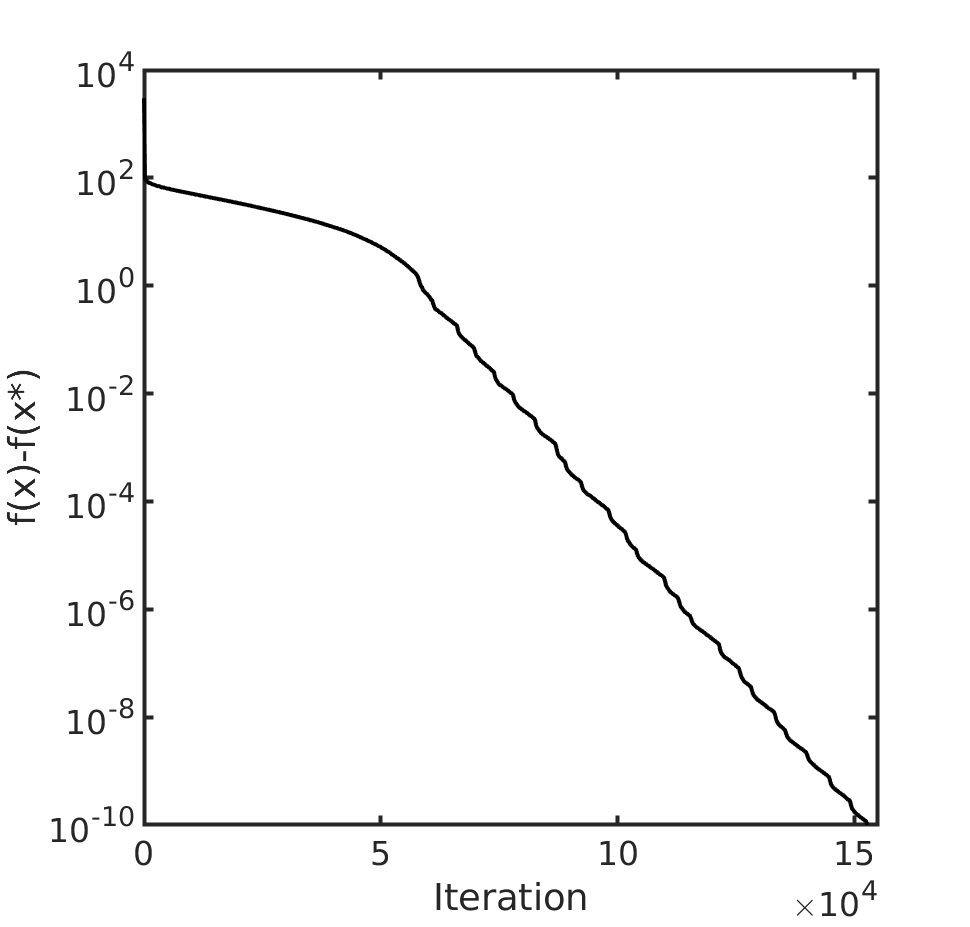
\includegraphics[scale=0.25]{../figures/arwhead1000D.png}
	  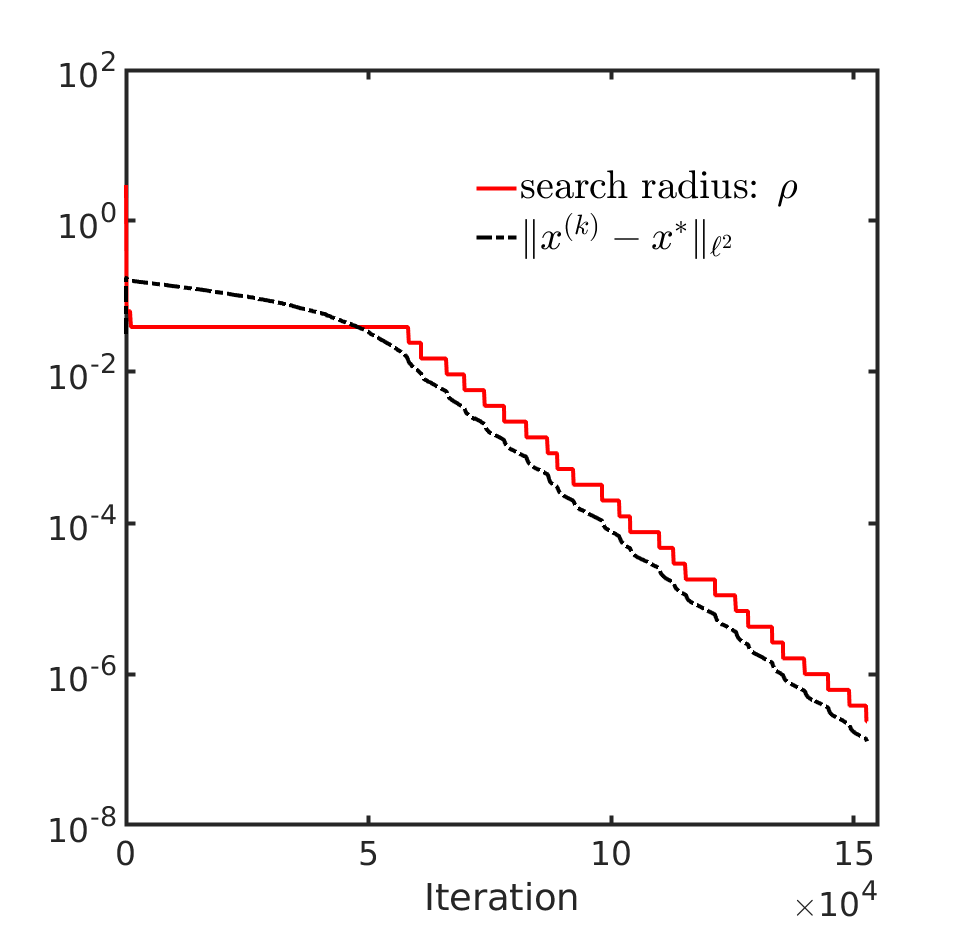
\includegraphics[scale=0.25]{../figures/arwhead1000D_dist.png}
  \caption{The iteration process of the adaptive HiCS method
  ($\eta=(\sqrt{5}-1)/2$) to the $1000$ dimensional Arwhead function.}
	\label{fig:arwhead}
\end{figure}

Fig.\,\ref{fig:arwhead} gives the iteration process of
applying the adaptive HiCS algorithm to $1000$ dimensional Arwhead function.
Obviously, the sequences of function values and iterators both
approximate the global minimum and the global minimizer, respectively. 
The function value always decreases as the proposed algorithm
indicates. While the distance $\|x^{(k)}-x^*\|_{\ell^2}$
demonstrates more interesting phenomena. At the beginning, the
search radius $\rho$ is larger than the distance which means the global
minimizer $x^*$ is in the search neighbourhood. Then when the distance is
about $1.67\times 10^{-1}$, the $\rho$ is smaller than the
distance which indicates $x^*$ is not in the search neighbourhood. 
It means that the iterator locates in the valley of a local minimizer. 
However, as iteration evolves, the HiCS algorithm can jump out of
the trap of the local energy well, and again contains the global
minimizer in the search region.



%\subsubsection{Chrosen function}
%\label{subsec:chrosen}
%
%The expression of Chrosen function is 
%\begin{align}
%    f(x) = \sum_{i=1}^{n-1}[(4(x_i-x_{i+1}^2)^2 + (1-x_{i+1})^2].
%    \label{} \end{align}
%Its least value of $f$ is zero, which occurs when the variables take the values
%$x_j=1$, $j=1,2,\dots,n$.
%We consider the $100$ dimensional Chrosen function with start
%point $x_j^{0}=-1$, $j=1,2,\dots,n$, as Powell done\,\cite{powell2006newuoa}.
%We also apply the adaptive HiCS method to this problem with
%initial search radius $\rho_0=5$, and $\eta=0.5$.
%The iteration process is presented in Fig.\,\ref{fig:chrosen}.
%\begin{figure}[!htbp]
%    \centering
%      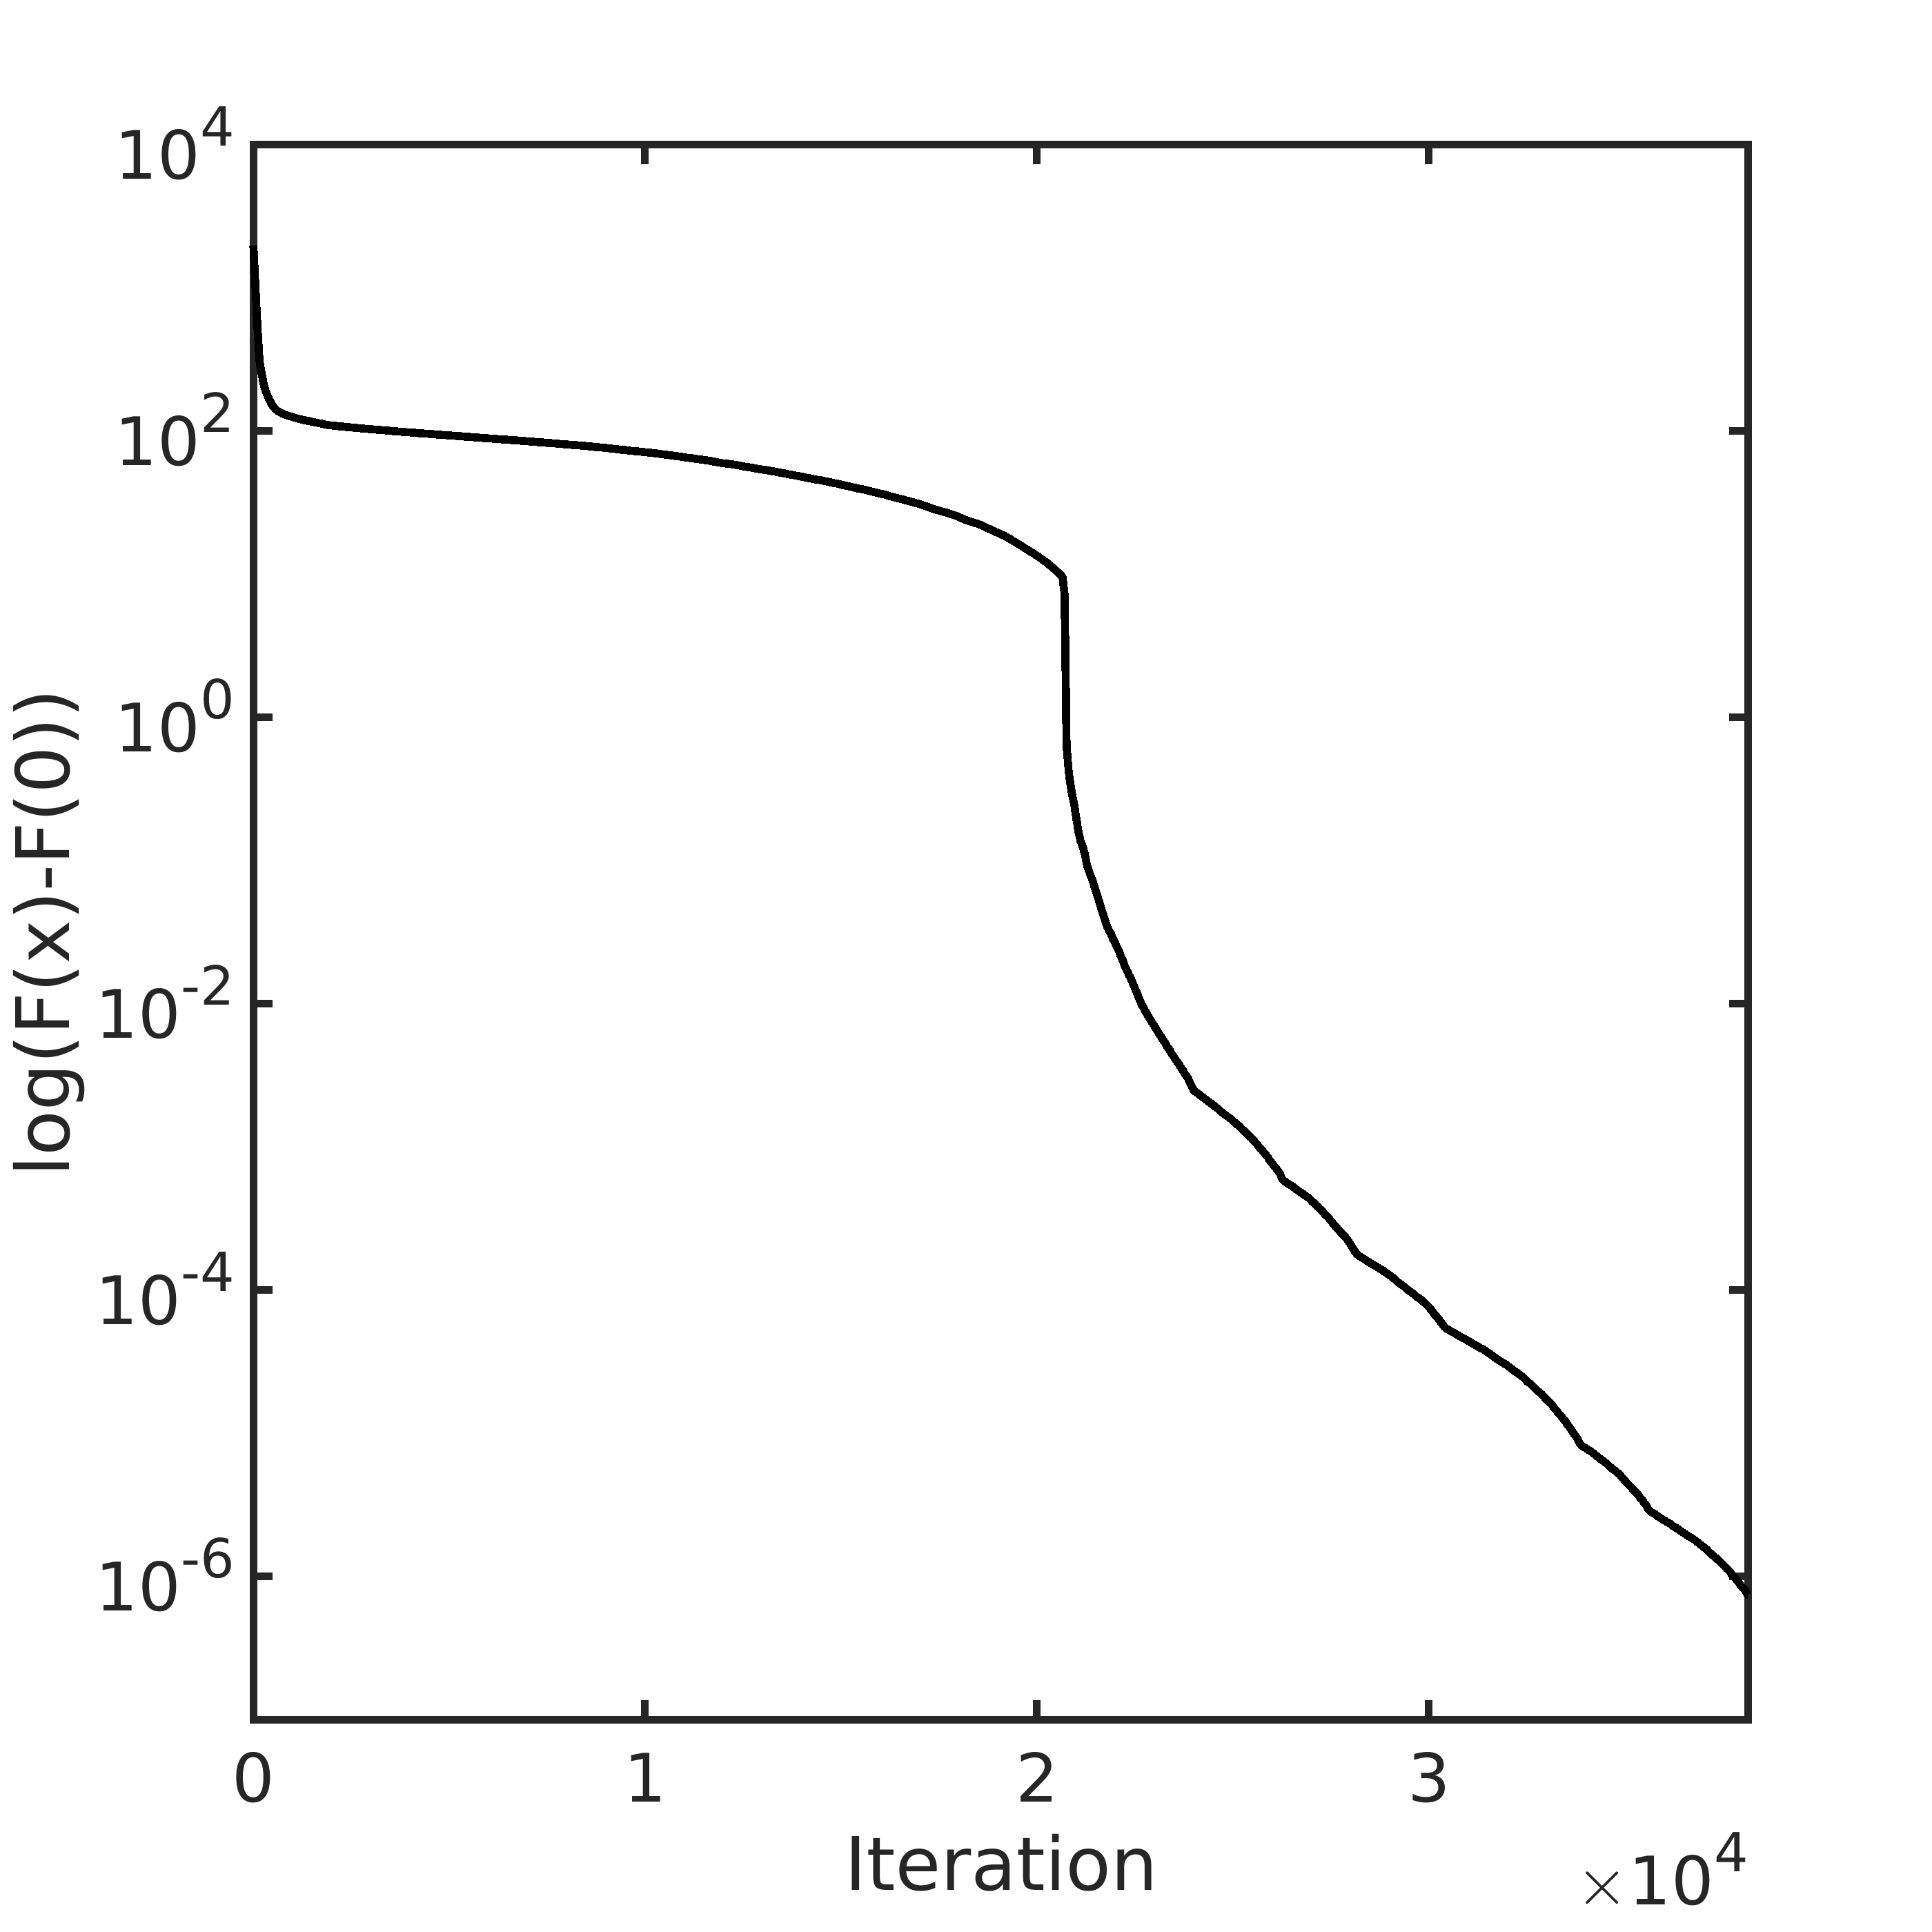
\includegraphics[scale=0.18]{../figures/chrosen100D.png}
%      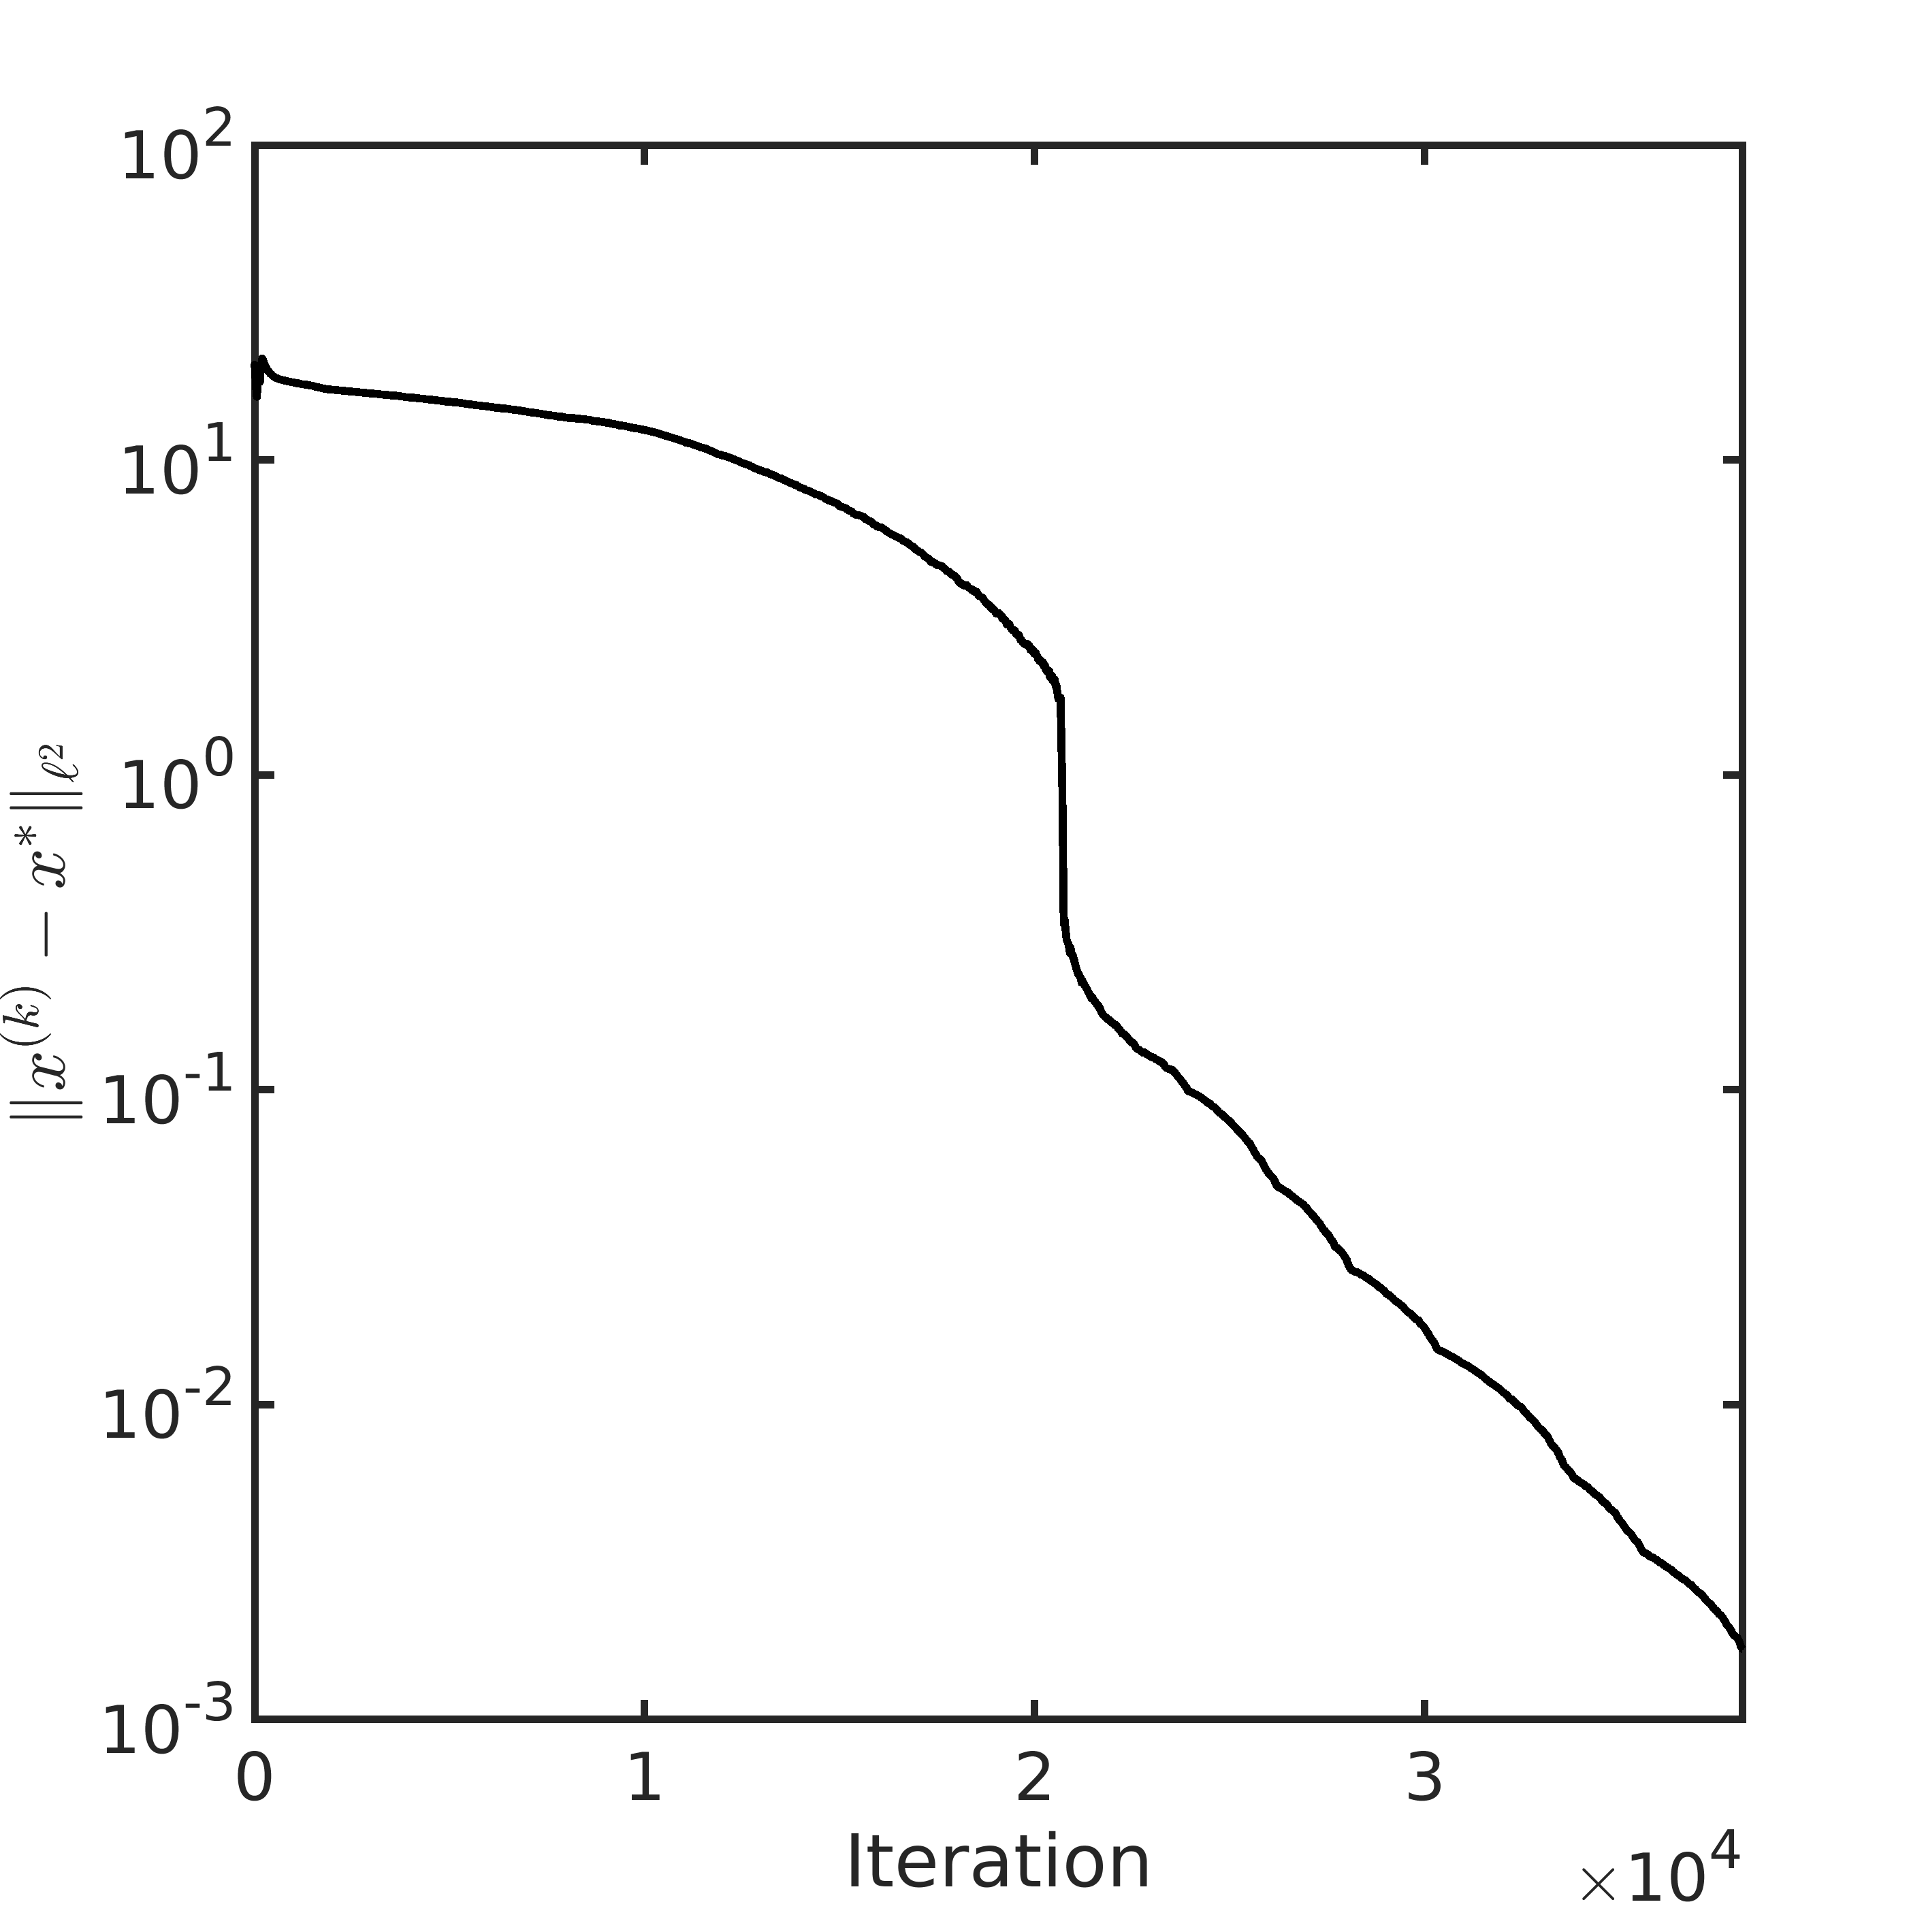
\includegraphics[scale=0.18]{../figures/chrosen100D_dist.png}
%  \caption{The iteration process of the adaptive HiCS method
%  ($\eta=0.5$) to the $100$ dimensional Chrosen function.}
%    \label{fig:chrosen}
%\end{figure}
%
%From Fig.\,\ref{fig:arwhead} and Fig.\,\ref{fig:chrosen}, one can
%find that the iteration processes are different for both 
%Arwhead and Chrosen functions which is attributed to the
%properties of objective functions. However, 
%the adaptive HiCS method is able to efficiently approximate the global
%minimizer for both functions. 
%
%It is hard to
%approach the minimizer by AHiCS algorithm. However, AHiCS method
%can approximate the minimizer using random initial value.



\section{Conclusion}
\label{sec:conclusion}

Inspired by the hill-climbing behavior of the blind, we have
proposed a new derivative-free method to unconstrained
optimization problems in our previous work\,\cite{huang2017hill}. 
In this paper, we establish a rigorous mathematical theory of the HiCS
algorithm which theoretically guarantees the finite-step convergence
under mild conditions. Numerical results also have demonstrated
the satisfactory property. 
In practice, the computational complexity of the HiCS algorithm mainly
depends on the discretized strategy on search boundary.
%In our previous work, the number of discretized points
%increases exponentially with the dimension of problems. It restricts
%the application to the high-dimensional optimization. 
To deal with high-dimensional problems, in this work, 
we proposed a new strategy of simplex
discretization method to save computational amount. Using the
simplex method, the number of function valuations is linearly
dependent on the dimension of problems,
which allows us to solve high dimensional optimization problems. 
Finally we demonstrate the efficiency of our proposed algorithm
through solving several higher dimensional benchmark problems.




\begin{thebibliography}{99}

\bibitem{sun2006optimization}
W.~Y.~Sun and Y.~Yuan,
Optimization theory and methods: nonlinear programming,
New York: Springer, 2006.

%\bibitem{conn2000trust}
%A.~R.~Conn, N.~I.~M.~Gould and P.~L.~Toint,
%Trust region methods, Philadelphia: SIAM, 2000.

\bibitem{nocedal2006numerical}
J.~Nocedal and S.~J.~Wright,
Numerical optimization, 
Berlin: Springer-Verlag, 2nd ed., 2006.

\bibitem{conn2009introduction}
A.~R.~Conn, K.~Scheinberg and L.~N.~Vicente,
Introduction to derivative-free optimization,
Philadelphia: SIAM, 2009.

\bibitem{huang2017hill}
{Y.~Huang and K.~Jiang,}
{Hill-Climbing Algorithm with a Stick for Unconstrained Optimization Problems},
{Adv. Appl. Math. Mech.},
2017, 9: 307--323.

\bibitem{dieterich2012empirical}
J.~M.~Dieterich and B.~Hartke, 
Empirical review of standard benchmark functions using evolutionary global optimization,
{Appl. Math.} 2012, 3: 1552--1564.

\bibitem{back1996evolutionary}
T.~B{\"a}ck, 
Evolutionary algorithms in theory and practice: evolution
  strategies, evolutionary programming, genetic algorithms,
Oxford University Press, 1996.

\bibitem{powell2006newuoa}
M.~J.~D.~Powell,
The NEWUOA software for unconstrained optimization without derivative, in
Large-Scale Nonlinear Optimization , eds. G.~Di~Pillo
and M.~Roma, Springer (New York), 2006, 255~297.


%%\bibitem{rios2013derivative}
%%L.~M.~Rios and N.~V.~Sahinidis,
%%Derivative-free optimization: a review of algorithms and comparison
%%  of software implementations.
%%{J. Global Optim.}, 2013, 56: 1247--1293.
%%
%\bibitem{powell2000uobyqa}
%M.~J.~D.~Powell, UOBYQA: unconstrained optimization by quadratic
%approximation, Technical Report DAMTP NA2000/14, CMS, University
%of Cambridge, 2000.
%
%\bibitem{powell2002trust}
%M.~J.~D.~Powell, On trust region methods for unconstrained
%minimization without derivatives, Technical Report DAMTP
%NA2002/NA02, CMS, University of Cambridge, February 2002.
%
%%\bibitem{wu2009heuristic}
%%T.~Wu, Y.~Yang, L.~Sun, and H.~Shao, A heuristic
%%iterated-subspace minimization method with pattern search for
%%unconstrained optimization, 
%%Comput. Math. Appl., 2009, 58: 2051-2059.
%%
%\bibitem{zhang2014sobolev}
%Z.~Zhang, Sobolev seminorm of quadratic functions with
%applications to derivative-free optimization, Math. Program.,
%2014, 146: 77-96.
%
%\bibitem{michalewicz2004how}
%Z. Michalewicz and D. B. Fogel, How to solve it: modern
%heuristics, Springer, 2004.
%
%%\bibitem{lecun2015deep}
%%Y.~LeCun, Bengio, Y.~Hinton, G.~Hinton, Deep learning, Nature,
%%2015, 521: 521-436.
%%
%%\bibitem{hooke1961direct}
%%R.~Hooke and T.~A.~Jeeves,
%%``Direct search'' solution of numerical and statistical problems,
%%{J. ACM}, 1961, 8: 212--229.
%%
%\bibitem{lewis2000direct}
%R.~M.~Lewis, V.~Torczon and M.~W.~Trosset,
%Direct search methods: then and now,
%{J. Comput. Appl. Math.},
%2000, 124: 191--207.
%
%\bibitem{nelder1965simplex}
%J.~A.~Nelder and R.~Mead,
%A simplex method for function minimization,
%{Comput. J.}, 1965, 7: 308--313.
%
%\bibitem{torczon1997convergence}
%V.~Torczon,
%On the convergence of pattern search algorithms,
%{SIAM J. Optim.}, 1997, 7: 1--25.
%
%\bibitem{kolda2003optimization}
%T.~G.~Kolda, R.~W.~Lewis and V.~Torczon,
%Optimization by direct search: new perspectives on some classical
%and modern methods,
%{SIAM Rev.}, 2003, 45: 385--482.
%
%\bibitem{dennis1991direct}
%J.~E.~Jr Dennis and V.~Torczon,
%Direct search methods on parallel machines,
%{SIAM J. Optim.}, 1991, 1: 448--474.
%
%\bibitem{gratton2015direct} 
%S.~Gratton, C.~W.~Royer, L.~N.~Vicente, Z.~Zhang, Direct search
%based on probabilistic descent, SIAM J.~Optim., 
%2015, 25:1515-1541.
%
%\bibitem{russell2010artificial} 
%S.~J.~Russell and P.~Norvig,  Artificial intelligence: a modern
%approach, 3rd ed., Prentice Hall, 2010.
%
%\bibitem{dennis1987optimization}
%J.~E.~Jr Dennis and D.~J.~Woods,
%Optimization on microcomputers: The Nelder-Mead simplex algorithm.
%In: New computing environments: microcomputers in large-scale
%computing, A.~Wouk ed., Philadelphia: SIAM, 1987.
%
%%\bibitem{lukvsan2010modified}
%%L.~Luk{\v{s}}an, C.~Matonoha, J.~Vlcek,
%%Modified CUTE problems for sparse unconstrained optimization,
%%Techical Report,
%%2010, 1081.
%
%%\bibitem{algopy}
%%https://pythonhosted.org/algopy/index.html
%
%%\bibitem{andrei2008unconstrained}
%%N.~Andrei, 
%%An unconstrained optimization test functions collection,
%%Adv. Model. Optim.,
%%2008, 10: 147--161.


\end{thebibliography}


\end{document}
